%%%%%%%%%%%%%%%%%%%%%%%%%%%%%%%%%%%%%%%%%
% kaobook
% LaTeX Template
% Version 1.3 (December 9, 2021)
%
% This template originates from:
% https://www.LaTeXTemplates.com
%
% For the latest template development version and to make contributions:
% https://github.com/fmarotta/kaobook
%
% Authors:
% Federico Marotta (federicomarotta@mail.com)
% Based on the doctoral thesis of Ken Arroyo Ohori (https://3d.bk.tudelft.nl/ken/en)
% and on the Tufte-LaTeX class.
% Modified for LaTeX Templates by Vel (vel@latextemplates.com)
%
% License:
% CC0 1.0 Universal (see included MANIFEST.md file)
%
%%%%%%%%%%%%%%%%%%%%%%%%%%%%%%%%%%%%%%%%%

%----------------------------------------------------------------------------------------
%	PACKAGES AND OTHER DOCUMENT CONFIGURATIONS
%----------------------------------------------------------------------------------------

\documentclass[
	a4paper, % Page size
	fontsize=12pt, % Base font size
	twoside=false, % Use different layouts for even and odd pages (in particular, if twoside=true, the margin column will be always on the outside)
	%open=any, % If twoside=true, uncomment this to force new chapters to start on any page, not only on right (odd) pages
	%chapterentrydots=true, % Uncomment to output dots from the chapter name to the page number in the table of contents
	numbers=noenddot, % Comment to output dots after chapter numbers; the most common values for this option are: enddot, noenddot and auto (see the KOMAScript documentation for an in-depth explanation)
]{kaobook}


\newcommand{\optmargintoc}[0]{%
    \margintoc%
}

\newcommand\abstractname{Abstract}  %%% here
\makeatletter
\if@titlepage
  \newenvironment{abstract}{%
      \titlepage
      \null\vfil
      \@beginparpenalty\@lowpenalty
      \begin{center}%
        \bfseries \abstractname
        \@endparpenalty\@M
      \end{center}}%
     {\par\vfil\null\endtitlepage}
\else
  \newenvironment{abstract}{%
      \if@twocolumn
        \section*{\abstractname}%
      \else
        \begin{center}%
          {\bfseries \abstractname\vspace{-.5em}\vspace{\z@}}%
        \end{center}%
        \quotation
      \fi}
      {\if@twocolumn\else\endquotation\fi}
\fi
\makeatother

\newcommand{\subcappar}{%
    \Centering% center text
    \setlength{\RaggedRightParindent}{0em}% Suppress indentation
    \setlength{\parindent}{0em}% Suppress indentation
    \setlength{\parskip}{0.5pc}% Set the space between paragraphs
    %%\singlespacing% Set the space between lines
    \frenchspacing% No additional space after periods
    \normalfont% Use the default font
    \footnotesize% Use a smaller size
}
\DeclareCaptionFormat{subcap}{\subcappar #1#2#3}

% \newcommand{\boxedsidenote}[2][]{\sidenote{\begin{kaobox}[title=#1]{#2}\end{kaobox}}}

\newcommand{\adummy}{}%

% This should sort out centring for short figure/* captions
\captionsetup[figure]{format=plain,singlelinecheck=true}

% Choose the language
\ifxetexorluatex
	\usepackage{polyglossia}
	\setmainlanguage{english}
\else
	\usepackage[english]{babel} % Load characters and hyphenation
\fi
\usepackage[english=british]{csquotes}	% English quotes

% Load packages for testing
\usepackage{blindtext}
%\usepackage{showframe} % Uncomment to show boxes around the text area, margin, header and footer
%\usepackage{showlabels} % Uncomment to output the content of \label commands to the document where they are used

% Load the bibliography package
\usepackage[maxbibnames=6,backref=false]{kaobiblio}
\addbibresource{main.bib} % Bibliography file

% Load mathematical packages for theorems and related environments
\usepackage[framed=true]{kaotheorems}

% Load the package for hyperreferences
\usepackage{kaorefs}

\usepackage{amsmath}
\usepackage{amstext}
\usepackage{gensymb}
\usepackage{units}
\usepackage[utf8]{inputenc}
\usepackage{setspace}
\usepackage{float}
\usepackage{pdfpages}
\usepackage{fullwidth}
\usepackage{caption}
\usepackage{subcaption}
\usepackage{graphicx}
\usepackage{bbold}
\usepackage{truncate}

\renewcommand{\baselinestretch}{1.25} 

\setcounter{margintocdepth}{\sectiontocdepth}
\addtocontents{toc}{\protect\setcounter{tocdepth}{\sectiontocdepth}}

\makeindex[columns=3, title=Alphabetical Index, intoc] % Make LaTeX produce the files required to compile the index

\newcommand{\etalcite}[1]{%
    \citeauthor*{#1}~\sidecite{#1}%
}

\makeatletter
\def\invisiblesection#1{%
\refstepcounter{section}%
  \addcontentsline{toc}{section}{\protect\numberline{\thesection}#1}%
  \mtocsection{#1}
%   \margin
  \sectionmark{#1}\phantom{}
  \protected@edef\@currentlabelname{#1} % Set correct name
}
\makeatother

\DeclareMathAlphabet{\mathcal}{OMS}{cmsy}{m}{n}

% \makeglossaries % Make LaTeX produce the files required to compile the glossary
% \newglossaryentry{computer}{
	name=computer,
	description={is a programmable machine that receives input, stores and manipulates data, and provides output in a useful format}
}

% Glossary entries (used in text with e.g. \acrfull{fpsLabel} or \acrshort{fpsLabel})
\newacronym[longplural={Frames per Second}]{fpsLabel}{FPS}{Frame per Second}
\newacronym[longplural={Tables of Contents}]{tocLabel}{TOC}{Table of Contents}

 % Include the glossary definitions

% \makenomenclature % Make LaTeX produce the files required to compile the nomenclature

% Reset sidenote counter at chapters
%\counterwithin*{sidenote}{chapter}

%----------------------------------------------------------------------------------------

\begin{document}

%----------------------------------------------------------------------------------------
%	BOOK INFORMATION
%----------------------------------------------------------------------------------------

% \titlehead{The \texttt{kaobook} class}
\subject{Doctoral Thesis}

\title{Hydrodynamics of Ciliary Systems}
\subtitle{
    Department of Living Matter Physics \\
    Max Planck Institute for Dynamics and Self-Organisation
}

\author{David Hickey}

\date{December 2022}

% \publishers{An Awesome Publisher}

%----------------------------------------------------------------------------------------

\frontmatter % Denotes the start of the pre-document content, uses roman numerals

\makeatother


%----------------------------------------------------------------------------------------
%	OUTPUT TITLE PAGE AND PREVIOUS
%----------------------------------------------------------------------------------------

% Note that \maketitle outputs the pages before here

% \maketitle

\begin{centering}

    \vspace*{1cm}

	\noindent {\Huge Hydrodynamics of Ciliary Systems}
	\vspace*{2.0cm}
	
	\noindent {\large Dissertation for the award of the degree}\vspace*{0.5cm}
	
	\noindent {\LARGE \textsc{Doctor Rerum Naturalium}}\vspace*{0.5cm}
	
	\noindent {\large of the Georg-August-Universität Göttingen}\vspace*{1.2cm}
	
	
	
	
	\noindent {\large within the doctoral program}\vspace*{0.5cm}
	
	\noindent {\LARGE \textsc{Physics of Biological and Complex Systems}}\vspace*{0.5cm}
	
	\noindent {\large of the Georg-August University School of Science}\vspace*{1.2cm}
	
	
	
	\noindent {\large submitted by}\vspace*{0.5cm}
	
	\noindent {\LARGE \textsc{David James Hickey}}\vspace*{0.5cm}
	
	\noindent {\large from}\vspace*{0.5cm}
	
	\noindent {\LARGE \textsc{Epsom, The United Kingdom}}\vspace*{3.0cm}
	
	{\Large 
\includegraphics[width=0.3\textwidth]{images_other/uni-goe-logo.png} \hfill Göttingen \the\year{}}
	
	
\end{centering}

\clearpage

\subsection*{Thesis committee}
{
	\begin{tabular}{rl}
		Member 1 & Prof. Dr. Ramin Golestanian \\
		& Living Matter Physics \\
		& Max-Planck-Institut für Dynamik und Selbstorganisation \vspace*{0.25cm} \\
		Member 2 & Prof. Dr. Marcus Müller \\
		& Institut für Theoretische Physik \\ & Georg-August-Universität Göttingen \vspace*{0.25cm} \\
		Member 3 & Prof. Dr. Annette Zippelius \\
		& Institut für Theoretische Physik \\ & Georg-August-Universität Göttingen \vspace*{-0.0cm} \\
		\hspace*{\widthof{Additional Reviewer}} &
	\end{tabular}
}
\vspace*{-0.25cm}
\subsection*{Members of the examination board}
{
	\begin{tabular}{rl}
		First referee & Prof. Dr. Ramin Golestanian \\
		& Living Matter Physics \\
		& Max-Planck-Institut für Dynamik und Selbstorganisation \vspace*{0.25cm} \\
		Second referee & Prof. Dr. Marcus Müller \\
		& Institut für Theoretische Physik \\ & Georg-August-Universität Göttingen \vspace*{0.25cm} \\
		Additional reviewer & Prof. Dr. Annette Zippelius \\
		& Institut für Theoretische Physik \\ & Georg-August-Universität Göttingen \vspace*{0.25cm} \\
		Additional reviewer & Prof. Dr. Stefan Klumpp \\
		& Institute for Nonlinear Dynamics \\ & Georg-August-Universität Göttingen \vspace*{0.25cm} \\
		Additional reviewer & Dr. David Zwicker \\
		& Theory of Biological Fluids \\ & Max-Planck-Institut für Dynamik und Selbstorganisation \vspace*{0.25cm} \\
		Additional reviewer & Dr. Aljaz Godec \\
		& Mathematical Biophysics Group \\ & Max-Planck-Institut für Multidisziplinäre Naturwissenschaften \vspace*{1.2cm} \\
	\end{tabular}
}

Date of oral examination: 2023-06-29

\addcontentsline{toc}{chapter}{Abstract}
\begin{abstract}
    The interactions of cilia with one another and their environment are central to many important questions in biology. These hairlike organelles are found in motile and immotile (or `primary') variants, and have a variety of roles in sensing and fluid pumping. Primary cilia have long been known to act as chemosensors, but recent research has found that motile cilia also have this ability, and it is not known what benefit is conferred by combining all the complicated required molecular machinery. These chemosensitive motile cilia are often found in bundles, which is surprising, as one would expect each to deplete the local chemical concentration field, leading to a lower sensitivity per cilium. Motile cilia have long been known to synchronise with one another to produce metachronal waves, but the precise mechanism behind this synchronisation is still not well understood, except that hydrodynamics plays an important role.
    
    In this thesis, we aim to make some headway in answering these open questions, by developing models of the interactions of cilia and the surrounding fluid flow. First, using both analytical and computational methods, we determine the mass transfer to individual cilia (both primary and motile) as well as bundles of motile cilia. We show that the cilium geometry alone is sufficient to dramatically increase chemosensitivity over chemosensors on the cell surface, especially if the fluid near the cilium is in motion. We also find that motility can increase chemosensitivity by a large factor at realistic cilium speeds, and that motile bundles are more chemosensitive per cilium, provided they are beating sufficiently quickly. We then use computational methods to focus on how cilia hydrodynamically interact with one another, and show that certain cilium beats can result in strongly nonreciprocal hydrodynamic interactions that can give rise to quickly emerging metachronal order with a single dominant wavevector, even in finite systems. When the near-field hydrodynamic interactions (and hence the nonreciprocity of interactions) is suppressed, synchronisation is much slower and multiple wavevectors are seen.
    
    We have therefore uncovered several reasons why chemosensors may be advantageously located on both motile and primary cilia, and shown that a cilium beat fine-tuned to give strong nonreciprocal interactions can be extremely effective in inducing metachronal order. This amounts to a significant amount of evidence pointing to some potential answers to some of the open questions surrounding cilia.
\end{abstract}

\chapter*{Author contributions}
\addcontentsline{toc}{chapter}{Author contributions} % Add the preface to the table of contents as a chapter

This thesis contains two scientific articles, both included here in their original form.

Chapter~\ref{ch:results_particle} contains the article ``Ciliary chemosensitivity is enhanced by cilium geometry and motility'', published in the journal eLife, authored by David J Hickey, Andrej Vilfan, and Ramin Golestanian. The project on which the work was based was conceptualised by AV and RG; the analysis and simulation was designed and implemented by DJH and AV. The manuscript was written by DJH and AV, and edited by DJH, AV and RG. Supervision was contributed by AV and RG.

Chapter~\ref{ch:results_sync} contains the article ``Nonreciprocal interactions give rise to fast cilium synchronisation in finite systems'', currently under review in the journal PNAS, authored by David J Hickey, Ramin Golestanian, and Andrej Vilfan. The project on which the work was based was conceptualised by AV and RG; the analysis and simulation was designed and implemented by DJH and AV. The manuscript was written by DJH and AV, and edited by DJH, AV and RG. Supervision was contributed by AV and RG.

All other work and writing presented in the thesis is entirely the work of DJH. %\todo{come back if the PNAS paper changes state}

\clearpage

\chapter*{Acknowledgements}
\addcontentsline{toc}{chapter}{Acknowledgements} % Add the preface to the table of contents as a chapter

% This thesis summarises work conducted over a period of over three years, beginning in 2019 and ending now in 2023. The research presented here has been published in two different journals\todo{I bloody hope}, and has made its way to several conferences and summer schools in poster and presentation form.

This thesis summarises work conducted over a period of over three years, beginning in 2019 and ending now in 2023. Without the support I have received from others, this work could never have existed, so I would like to take this space to acknowledge their contributions:

I am grateful to my thesis advisory committee members, Prof. Dr. Marcus Müller and Prof. Dr. Annette Zippelius, as well as my supervisors, Prof. Dr. Ramin Golestanian and Dr. Andrej Vilfan, for their constant guidance and support. Of these, I would especially like to thank Andrej Vilfan -- I could not have asked for a better supervisor. These people have been the dynein arms that have been propelling me in the right direction.

I am grateful to everyone who proofread this thesis to make sure it was the best it could be, especially my parents, who have probably read through it more times than I have. Without them, this piece of writing would be like a kidney with no mechanosensitive cilia, i.e. missing some very important parts and being dramatically worse off as a result.

Lastly, if my time spent here has taught me anything, it is that collective behaviour is important at all scales of living systems: just as motile cilia are more efficient when they work in a group, life is much better when your friends have your back. For that reason, I'd like to thank everyone who I've enjoyed spending time with during the last three-and-a-bit years, in Göttingen and elsewhere. You know who you are!

\vspace{1cm}

Best wishes,

David

%----------------------------------------------------------------------------------------
%	PREFACE
%----------------------------------------------------------------------------------------
% \input{chapters/preface.tex}
% \index{preface}

%----------------------------------------------------------------------------------------
%	TABLE OF CONTENTS & LIST OF FIGURES/TABLES
%----------------------------------------------------------------------------------------

\begingroup % Local scope for the following commands

% Define the style for the TOC, LOF, and LOT
\setstretch{1} % Uncomment to modify line spacing in the ToC
%\hypersetup{linkcolor=blue} % Uncomment to set the colour of links in the ToC
\setlength{\textheight}{230\hscale} % Manually adjust the height of the ToC pages

% Turn on compatibility mode for the etoc package
\etocstandarddisplaystyle % "toc display" as if etoc was not loaded
\etocstandardlines % "toc lines" as if etoc was not loaded

\tableofcontents % Output the table of contents

% \listoffigures % Output the list of figures

% Comment both of the following lines to have the LOF and the LOT on different pages
% \let\cleardoublepage\bigskip
% \let\clearpage\bigskip
% 
% \listoftables % Output the list of tables

\endgroup

%----------------------------------------------------------------------------------------
%	MAIN BODY
%----------------------------------------------------------------------------------------

\mainmatter % Denotes the start of the main document content, resets page numbering and uses arabic numbers
\setchapterstyle{kao} % Choose the default chapter heading style

\setchapterpreamble[u]{\optmargintoc}
\chapter{Introduction}
\labch{intro}

% \begin{itemize}
%     \item Cool galaxy-brain hook (ca. 1 page, 300 words)
%     \item General stuff about active matter (ca. 1 page, 300 words)
%     \item Cilia are cool and everywhere and do really interesting stuff, and are awesome to research. (ca. 1 page, maybe a little over 300 words)
%     \item I think Mirna did this section \textit{really} well so let's just take a lot of inspiration from her layout.
% \end{itemize}

If one were to go through some of the anatomical sketches made by Leonardo da Vinci, one might find something unexpected: a drawing of someone with their heart on the right side of their chest, as opposed to the more usual left side. It's not certain whether he simply reflected the sketch as he famously reflected his handwriting, but this inversion is a real condition, known as \textit{situs inversus}\boxedsidenote[][-70pt]{If he really did observe \textit{situs inversus}, he didn't leave any record to indicate that he found it interesting or unusual. Partial inversions (usually called \textit{situs ambiguous}) were later explicitly described by Hieronymus Fabricius~\cite{pennekamp_situs_2015} and Marco Aurelio Severino~\cite{ogunlade_role_2015}, with the full inversion probably being first described later by Matthew Baillie~\cite{ogunlade_role_2015, baillie_xxi_1997}.}.\nosidecite[160pt]{pennekamp_situs_2015, ogunlade_role_2015, baillie_xxi_1997}
Approximately one in ten thousand people are born with this condition, where some or all the organs in the body are reflected left to right. Most patients have all their organs reflected and thus experience no major health issues, as the relative position of all organs is unchanged -- they might never even know of their unusual organ arrangement. 
% It's very possible to live an entire life with this condition without ever having the slightest inkling, finding out only during a medical scan or procedure that incidentally uncovers the unusual arrangement.
However, an unlucky few will experience only a partial reflection, leading to potentially life-altering complications~\sidecite[100pt]{eitler_situs_2022}. Even centuries on from the first descriptions, we still don't know exactly what causes this to happen. We do, however, know that tiny hairlike organelles named cilia play a central role~\sidecite[100pt]{essner_conserved_2002, mcgrath_cilia_2003}, just as they will play a central role in the work described in this thesis.

One can hardly blame the physician Matthew Baillie for describing this inversion as `remarkable' in a letter to a friend~\cite{baillie_xxi_1997}, but \textit{situs inversus} is far from the only fascinating or unexpected thing in biology. The billions of years that have been spent by natural selection tweaking and optimising living organisms have left us some incredibly complex and robust active systems that we are only just beginning to understand. Cilia and the associated disorders are just one very narrow example -- the wider field of active matter research concerns itself with systems from scales much smaller than cells (such as cilia or swimming microorganisms) to scales much greater than the size of organisms (such as flocking behaviour in sheep or crowd dynamics at sports venues). Nature has something of a head start on us, as the field of active matter research has existed for barely three decades -- possibly the best known model in active matter is the Vicsek model of flocking, which was only defined in 1995~\sidecite{vicsek_novel_1995}) -- whereas life on this planet may have existed for close to 4.5 billion years. However, there is a bright side to the rather daunting problem we find ourselves with, as we are presented with a unique opportunity to dig into these systems and begin to unravel the mysteries that life has left for us.


% Now begin on cilia specifically.
\section{Motivation}

But despite (or because of) the plethora of systems that fall under the purview of active matter, we have to focus our efforts somewhere, and in this thesis that focus will fall on cilia. These are tiny hairlike organelles\boxedsidenote{An organelle is a specialised part of a cell, analogous to how an organ is a specialised part of an organism. Examples include the nucleus, the cell membrane, or the ribosome.} which can be found on the membranes of most eukaryotic cells~\sidecite{nachury_establishing_2019}, i.e. cells within the group of eukaryotes, organisms whose cells have nuclei. This group includes all animals and many unicellular organisms. Within those organisms, cilia have an astounding array of tasks to perform; if they were to suddenly disappear, the lungs would stop working~\sidecite{yaghi_airway_2016}, the brain would cease to function~\sidecite{faubel_cilia-based_2016}, reproduction would grind to a halt~\sidecite{lyons_reproductive_2006, girardet_primary_2019}, little microorganisms would stop moving and subsequently starve to death~\sidecite{funfak_paramecium_2015}, and much more besides.
% TODO: Andrej had an issue with plants+fungi in conjunction with cilia.

Given the ubiquity and importance of these little organelles, one would hope that we understood them quite well, but this isn't really the case, despite having known about them for centuries. The first of the two broad types of cilia, termed `motile cilia' due to their ability to wave under their own power, was probably first discovered in 1675 at the earliest. We now know that they have roles pumping fluid, and under certain circumstances can coordinate their beating with other nearby cilia (since they are usually found in large patches called `carpets', there are other cilia nearby more often than not) to improve their energetic pumping efficiency~\sidecite{osterman_finding_2011, elgeti_emergence_2013}. The much-maligned second type, named `primary cilia' and typically found with only one per cell, were discovered a century later and immediately ignored by the scientific community at large, as their lack of motion meant they were assumed to be useless and vestigial. Only more recently, some two centuries after the initial discovery of cilia, was it realised that primary cilia have sensory roles in the body, such as detection of forces and chemicals, leading to a surge in interest. Later still, it was found that motile cilia also have sensory roles, but the implications of this aren't yet clear~\sidecite{bloodgood_sensory_2010}.

There are a number of open questions around these tiny structures, concerning how they interact with each other and the environment, despite numerous studies investigating them. A few that are addressed in this thesis include:
\begin{itemize}
    \item Why are chemical detectors (more commonly called `chemoreceptors') on cilia at all? Building and maintaining cilia to host chemoreceptors comes with an energetic cost that could be spent elsewhere in the organism.
    \item Is there a reason that motile cilia are sometimes chemosensitive? This combination of motility and chemosensing puts a lot of complexity in one small compartment. Is motility somehow beneficial to the chemosensitivity of the cilia?
    \item Could there be a benefit to having chemosensitive motile cilia in bundles or carpets? It seems like each cilium would deplete the local concentration field, leading to a lower sensitivity per cilium.
    \item How do cilia coordinate their waving? They are typically submerged in fluid; are hydrodynamic interactions between cilia sufficient to explain the relatively fast synchronisation seen in biological systems?
\end{itemize}

% This thesis contains material from the following authored publications: \todo{Actually fill this in}
% \begin{itemize}
%     \item \fullcite{hickey_ciliary_2021}. RG and AV conceptualised the project. DJH and AV designed and implemented the software and analysis. DJH, AV, and RG wrote and edited the manuscript.
%     \item \fullcite{hickey_nonreciprocal_2023}. AV and RG conceptualised the project. DJH and AV designed and implemented the software and analysis. DJH, RG and AV wrote and edited the manuscript.
% \end{itemize}

\section{Thesis outline}

The outline of the remainder of this thesis is as follows:
\begin{description}
    \item[Chapter~\ref{ch:background}:~\nameref{ch:background}] \phantom{X}
    
    I discuss the background biology and physics required to understand cilia and the later chapters of this thesis. The structure of cilia is explained, and the peculiar behaviour of fluids at the microscopic scales of cilia is covered in detail. I also delve into some of the approaches that have been taken in modelling the interaction between cilia and fluid.

    \item[Chapter~\ref{ch:results_particle}:~\nameref{ch:results_particle}] \phantom{X}
    
    By developing analytical and computational models, we investigate the interactions of both primary and motile cilia (in the latter case considering bundles of motile cilia as well as isolated individual motile cilia) with chemicals at a known concentration, with a view to better understand how cilium geometry and motility affects their ability to sense chemicals. We consider how well the model reflects reality, and the biological implications for chemoreception by cilia.
    
    \item[Chapter~\ref{ch:results_sync}:~\nameref{ch:results_sync}] \phantom{X}
    
    We develop a model of cilium synchronisation via hydrodynamic interactions, and use it to carry out an investigation of how hydrodynamic interactions lead to synchronisation, and what factors of the cilia, their arrangement, and their motion are essential for synchronisation. Most importantly, we find that our modelled intercilium hydrodynamic interactions are nonreciprocal, and we discuss the importance of this fact. We finally consider the extent to which these results reflect real-world cilia, and what our model leaves out.
    
    \item[Chapter~\ref{ch:conclusion}:~\nameref{ch:conclusion}] \phantom{X}
    
    I summarise the work presented, and discuss some related potential future research. The implications of this work are considered.
    
\end{description}
\setchapterpreamble[u]{\optmargintoc}
\chapter{Background}
\labch{background}

\section{Hydrodynamics}

At the length scales of cilia (generally between one and a few tens of micrometres \sidecite{saggese_development_2012}) fluid flow looks very different to what is seen at a human scale. For a human in a swimming pool, inertial forces are hugely important, allowing a competent swimmer to glide several metres on a single stroke. A bacterium in a puddle of water sees a very different world, where the environment is dominated by viscous forces; if a swimming bacterium were to stop actively propelling itself, it would only coast approximately $10\,\mathrm{pm}$ (slightly less than the diameter of a hydrogen atom), and come to a halt in under a microsecond~\sidecite{purcell_life_1977}, as the friction is so much more important than the bacterium's minuscule momentum. Despite this, the swiftest bacteria can swim at hundreds of body lengths per second~\sidecite{zhang_swimming_2014}.

This dominance of viscous forces over inertia is quantified by the dimensionless Reynolds number, defined as
\begin{equation}
    \mathrm{Re} = \frac{L u \rho}{\mu},
\end{equation}
where $L$ is the length scale, $u$ is the speed of motion, $\rho$ is the fluid density, and $\mu$ is the dynamic viscosity of the fluid.
% (not to be confused with the similarly named \textit{kinematic} viscosity, which is usually given the symbol $\nu$ and defined as $\nu\equiv\mu/\rho$)
Plugging in reasonable numbers, we find that for a cilium or bacterium, the Reynolds number is around $\sim 10^{-5} - 10^{-4}$, which, being much less than one, tells us that inertial forces are tiny enough to be entirely negligible compared to fluid viscosity. For comparison, a human in a swimming pool experiences a Reynolds number of $\sim 10^3 - 10^4$, around a hundred million times greater than the cilium. For a human to experience this same viscous dominance that a cilium feels, they would have to swim at their normal swimming speed, but in a fluid around $10 - 100$ times more viscous than even the thickest peanut butter~\sidecite{citerne_rheological_2001}.

\subsection{Stokes flow}

The Navier-Stokes equation for an incompressible fluid, describing the velocity $\mathbf{u}$ and pressure $p$ of a fluid experiencing an external force per unit volume $\mathbf{f}$, can be written as
\begin{equation}
    \rho \left( \frac{\partial \mathbf{u}}{\partial t} + \left( \mathbf{u} \cdot \nabla \right) \mathbf{u} \right) = -\nabla p + \mu \nabla^2 \mathbf{u} + \mathbf{f}.
\end{equation}
This equation is nonlinear and famously hard to solve\boxedsidenote{The proof of the existence of a smooth and globally defined solution to the Navier-Stokes equations is one of the Millennium Prize Problems. Anyone who is able to prove such a solution exists in every case will receive a prize of \$1,000,000.}. However, as previously mentioned, inertia is negligible at the scale of cilia. Many of the terms in this equation represent inertial forces that are not relevant, so we can simplify this equation heavily to obtain the Stokes equation:
\begin{align}
    \mu\nabla^2\mathbf{u}-\nabla p +\mathbf{f} &= 0,\\
    \nabla\cdot \mathbf{u} &= 0.
\end{align}
This equation has no explicit time dependence, which means that a change in the force $\mathbf{f}$ or boundary conditions propagates instantly to the fluid, but if the force and boundary conditions are unchanged, the flow field $\mathbf{u}$ is constant in time. The form of the equations also ensures that if $\mathbf{u}$ is a solution for a given $\mathbf{f}$, then so is $\mathbf{-u}$ for $\mathbf{-f}$; the equations are `reversible'. This leads to an interesting consequence known as Purcell's scallop theorem: at low Reynolds number, any series of actions followed by the reverse of those actions can't generate a net motion. The organism that gives the theorem its name, the scallop, swims by opening and closing its shell, and is therefore unable to swim in a Stokes fluid~\sidecite{purcell_life_1977}. For motile cilia, this lesson is of the utmost importance: if fluid is to be pumped, waving back and forth in a plane without bending is insufficient. The motion needs to be cyclic, but not reversible. % Ugh I really wish I could bring up the ciliary beat here

\subsection{Solving the Stokes equations}\label{subsec:solvingstokes}

Computing the flow due to a moving cilium is complicated, and in practice requires some simplifying assumptions that change depending on the context and what kind of accuracy is needed. The simplest possible solution to the Stokes equations is the Stokeslet, which represents the fluid flow a displacement $\mathbf{r}$ from a point force $\mathbf{F}$:
\begin{align}
    \mathbf{u(\mathbf{r})} &= \mathcal{S}(\mathbf{r}) \cdot \mathbf{F} \\
    &\equiv \frac{1}{8\pi\mu} \left( \frac{\mathbb{1}}{\left| \mathbf{r} \right|} + \frac{\mathbf{rr}}{\left| \mathbf{r} \right|^3} \right) \cdot \mathbf{F},\nonumber
\end{align}
under the assumption that the flow speed and pressure decays to zero infinitely far away. However, this is a very poor approximation of a cilium, and would almost never be a sufficiently good simplification for practical purposes. 

For a start, the cilium is found on the surface of a cell, which means that one has to account for the effect of the cell on the fluid flow. Generally, the best boundary condition to use in this case is the no-slip condition, wherein the fluid flow relative to the cell's surface is stationary. This has fairly significant experimental backing for fluids where viscosity dominates over inertia~\sidecite{day_no-slip_1990}, so we will adopt it here as well. 

To compute the flow due to a point force in the presence of a no-slip boundary, we can use a solution sometimes called the Blakelet~\sidecite{blake_note_1971}. In much the same way that it is possible to find the electric field due to a charged particle in the presence of a conducting boundary by introducing a second imaginary `image' particle with the opposite charge reflected in the conducting boundary, Blake realised it was possible to model the flow due to a Stokeslet in the presence of a no-slip boundary by creating an `image system', consisting of multiple flow singularities (one of which is a Stokeslet with equal magnitude and opposite direction), located where the mirror image of the real particle would be: see Fig.~\ref{fig:blake_image_system} for a diagram of the image system. The derivation is complicated, and the full treatment can be found in \etalcite{blake_note_1971}, but the result is incredibly useful for modelling the hydrodynamics of cilia: if we have a point force in a fluid at a position $(r_1, r_2, h)$ above a no-slip boundary, we also introduce an `image particle' which is reflected in the $z=0$ axis from the real particle. In other words, the image will be located at $(r_1, r_2, -h)$. We denote the displacement from the image particle to the position where we are interested in the fluid flow as $\mathbf{R}$, and thus the Blakelet can be written as:
\begin{align}
    u_j&(\mathbf{r}, \mathbf{R}) = \mathcal{B}_{jk} F_k \nonumber \\ 
    &= \frac{1}{8\pi\mu} \left[ \left( \frac{1}{r} - \frac{1}{R} \right) \delta_{jk} + \frac{r_j r_k}{r^3} - \frac{R_j R_k}{R^3} \right.\label{eq:blake} \\
    &+ \left. 2h\left( \delta_{k\alpha}\delta_{\alpha \beta} - \delta_{k3}\delta_{3\beta} \right) \frac{\partial}{\partial R_\beta} \left( \frac{h R_j}{R^3} - \left\{ \frac{\delta_{j3}}{R} + \frac{R_j R_3}{R^3} \right\} \right) \right] \cdot F_k.\nonumber
\end{align}
Note the use of Einstein summation notation, meaning that repeated indices are summed over\boxedsidenote[][-70pt]{In the same notation, the Stokeslet would become: \begin{align*}u_j(\mathbf{r}) &= \mathcal{S}_{jk} F_k \\
&= \frac{1}{8\pi\mu} \left( \frac{\delta_{jk}}{r} + \frac{r_j r_k}{r^3} \right) F_k.\end{align*}}, i.e. $r_i r_i = r_1^2 + r_2^2 + \dots = r^2$. 

\begin{figure}
    \centering
    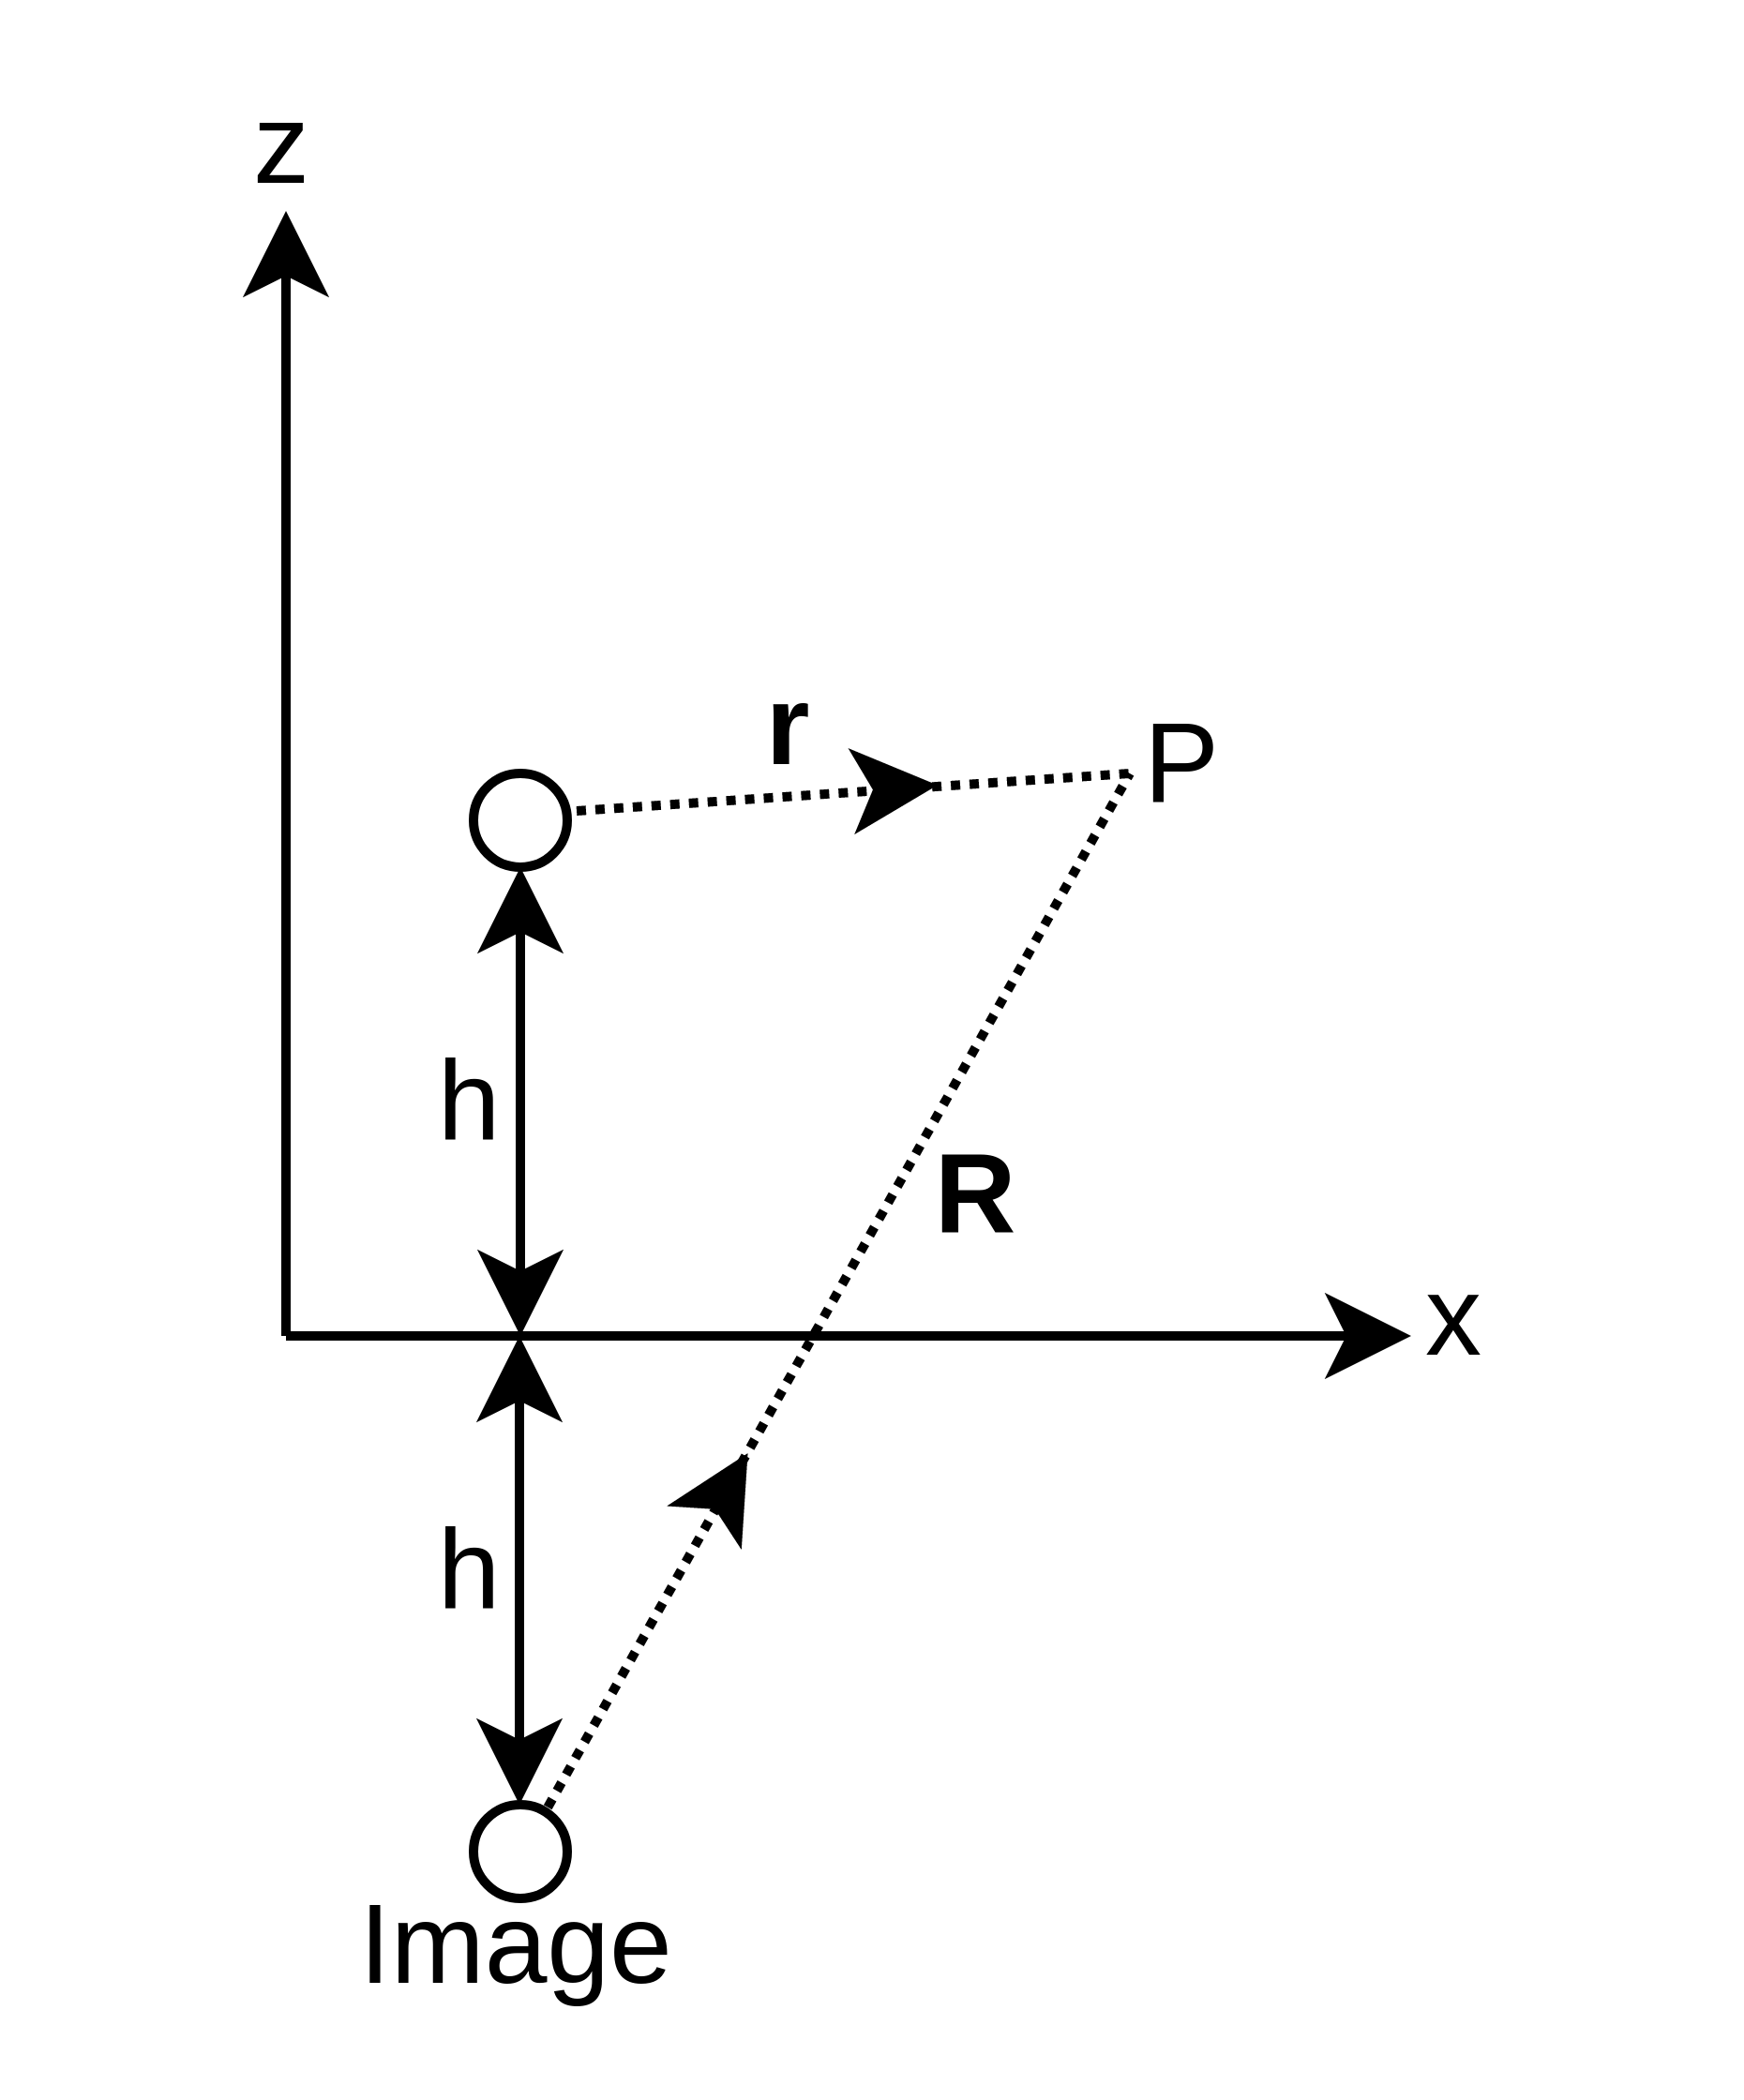
\includegraphics[width=0.7\textwidth]{images_other/blake_reproduction.png}
    \caption{The image system that underpins the Blake tensor. The real Stokeslet is a distance $h$ above the no-slip boundary at $z=0$, and the image system is found a distance $h$ below the boundary. $P$ is the observation point at which we want to compute the flow.}
    \label{fig:blake_image_system}
\end{figure}

This can be rewritten as a Stokeslet plus an `image' contribution:
\begin{equation}
    u_j(\mathbf{r}, \mathbf{R}) = (\mathcal{S}_{jk} + \mathcal{B}^\text{im}_{jk}) F_k.
\end{equation}
The image contribution decays to zero if the particle is far enough from the boundary.

\begin{figure}
    \captionsetup[subfigure]{format=subcap}
    \centering
    \begin{subfigure}[t]{0.45\linewidth}
        \centering%
        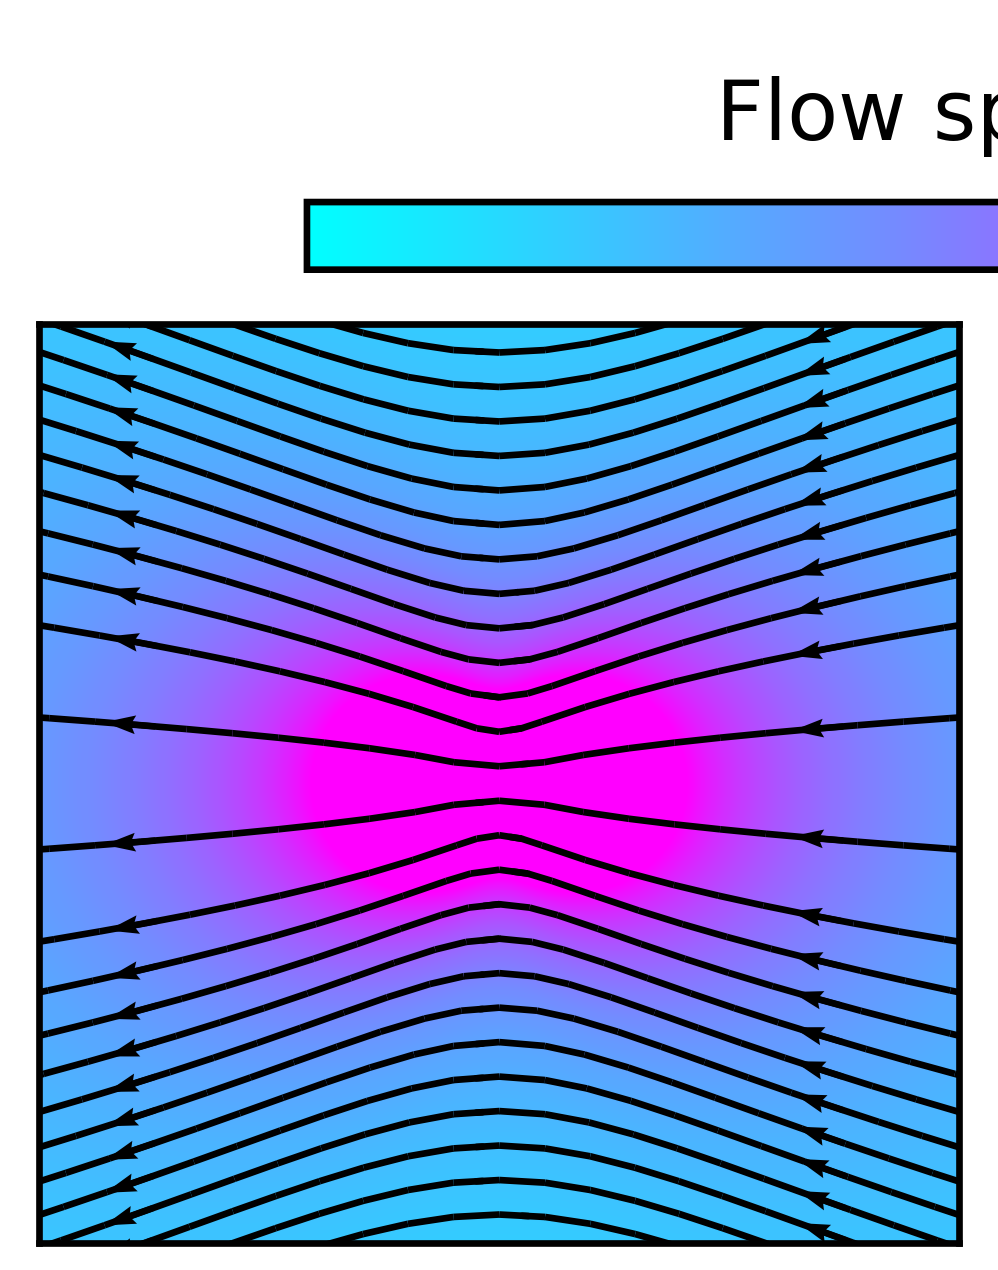
\includegraphics[width=\textwidth]{images_other/stokes_flow_left.png}%
        \caption{Stokes flow due to a moving Stokeslet}%
        \label{fig:flow_sphere_blake}%
    \end{subfigure}%
    \hspace{-20000sp}%
    \begin{subfigure}[t]{0.45\linewidth}%
        \centering%
        \raisebox{10000sp}{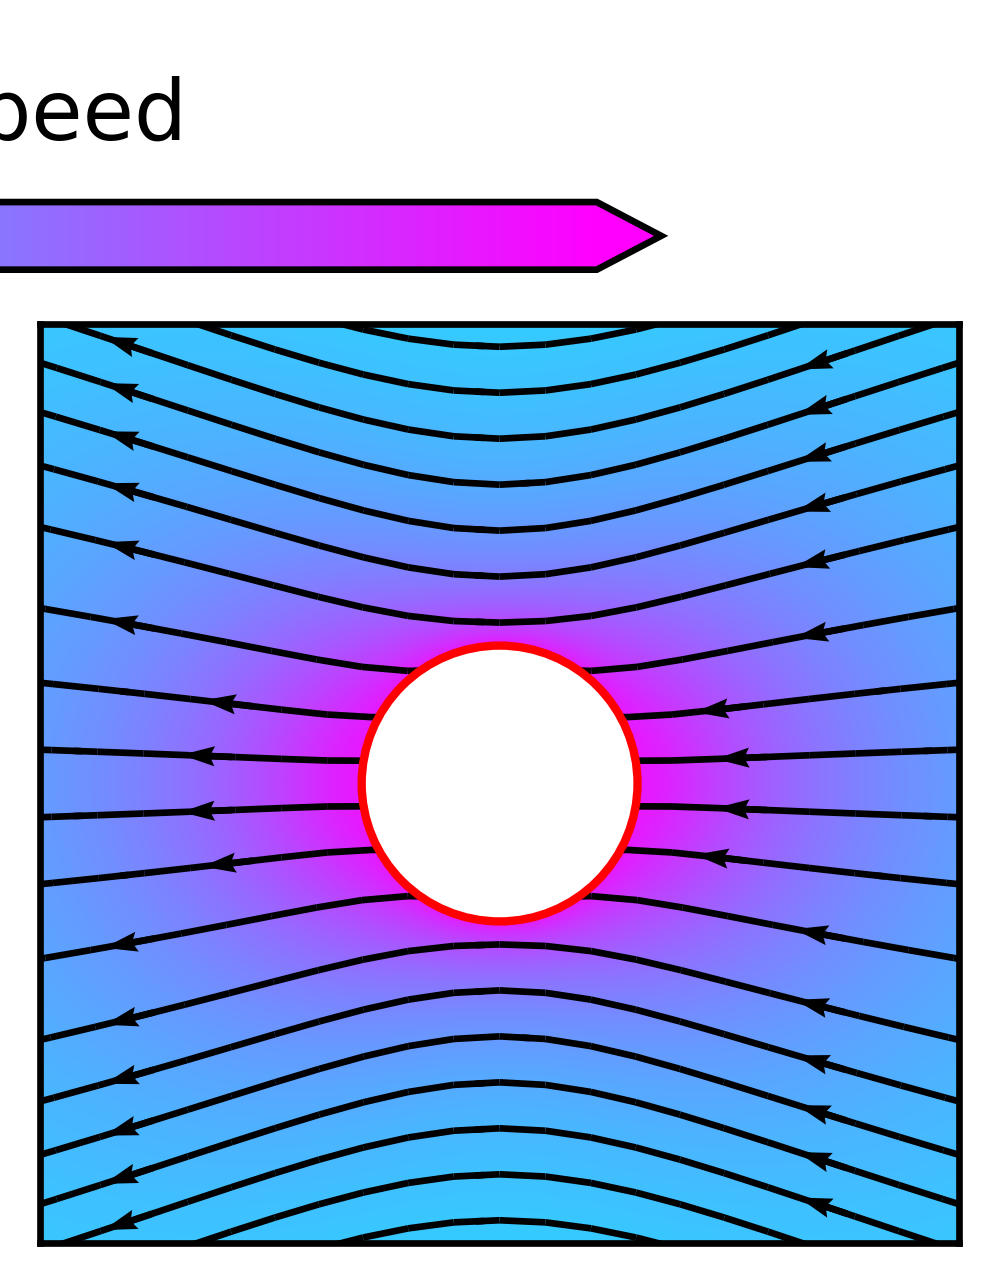
\includegraphics[width=\textwidth]{images_other/stokes_flow_right.png}}%
        \caption{Stokes flow due to a finite-sized sphere}%
        \label{fig:flow_sphere_rp}%
    \end{subfigure}
    
    \begin{subfigure}[t]{0.45\linewidth}
        \centering%
        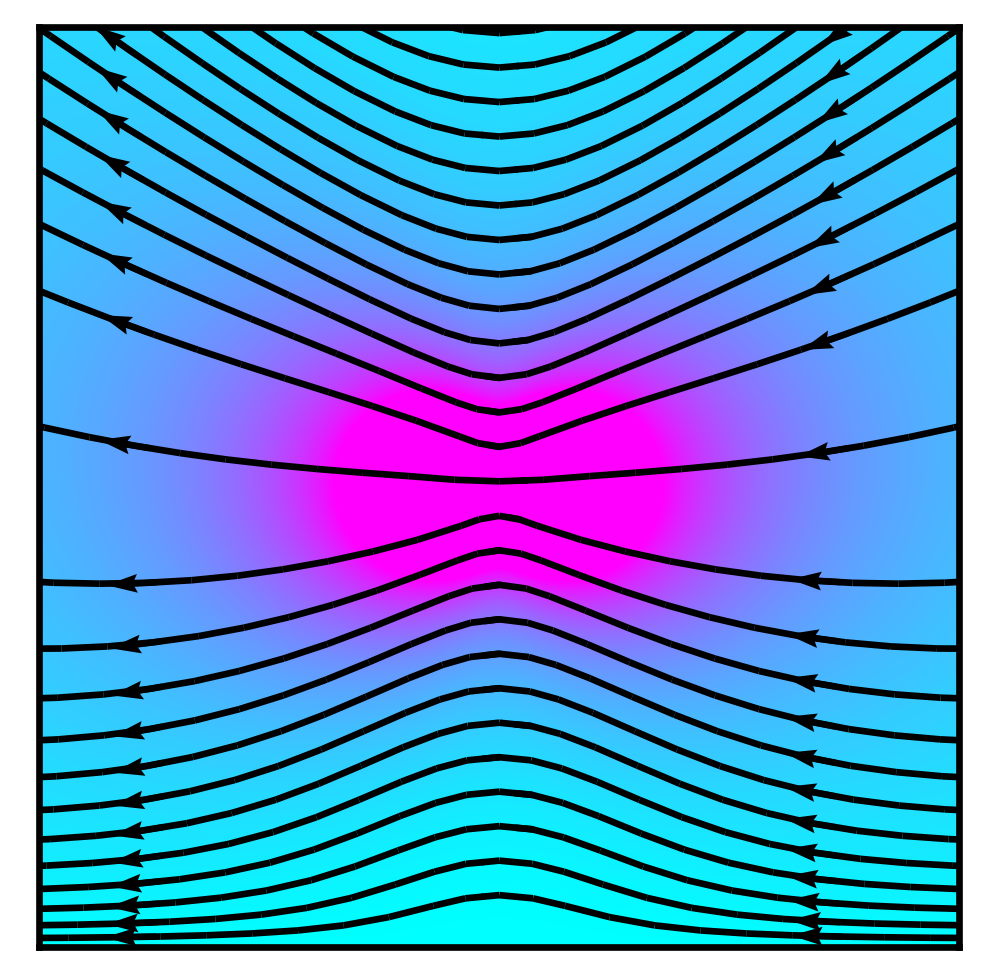
\includegraphics[width=\textwidth]{images_other/stokes_flow_bottomleft.png}%
        \caption{Flow due to a moving Blakelet near a boundary}%
        \label{fig:flow_sphere_blake_bc}%
    \end{subfigure}%
    \hspace{-20000sp}%
    \begin{subfigure}[t]{0.45\linewidth}%
        \centering%
        \raisebox{10000sp}{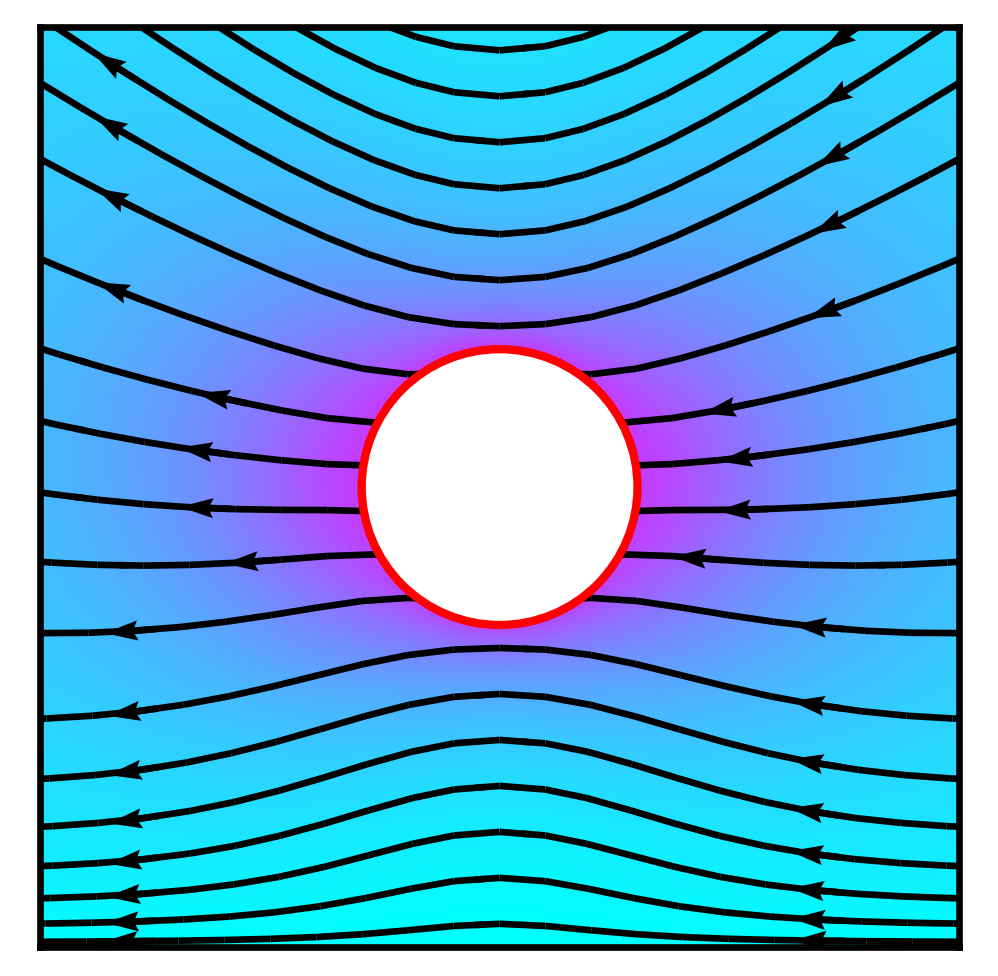
\includegraphics[width=\textwidth]{images_other/stokes_flow_bottomright.png}}%
        \caption{Flow due to a moving finite-sized sphere near a boundary}%
        \label{fig:flow_sphere_rp_bc}%
    \end{subfigure}
    \caption{Different solutions to the Stokes equations corresponding to various Green's functions. (a) and (b) show the flows far away from a boundary, whereas (c) and (d) show the flow field near a no-slip boundary. One can see how the fluid is much slower near the boundary at the bottom edge of the plots, and how the fluid flow is altered.}
    \label{fig:flow_sphere}
\end{figure} % TODO: entire thing in lab frame might make more sense, i.e replace top left and drop top right.

Far away from the cilium, the Blakelet is a very good approximation for the fluid flow due to a moving sphere or even a whole cilium, despite assuming a single point force -- in fact, in the far-field\boxedsidenote[][-100pt]{`Far-field' refers to the fluid behaviour far from the cilium, where only the terms in the force response that decay very slowly with distance are important. `Near-field' refers to the fluid behaviour much closer to the cilium, where the higher order terms are also relevant.} limit, it is exactly the same as the flow due to a sphere acted upon by a force~\sidecite[80pt]{vilfan_generic_2012}. However, closer to the cilium, something more accurate is required; to achieve this, we can integrate the Blakelet over the surface of a sphere of radius $a$ to obtain a version of the Rotne-Prager tensor, modified to include a no-slip boundary. This new mobility satisfies the no-slip boundary on the surface of the sphere. The Rotne-Prager tensor can be written in terms of the Blake tensor as:
\begin{equation}
    \mathcal{M}_{jk} = \left( 1 + \frac{a^2}{6}\nabla^2_{\mathbf{r}_j} \right) \left( 1 + \frac{a^2}{6}\nabla^2_{\mathbf{r}_k} \right) \mathcal{B}(\mathbf{r}_j, \mathbf{r}_k)\label{eq:rp_offdiag}
\end{equation}
for the off-diagonal elements, and
\begin{equation}
    \mathcal{M}_{jj} = \frac{1}{6\pi\mu a}\mathbb{1} + \left( 1 + \frac{a^2}{6}\nabla^2_{\mathbf{r}_j} \right) \left( 1 + \frac{a^2}{6}\nabla^2_{\mathbf{R}_j} \right) \mathcal{B}^\text{im}(\mathbf{r}_j, \mathbf{R}_j)\label{eq:rp_diag}
\end{equation}
for the diagonal elements~\sidecite{gauger_fluid_2009}. The full form of the tensor is much too long to write here, but see for example \etalcite{vilfan_self-assembled_2010}. Some of the fluid flow solutions discussed here are shown in Fig.~\ref{fig:flow_sphere}. Our work in later chapters will make extensive use of this corrected Rotne-Prager tensor.

\FloatBarrier

\nosidecite{gauger_fluid_2009,guazzelli_physical_2011}%\todo{I think we basically neglect F for the offdiagonal terms because it's a higher order contribution; to lower order the sphere is force-free. This doesn't apply to the diagonal case, so we get this eta stuff. But ask Andrej!}
\begin{kaobox}[title=Rotne-Prager derivation]
    The Rotne-Prager tensor can be derived (following~\cite{gauger_fluid_2009}) by integrating the Blakelet over the surface of a sphere of radius $a$ and its centre at $\mathbf{r_s}$:
    \begin{equation}
        \mathbf{u}(\mathbf{r}) = \int_S \mathcal{B}(\mathbf{r}, \mathbf{r}') \mathbf{f}(\mathbf{r}') \, \mathrm{d}S'.
    \end{equation}
    To first order, the force density $\mathbf{f}$ is just the total force $\mathbf{F}$ divided by the surface area of the sphere, which means that we can expand the force and the Blake tensor around $\mathbf{r}'=\mathbf{r}_s$ to get
    \begin{equation}
        \mathbf{u}(\mathbf{r}) \approx \left[ \left( 1 + \frac{a^2}{6} \nabla^2_{\mathbf{r}'} \right) \mathcal{B}(\mathbf{r}, \mathbf{r}') \right]_{\mathbf{r}' = \mathbf{r}_s} \cdot \mathbf{F}.\label{eq:rpderivation1}
    \end{equation}
    Now, Faxén's law tells us that the velocity of a sphere of radius $a$ experiencing a hydrodynamic force $\mathbf{F}$ in a flow is given by:
    \begin{equation}
        \mathbf{F} = 6\pi\mu a \left[ \left( 1 + \frac{a^2}{6}\nabla^2 \right) \mathbf{u}_0 - \mathbf{u}_\text{s} \right]
    \end{equation}
    where $\mathbf{u}_0$ is the fluid flow that would be at the centre of the sphere if the sphere was not there~\cite{guazzelli_physical_2011}, so we can combine this with Eq.~\eqref{eq:rpderivation1}, eliminating $\mathbf{u}(\mathbf{r})=\mathbf{u}_0$ to find the diagonal and off-diagonal terms of the Rotne-Prager tensor.
\end{kaobox}

\subsection{Modelling the motile cilium}

% \todo{Give a brief overview here: you've got your RFT, SBT, regularised stokeslet, and FEM/BEM. You could afford to spend a paragraph talking about each, then say why you're opting for RPY.}

Slender bodies are of great interest in a lot of fields, especially within biophysics: cilia and the superficially similar bacterial flagella are used for swimming and pumping, and many bacteria or other microorganisms have elongated shapes~\sidecite{borker_slender_2019}. Outside of biophysics, certain materials (both natural and artificial) such as clays~\sidecite{koens_tubular-body_2022} or fibre-reinforced composites~\cite{borker_slender_2019} are composed of elongated components. However, there are some problems when trying to numerically model elongated bodies. For example, the boundary element model divides the body's surface into many small elements and then makes assumptions about the hydrodynamic stress on each element to determine the fluid flow around the cilium~\sidecite{guazzelli_physical_2011}, but since the width of the elongated body is very small, a high resolution (i.e. a lot of surface elements) is required to achieve good accuracy. Then, because the other length scale is much larger, this high-resolution has to be extended over a large area, resulting in heavy performance penalties~\cite{koens_tubular-body_2022}. As such, it comes as no surprise that there are a great many ways to model the hydrodynamics of cilium-like structures that attempt to sidestep these computational pitfalls.

One of the conceptually simplest of these approaches is slender body theory, in which an elongated body is approximated by a line of Stokeslets (and other related flow solutions, in order to enforce a no-slip condition), and the fluid flow is then found by summing over the length of the elongated body~\cite{guazzelli_physical_2011}. This exploits the linearity of the Stokes flow, which means that a superposition of solutions to the Stokes flow is also a valid solution to the Stokes flow. In the case of a series of Stokeslets with position $\mathbf{r}_j$, the total fluid flow at $\mathbf{r}$ would be
\begin{equation}
    \mathbf{u}^\text{total}(\mathbf{r}) = \sum_j \mathcal{S}(\mathbf{r}, \mathbf{r}_j) \cdot \mathbf{F}_j.
\end{equation}
Summing up the velocity responses due to a line of point forces is equivalent to considering the much less tractable case where one must find the velocity response due to a line of forces directly. This approach has seen use in modelling bacterial swimming~\sidecite{lauga_bacterial_2016} and cilium beating~\sidecite{fulford_muco-ciliary_1986}. However, the presence of singularities in the flow can pose problems for numerical integration, and it can be expensive to try to determine the (potentially huge) set of forces required to reproduce a given motion coupled with the boundary condition, so other methods have been developed that try to improve upon the numerical practicality. %However, this approximation makes the assumption that the aspect ratio of the body tends to infinity, though it is generally good enough for elongated bodies that are finitely long. 

Other approaches include the numerically much simpler resistive force theory, in which the slender body is divided into (usually infinitesimal) length elements. The force components on each length element are computed using drag coefficients which are known in advance, and the velocity of the length element relative to the fluid at infinity. However, this approximation does not account for self-interaction, so tightly curved filaments can pose issues, and it begins to break down if the slender body is anchored to a much larger cell body (which is almost always the case with cilia)~\sidecite{johnson_flagellar_1979}. Nonetheless, this method has seen success in modelling of ciliary hydrodynamics~\sidecite{gueron_ciliary_1992}. The method of regularised Stokeslets seeks to fix the issues created by the singularities in slender body theory, by replacing each Stokeslet point-force with a `blurry' force distribution called a regularised Stokeslet; the Dirac delta function that characterises the point force is instead replaced by a smooth approximation called a `cut-off' function, which solves the problems introduced by flow singularities. However, there is an issue with `leaking' whereby the no-slip boundary condition is not very well satisfied, which might prove fatal depending on the requirements of the model~\sidecite{cortez_regularized_2018}. Nonetheless, this method has also been applied to cilia~\sidecite{smith_boundary_2009, pedley_hydrodynamic_1992}. Various other methods have been developed, such as the recent tubular-body-theory developed by~\citeauthor*{koens_tubular-body_2022}~\sidecite{koens_tubular-body_2022}.

% \todo{rethink this bit}

However, there is a simpler way to solve the issues arising from flow singularities, which is to avoid creating any in the first place. The primary method we use in this work is to replace the cilium with a sphere or chain of non-overlapping spheres as appropriate, depending on the requirements of the model. 

In Ch.~\ref{ch:results_particle}, where the near-field flow extremely close to the cilium is of great relevance, we approximate the cilium as a chain of beads. Exploiting the linearity of the Stokes flow, we can superpose the flow solution given by the modified Rotne-Prager mobility tensor for each individual sphere, and hence compute the flow due to a chain of spheres in the presence of a no-slip boundary. This is both numerically efficient and a very good approximation to a cilium, even in the near field, that does not suffer strongly from `leaking' effects. 

In the work we will present in Ch.~\ref{ch:results_sync}, we are less concerned with the fluid flow very close to the cilium. Even a single sphere is a good approximation in the far field, and by putting it on a titled circular trajectory, the asymmetry between the power and recovery stroke is reproduced. This is an extremely effective simplification that allows for a great improvement in computational efficiency, which is necessary due to the large numbers of interacting cilia we must simulate.



\section{Cilia}

Cilia are hairlike organelles found on the surface of most eukaryotic cells~\sidecite[-120pt]{nachury_establishing_2019} and certain microorganisms such as \textit{Paramecium}. They can be broadly divided into two types: primary cilia, which do not move under their own power, and motile cilia, which do.

Primary cilia (imaged in Fig.~\ref{fig:sem_primary}) usually have roles in sensing, normally of mechanical forces or chemicals: primary cilia on bone cells detect mechanical stresses~\sidecite{mcglashan_localization_2006}, primary cilia in the kidneys and blood vessels detect fluid flow~\sidecite{goetz_endothelial_2014, nauli_endothelial_2008}, many chemical signals such as serotonin are mainly detected by cilia~\sidecite{brailov_localization_2000}, and even the olfactory receptors in the human nose are primary cilia~\sidecite{marshall_cilia_2006}. Modified primary cilia also sense light~\sidecite{insinna_intraflagellar_2008} and temperature~\sidecite{kuhara_temperature_2008}. All of this sensing ability gives them their nickname of the `cell's antenna'~\sidecite{malicki_cilium_2017}. In fact, nearly every cell in the human body has exactly one primary cilium. Since they are found on most cell types, it is no surprise that they are found in many different tissues, or that when defective, they can cause a large number of diseases (including \textit{situs inversus}) known as ciliopathies~\sidecite{waters_ciliopathies_2011}.

%\boxedsidenote{Blood cells are an obvious exception that have zero primary cilia per cell. Similarly, olfactory cilia are considered primary cilia, but are found with many to a cell.}

\begin{figure}
    % \captionsetup[subfigure]{format=subcap}%
    \centering%
    \begin{subfigure}[t]{0.47\linewidth}%
        \centering%
        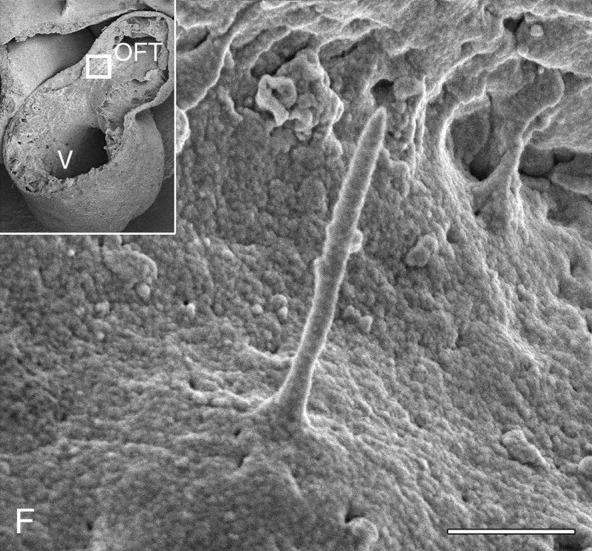
\includegraphics[width=\textwidth]{images_other/primary_cilium.jpg}%
        \caption{Primary cilium in a developing chicken heart. Image from~\citeauthor*{van_der_heiden_monocilia_2006}~\cite{van_der_heiden_monocilia_2006}. Reproduced here with permission of the copyright holder via Rightslink. © 2005 Wiley-Liss, Inc.}%
        \label{fig:sem_primary}%
    \end{subfigure}%
    \hfill
    \begin{subfigure}[t]{0.47\linewidth}%
        \centering%
        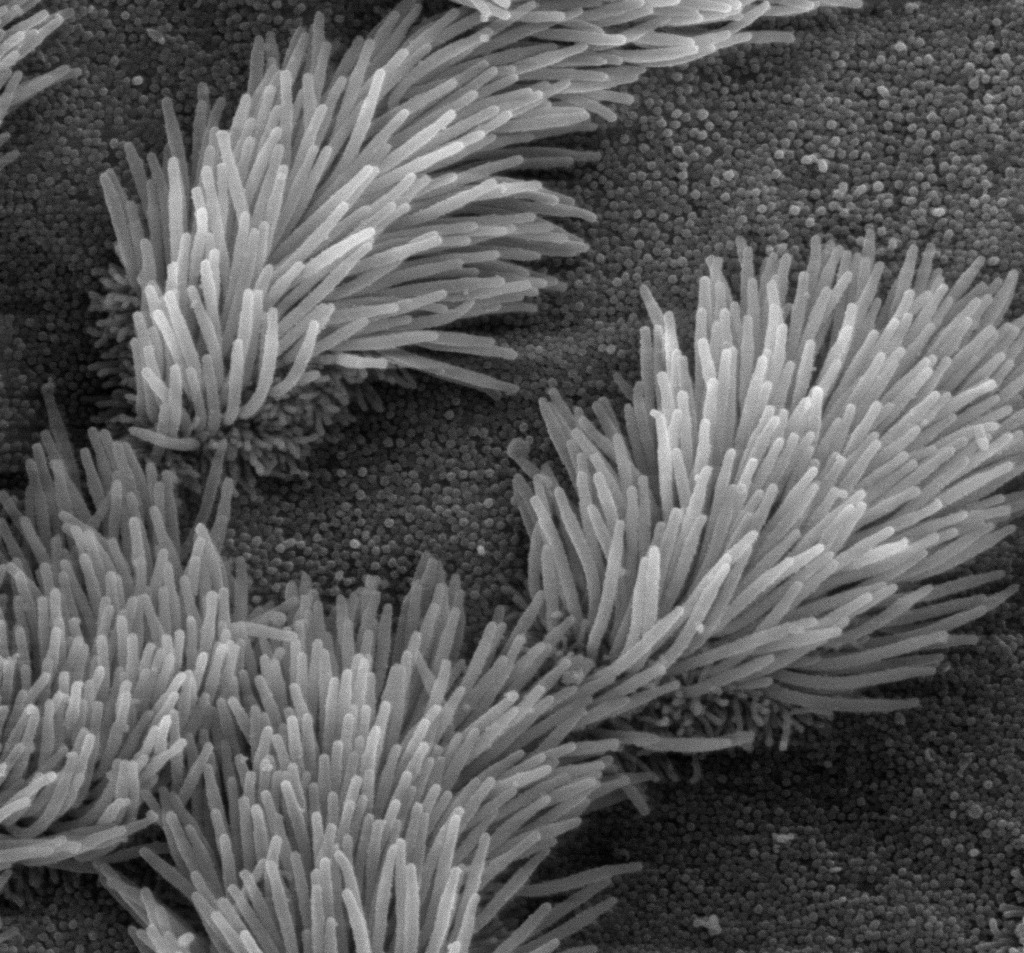
\includegraphics[width=\textwidth]{images_other/trachea_cilia_daghlian_pd.jpg}%
        \caption{Motile cilia in the human trachea. Image by Charles Daghlian and released to the public domain.}%
        \label{fig:sem_motile}%
    \end{subfigure}%
    \caption{Scanning electron microscope images of a single primary cilium (a) and bundles of motile cilia (b). The primary cilium stands alone whereas the motile cilia are found in bundles, which is typical for the two types.}%
    \label{fig:sem_photos}%
\end{figure}

Motile cilia, on the other hand, mostly have roles in fluid pumping, though recent research has also revealed that they have sensory capacity as well~\sidecite{bloodgood_sensory_2010}; this revelation is examined in much more detail in Ch.~\ref{ch:results_particle}. They are usually found in `bundles' or `carpets', where one cells hosts many cilia (imaged in Fig~\ref{fig:sem_motile}); for example, in the lungs, multiciliated cells have around 200 cilia per cell~\sidecite{horani_advances_2018}. They are also found in many places in the body: as previously mentioned, they are found in the lungs and trachea~\sidecite[-30pt]{yaghi_airway_2016}, where their waving works to move mucus out of the lungs to remove trapped pathogens and particulates. They are also found pumping fluid in the brain to move signalling molecules~\sidecite[-60pt]{olstad_ciliary_2019}, in the reproductive system (both male~\sidecite[-43pt]{yuan_motile_2019} and female~\sidecite[-5pt]{lyons_reproductive_2006}) and on the surface of microscopic organisms where they help with feeding and swimming~\sidecite{funfak_paramecium_2015, mannan_minimal_2020}. As with primary cilia, defective motile cilia lead to a large number of diseases~\sidecite{afzelius_cilia-related_2004}.

The beat of a motile cilium is asymmetric and irreversible, meaning that the problem posed by scallop theorem is avoided. The beat begins with a straightened cilium performing a power stroke, intended to move as much fluid as possible as fast as possible. The cilium then curls up and returns to its original position in a so-called recovery stroke, staying as close to the cell surface as possible~\sidecite{gueron_energetic_1999}. Due to the curled-up shape of the recovery stroke, and the no-slip condition on the cell surface, the cilium doesn't move much fluid during the recovery stroke compared to the amount moved during the power stroke, giving a net pumping effect. This beating pattern is illustrated in Fig.~\ref{fig:motile_beat}. At sufficient density, motile cilia can coordinate their beating to improve their efficiency and minimise intercilium collisions~\sidecite{osterman_finding_2011, ringers_novel_2023}; the mechanisms underpinning this behaviour are examined in Ch.~\ref{ch:results_sync}.

\begin{figure}
    \centering
    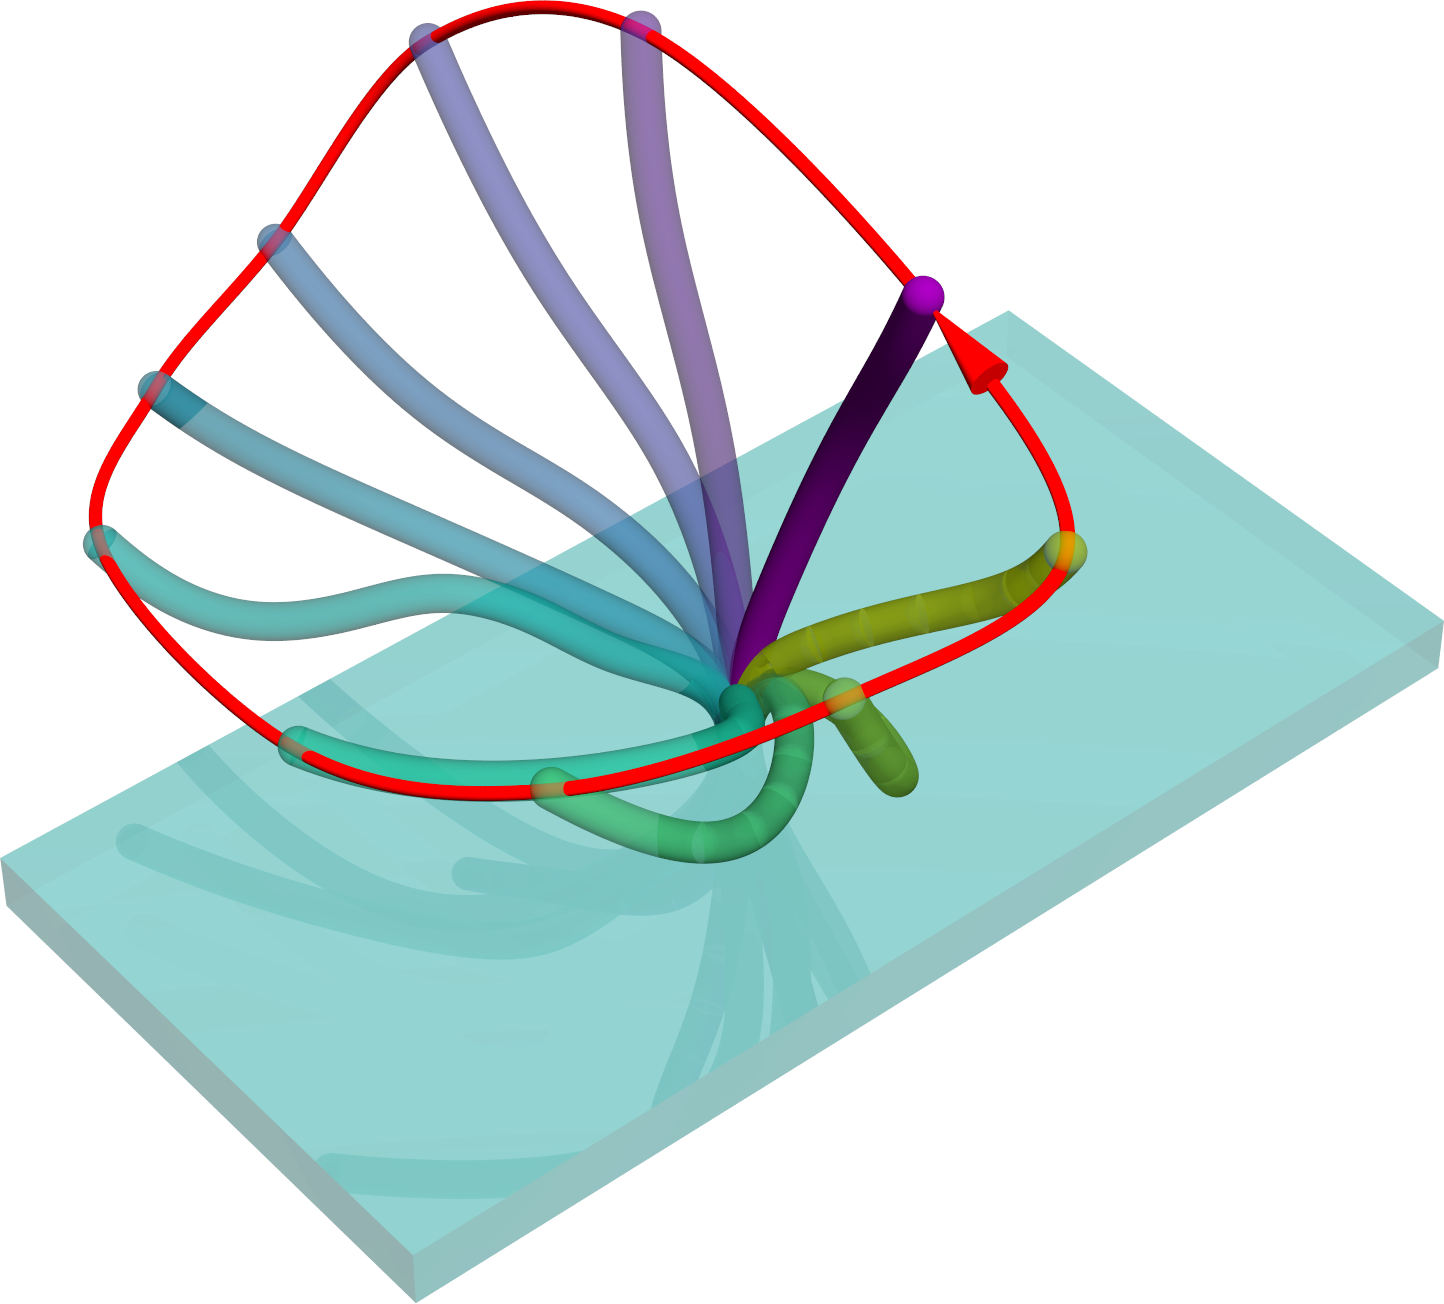
\includegraphics[width=0.6\linewidth]{images_other/enhanced_motilebeat.png}
    \caption{Motile cilium beat. The cilium performs a power stroke (solid dark blue colour), then curls up and pulls back along the cell surface. The trajectory breaks time reversal symmetry, so it can produce a net flow without falling afoul of scallop theorem.}
    \label{fig:motile_beat}
\end{figure}

Both primary and motile cilia consist of a basal body affixed to the cell, and a protruding structure with a microtubule skeleton, all covered in cell membrane. The basal body works to organise and support the microtubules. The microtubule `skeleton' of the cilium is called the axoneme, and consists of a series of nine microtubule doublets, shown in Fig.~\ref{fig:axoneme}a-b for the two cilium types. The primary cilium and the motile cilium have slightly different axonemes: the motile cilium has an additional pair of microtubules in the centre (hence the name 9+2 axoneme, for the nine outer doublets and the two inner microtubules), and some radial spokes that connect it to the outer doublets, along with some dynein arms that are responsible for sliding the microtubules relative to one another to generate bending~\sidecite{falk_specialized_2015}. The primary cilium lacks the central pair of microtubules, leading to it being named a 9+0 axoneme, as well as lacking the dynein arms and radial stokes. The structure of the motile cilium, including the additional apparatus required for motility, is shown in cross-section in Fig.~\ref{fig:axoneme_motile_2d}.

There are, however, exceptions to this seemingly neat classification: in the structure responsible for the left-right differentiation of mammalian embryos (creatively named the left-right organiser), specialised motile cilia (called `nodal cilia') lack the central pair, and they have a very different (and simpler) beating pattern compared to regular motile cilia. Kinocilia, found in the inner ear, have a 9+2 axoneme, like motile cilia, but they don't have the dynein arms and they don't move under their own power; they simply bend under the influence of external vibrations, and are usually considered to be a variant of primary cilia. There can therefore be said to be four types of cilia depending on the combination of axoneme type and motility~\cite{falk_specialized_2015}.

\begin{figure*}
    \begin{subfigure}[t]{0.49\linewidth}
        \centering
        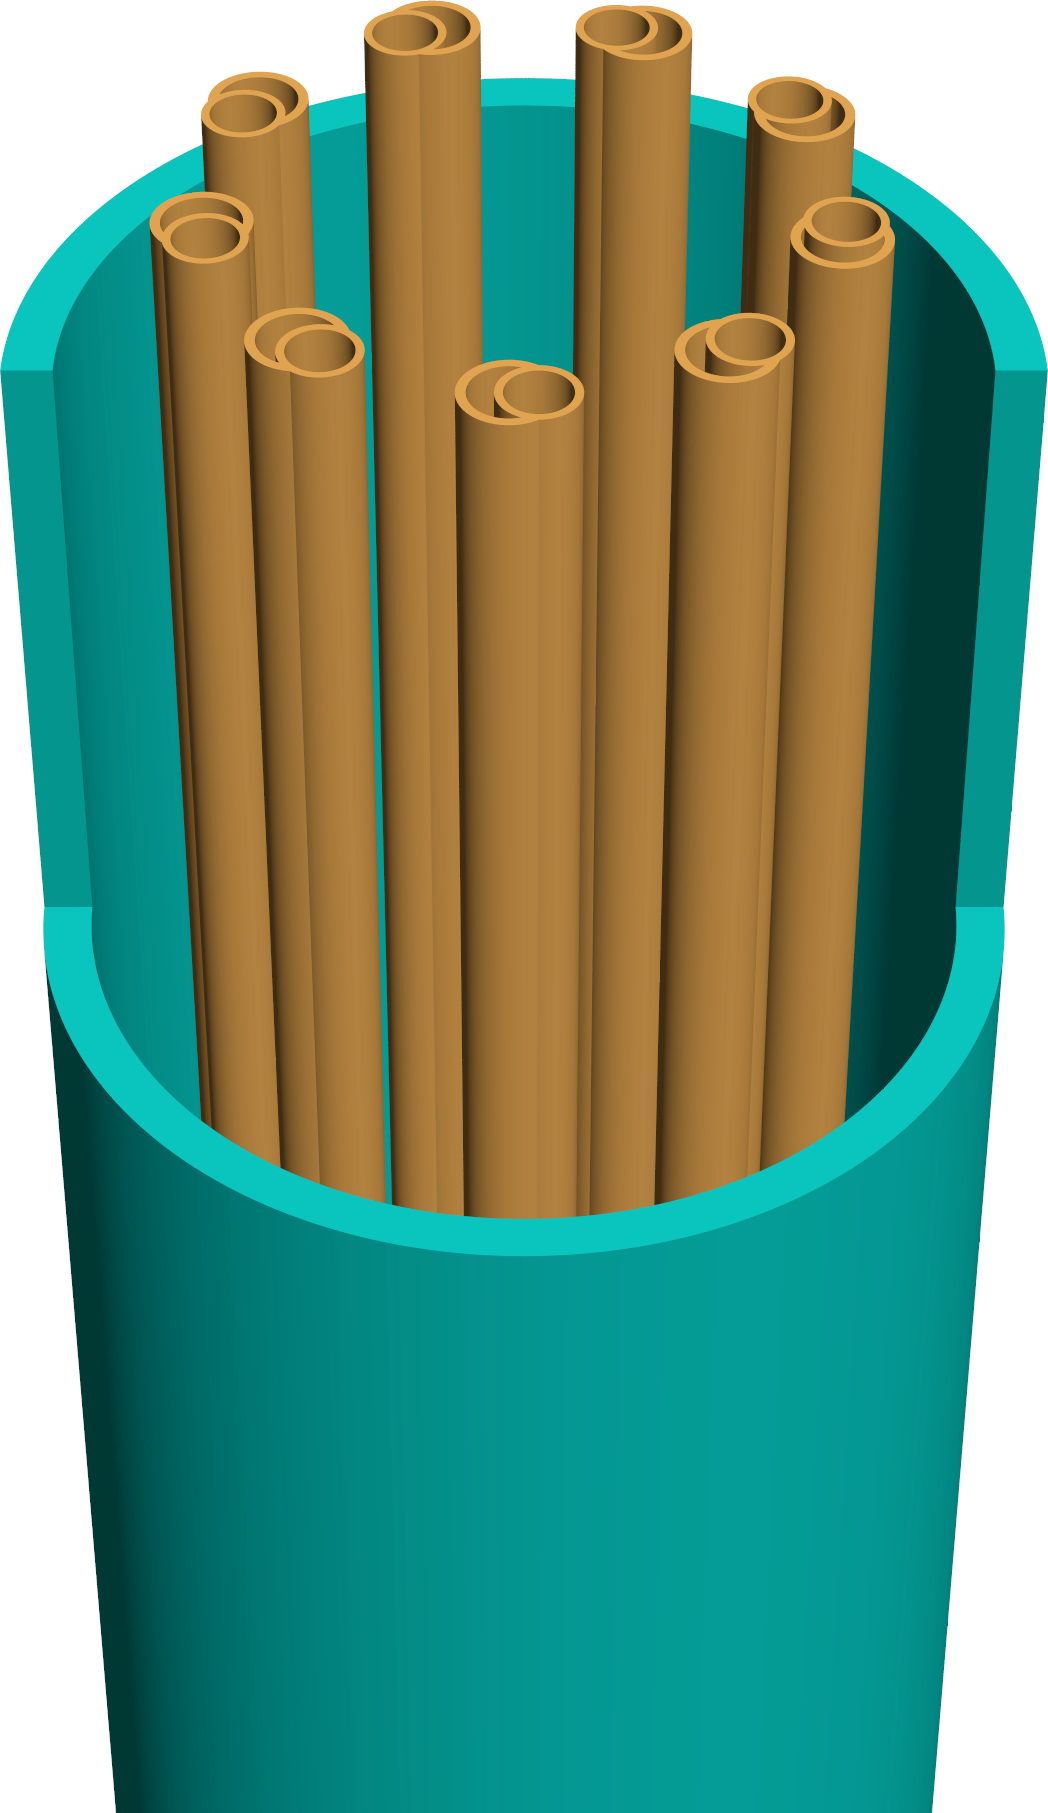
\includegraphics[width=0.50\textwidth]{images_other/enhanced_axoneme.png}
        \caption{Render of the microtubule structure of a primary cilium. Because it has nine doublets and no central pair, this arrangement is often referred to as a 9+0 axoneme.}
        \label{fig:axoneme_primary}
    \end{subfigure}
    ~
    \begin{subfigure}[t]{0.49\linewidth}
        \centering
        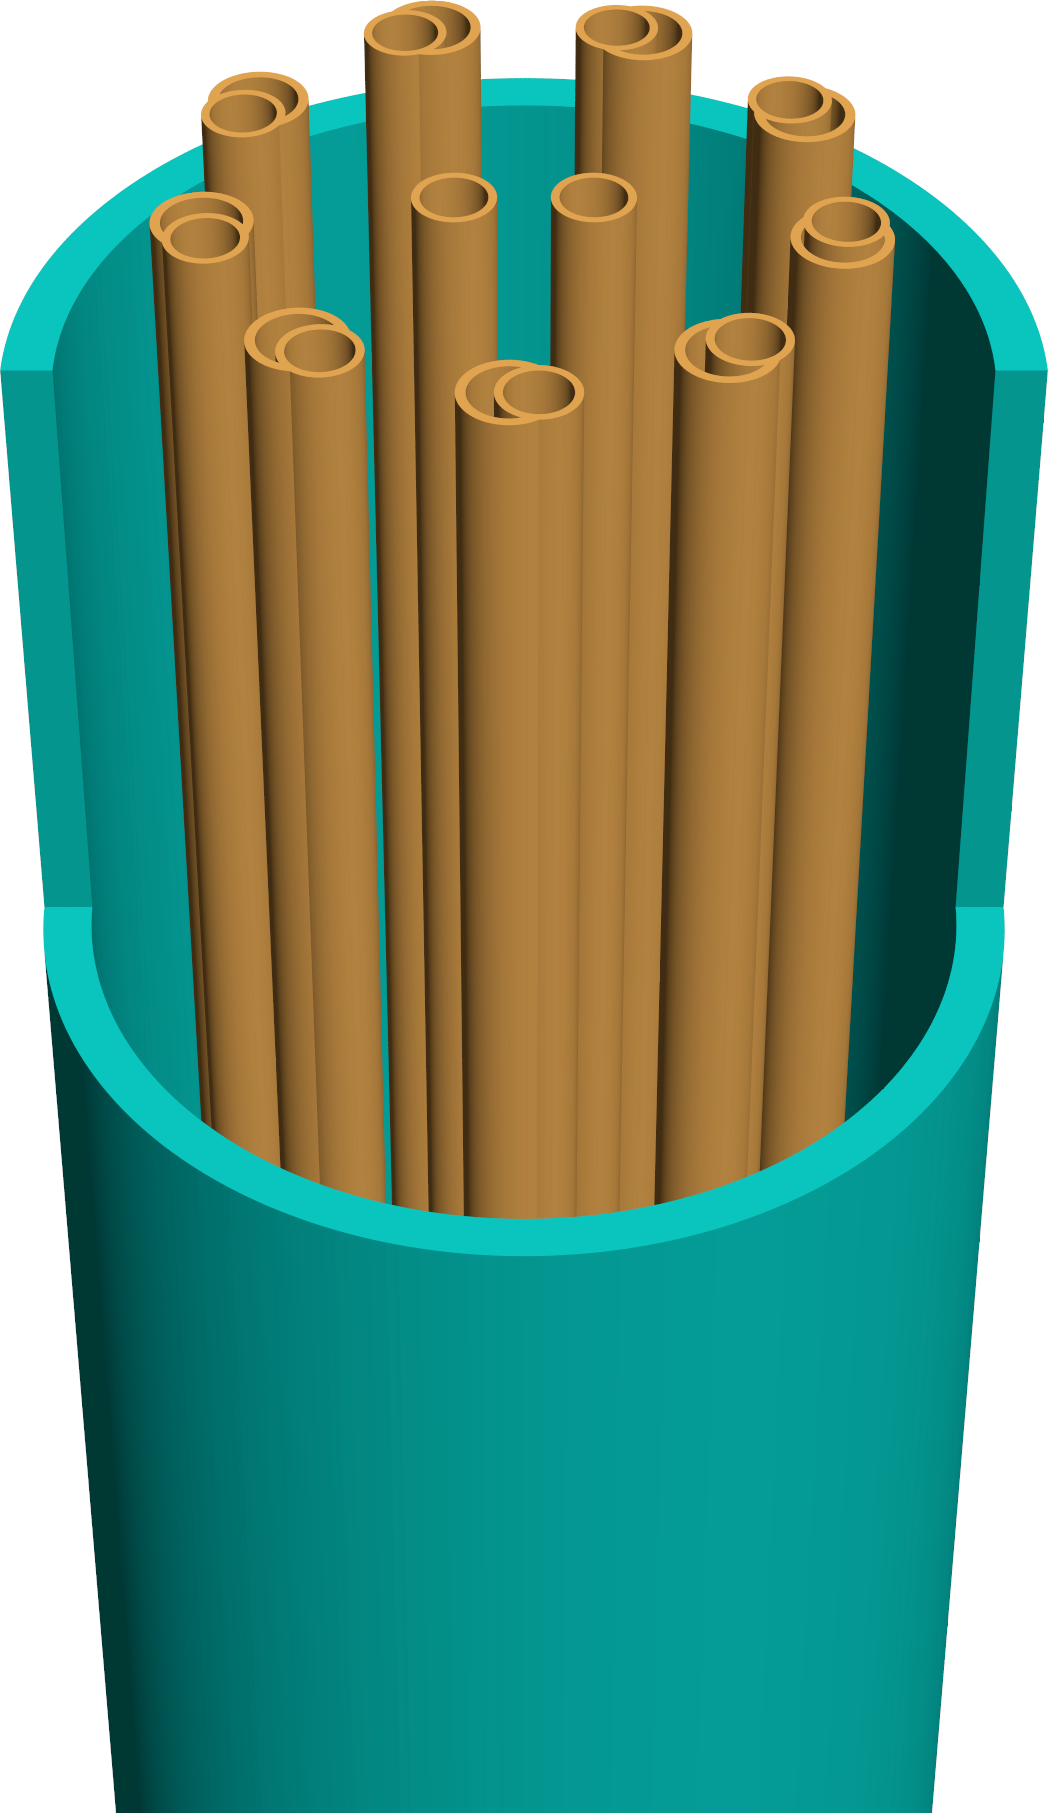
\includegraphics[width=0.50\textwidth]{images_other/enhanced_axoneme_motile.png}
        \caption{Render of the microtubule structure of a motile cilium; note the two central microtubules (which are absent in the primary cilium case) which along with the nine doublets give this axoneme arrangement its designation as a 9+2 axoneme.}
        \label{fig:axoneme_motile}
    \end{subfigure}
    
    \begin{subfigure}[t]{0.49\linewidth}
        \centering
        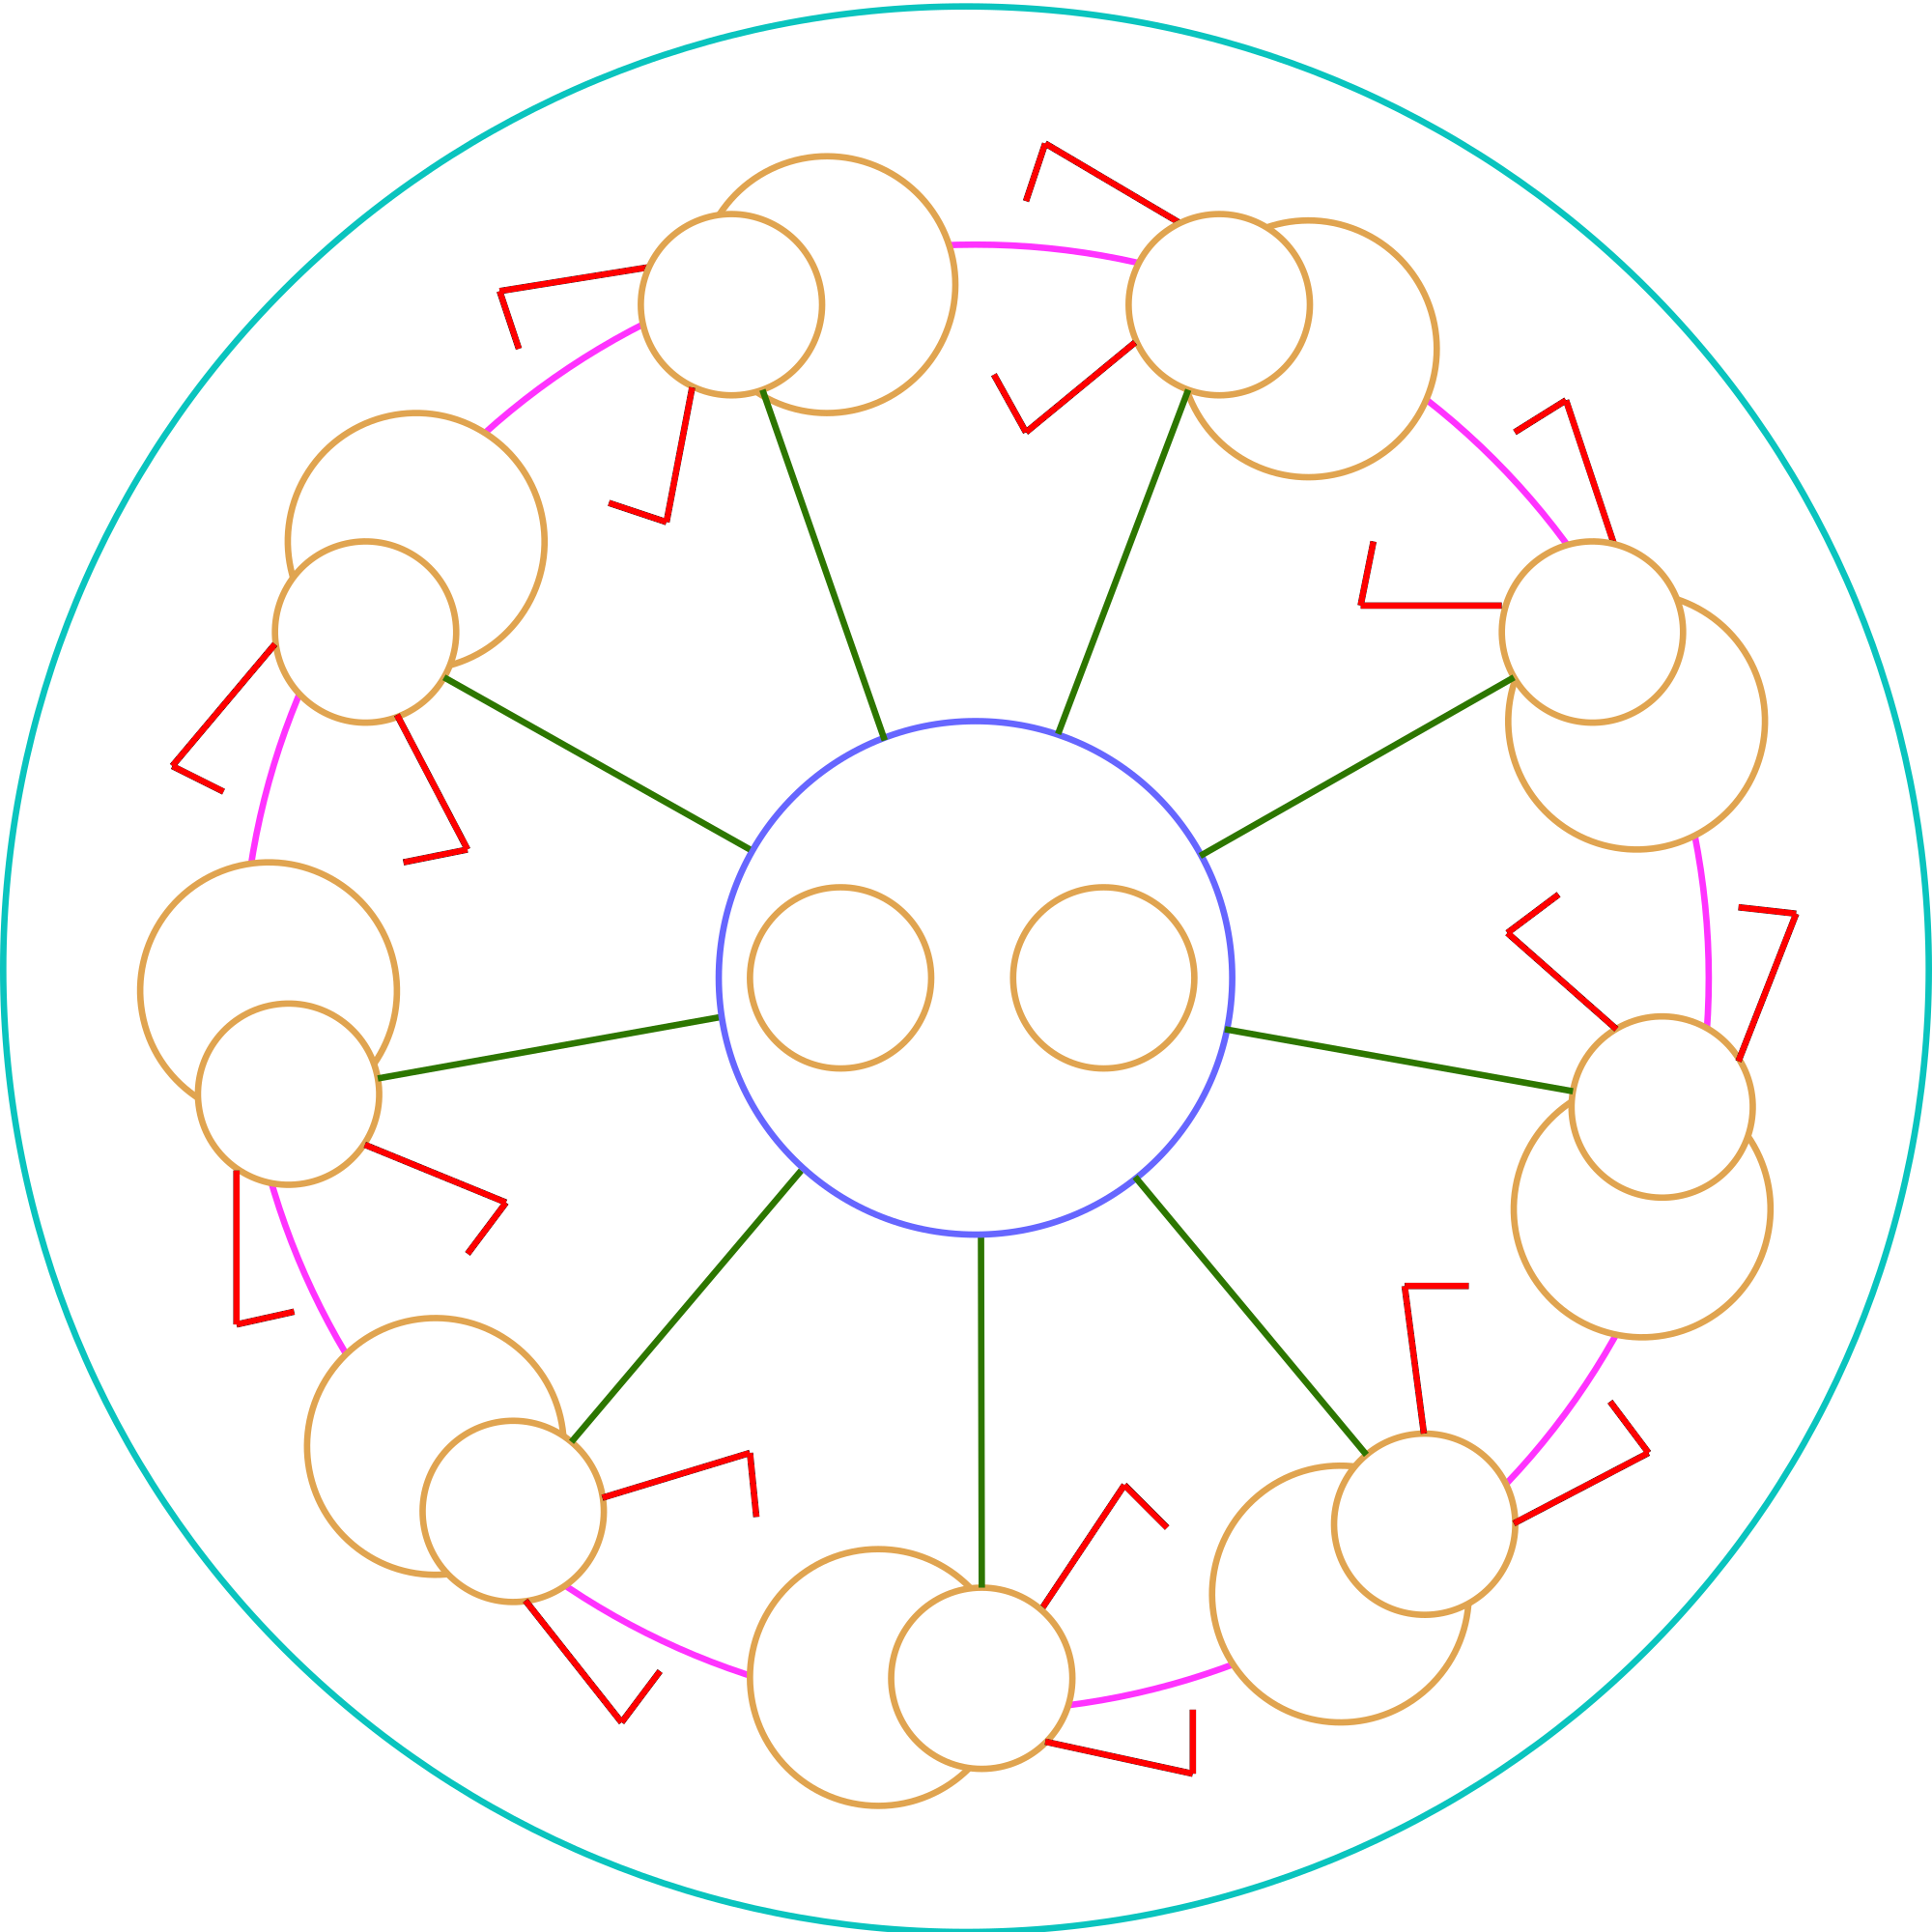
\includegraphics[width=0.8\textwidth]{images_other/axoneme_2d.png}
        \caption{Top-down view of motile cilium axoneme. The outer tubule doublets and central microtubules (yellow) are visible, along with the spokes connecting them. The dynein arms that give rise to the motility of the cilium are shown in red; these generate sliding motion between the doublets and thus create the cilium's bending motion. The primary cilium lacks almost all of the structure shown in this diagram, except for the outer doublets.}
        \label{fig:axoneme_motile_2d}
    \end{subfigure}
    ~
    \begin{subfigure}[t]{0.49\linewidth}
        \centering
        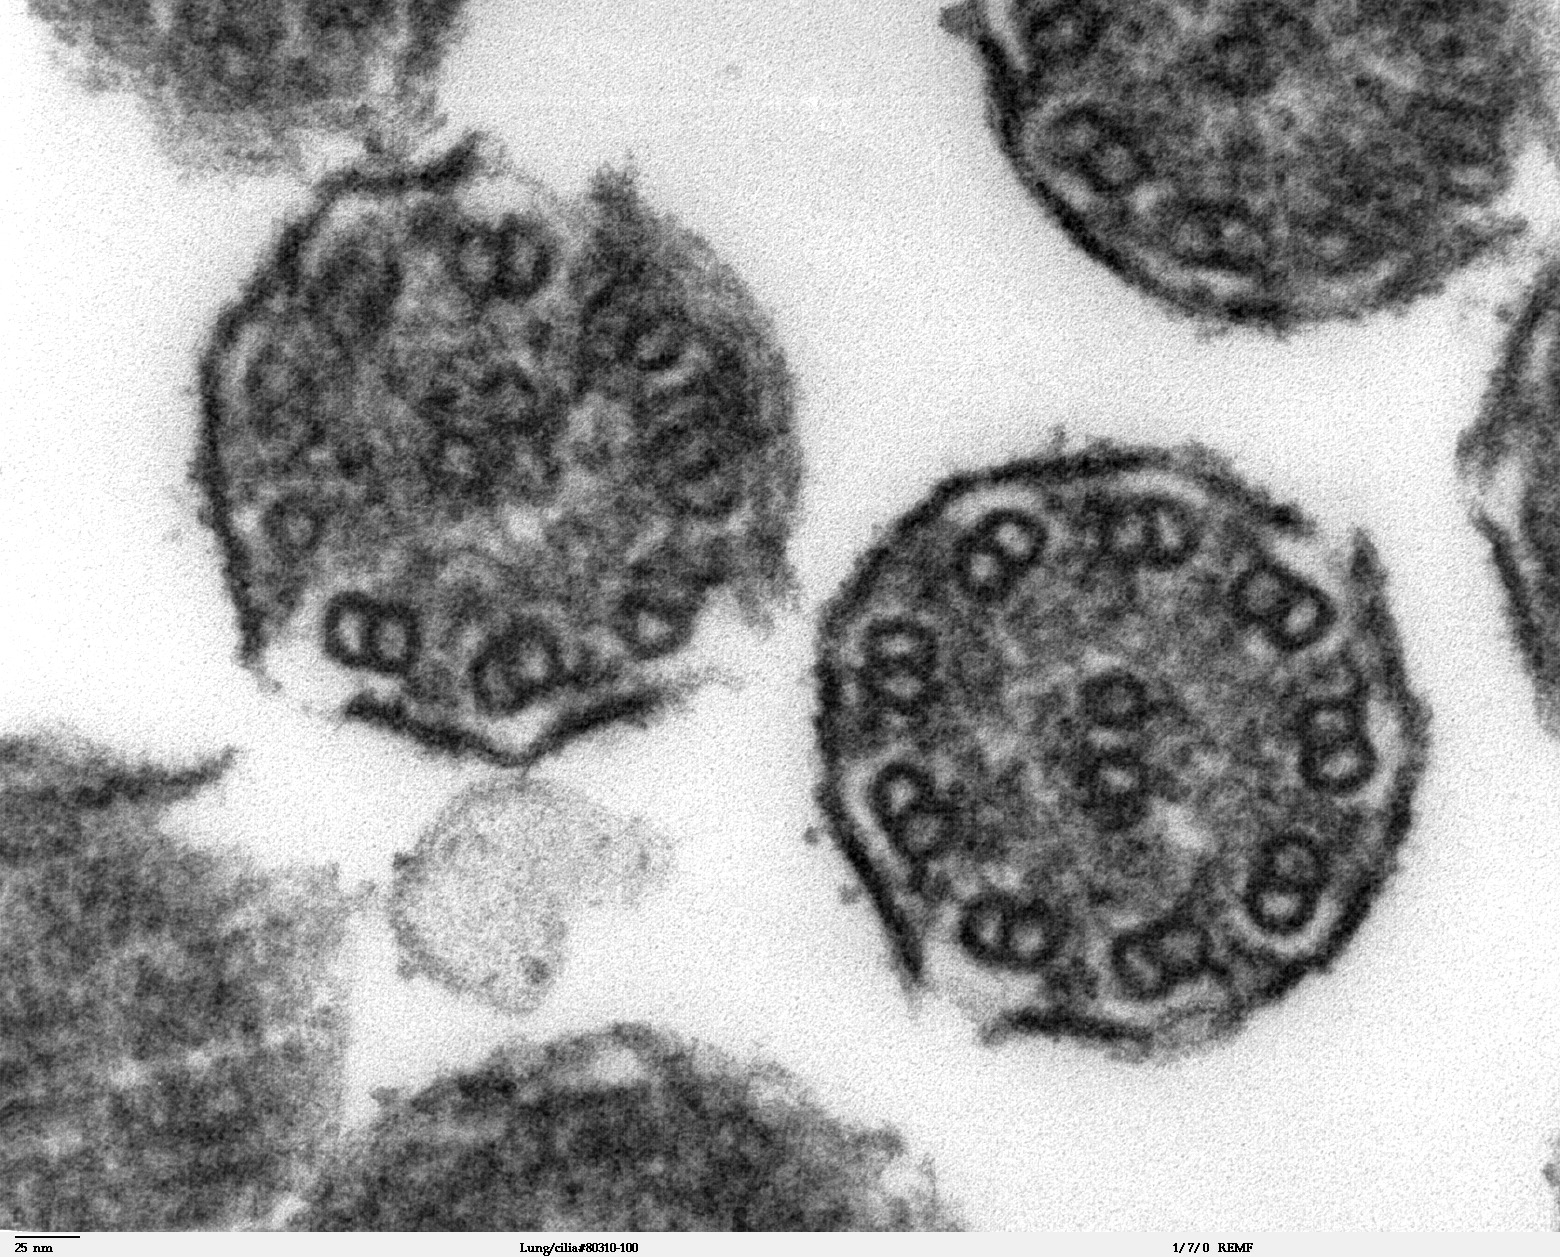
\includegraphics[width=0.9\textwidth]{images_other/lung_cilia_crosssection_howard_pd.jpg}
        \caption{Photo showing the axoneme of some motile cilia in the mammalian lung from above. The doublets are clearly visible, as is the central microtubule pair. Taken by Louisa Howard and released to the public domain.}
        \label{fig:axoneme_sem}
    \end{subfigure}
    
    \caption{Structure of the two types of cilia.}
    \label{fig:axoneme}
\end{figure*}

\section{Chapter summary}

\begin{itemize}
    \item At the length scale of cilia, fluid behaviour is dominated by viscosity, which greatly simplifies the equations of fluid motion.
    \item These simplified equations can be solved using various mobility tensors, the most relevant of which is the Rotne-Prager tensor. This approach results in high computational efficiency, even when accounting for no-slip boundaries on the surfaces of spherical bodies, or including planar no-slip boundaries.
    \item The linearity of the Stokes flow permits a lot of approaches to modelling slender bodies, and we favour an approach based on superposing Green's function solutions.
    \item Cilia come in two main types: primary and motile cilia. Both can be chemosensitive but only the motile cilia have roles in pumping.
    \item Motile cilia break time-reversal symmetry with an asymmetric beat consisting of a power and recovery stroke.
\end{itemize}

% Still TODO for this chapter:
% - explicit far field expression for Blake.

\setchapterpreamble[u]{\optmargintoc}
\chapter{Particle capture}
\labch{results_particle}

% 0. Cool hook [1 para]
% Hey, if we start off about sensing more generally, we could stick more closely to the original layout?
The ability to sense chemicals was one the earliest kinds of environment sensing to evolve, and chemosensing abilities are known to be present in organisms spanning all biological kingdoms~\sidecite[35pt]{sokolinskaya_molecular_2020}. Humans have chemosensory abilities, most obviously in the forms of a sense of smell and taste, but in myriad other ways such as detecting blood carbon dioxide level~\sidecite[30pt]{cummins_mechanisms_2020}. For certain microorganisms, chemosensing is integral to their ability to swim along chemical gradients to find nutrients (in a process called `chemotaxis')~\sidecite[40pt]{sarvestani_simulation_2016}. Even plants can sense chemicals in their environment, for example to trigger a response to dangerous pathogens~\sidecite[40pt]{zipfel_plant_2014}. Within organisms, chemosensing is everywhere, for example in the form of signalling chemicals that can convey messages between cells. Chemosensing is therefore an incredibly important facet of life as we know it, and in eukaryotes, many of these chemosensors are found on cilia~\sidecite{marshall_cilia_2006}.

% 1. What is chemosensing? [1 para]
% Kind of covered above...

% 2. Why is it important? 
% Kind of covered above...

% 3. Where does it happen? Specific examples, examined more closely? Does chemosensing underpin other senses? Mention GCPRs near the end, and namedrop cilia (INCLUDING MOTILE CILIA) right at the end of this bit, plus motivate a tiny bit as to why one might not be ultra shocked to find them on cilia. [4+ paras]
When the primary cilium was first discovered, it was widely assumed to be useless and vestigial. A sensory role was first proposed for it at the end of the 19th century~\sidecite{zimmermann_beitrage_1898, bloodgood_sensory_2010}, but it took many years for this idea to be taken seriously, whereupon the primary cilium experienced a huge explosion in popularity. More recently, it was realised that motile cilia are also chemosensory, though the evidence has been piling up for a long time~\cite{bloodgood_sensory_2010}.

Primary cilia have a high density of receptors, in particular G-protein-coupled receptors (often shortened to GPCRs)~\sidecite{mykytyn_g-protein-coupled_2017}. G-proteins are a family of proteins found inside cells, that act as molecular switches. The G-protein-coupled receptors are transmembrane structures that bind to a specific extracellular signalling molecule. This binding causes the GPCR to change its shape (i.e. undergo a conformational change) which affects the shape of the intracellular part of the GPCR, which allows this intracellular part to alter the environment within the cilium~\sidecite{mykytyn_g-protein-coupled_2017}, which can in turn affect the cellular behaviour. It is estimated that close to half of all drugs available target these GPCRs~\sidecite{cheng_luciferase_2010}, so understanding ciliary chemoreception is extremely useful.

% \todo{Read tuning into cell's antenna, it's a very good overview of this paragraph}
There are several reasons why primary cilia have a high chemosensor density: the environment very close to the cell is often not a good representation of the actual intercellular medium, because cells have charged lipids on their surfaces that can repel or attract various chemicals and ions~\sidecite{marshall_cilia_2006}. Many cells are also surrounded by a so-called glycocalyx, a several micrometre thick covering of sugars, lipids, proteins~\sidecite{ebong_imaging_2011} that acts as a physical barrier to protect and control entry to the cell, as well as filling various other roles~\sidecite{reitsma_endothelial_2007}; however, this covering will also alter the chemical environment close to the cell~\cite{marshall_cilia_2006}. The no-slip condition on the cell's surface could also mean that the role of advection very close to the cell's surface is almost totally suppressed, thus limiting fluid mixing and therefore chemosensitivity~\cite{marshall_cilia_2006}. There is also the fact that, because the cilium has a very high surface area to volume ratio compared to the rest of the cell, only a small number of chemosensors and signalling molecules are required to create large changes in the concentration of second messengers\boxedsidenote{These are signalling molecules that are released inside cells in response to some extracellular signalling molecule that is detected by a chemosensor on the cell (or `first messengers').} in the cilium's cytoplasm; by comparison, an enormous number of chemosensors would be required to achieve a similar increase~\cite{marshall_cilia_2006}. Our work aims to see if there are further geometric reasons for placing chemosensors on cilia, as well as determining what advantages arise when combing chemosensing with motility.


% 4. Physics bit! Diffusion, Péclet, diffusion limit, electrostatic analogy. Can cilia break diffusion limit? [4+ paras]
\section{Physics of chemoreception}
In 1827, the famous botanist Robert Brown was looking through his microscope at some grains of pollen in water, and noticed that they were jiggling, moving in seemingly random directions with seemingly random speeds~\sidecite{feynman_feynman_2006}. This random motion, eponymously called Brownian motion, was later used by Albert Einstein to prove the existence of atoms. He (correctly) proposed that this random jiggling was caused by the particles that make up the water, moving around and colliding with the pollen grains. At some times the pollen would be bombarded more on one side than another, giving a net force. Since this bombardment is constantly in flux, the direction of pollen motion changes constantly and unpredictably~\sidecite{einstein_uber_1905}. This random motion will eventually cause chemicals to become spread out and mixed: a drop of ink in a glass of water will eventually diffuse to tint the entire glass equally.

At the scale of cells and cilia, this process of diffusion is extremely fast, with a timescale given by
\begin{equation}
    \tau_D = \frac{L_c^2}{D},\label{eq:diffusion_scale}
\end{equation}
for some characteristic length $L_c$. $D$ is the diffusion constant of the molecule being transported. 
For something the size of a small signalling molecule being absorbed by a cilium, this timescale is of the order of $\sim 0.1$ seconds\boxedsidenote{At the synapses between nerve cells, diffusion carries the signal across the gap junction, a distance of a few tens of nanometres \cite{widrow_chapter_2019}. Since human reaction time is only a few hundred milliseconds, this gives an idea of how fast diffusion can happen.}.\nosidecite{widrow_chapter_2019} 


The dominance of advection over diffusion can be quantified by the dimensionless Péclet number:
\begin{equation}
    \mathrm{Pe} = \frac{L_c v_c}{D}\label{eq:def_pe},
\end{equation}
where a large Péclet number means advection is dominant, and vice versa. Humans barely notice diffusion, so for a human this number is incalculably large, but for something like a signalling molecule close to the no-slip boundary of a cell, this number is much smaller than one. The length scale $L_c$ in the expression for the Péclet number, as well as the fact that $D$ tends to be larger for smaller, lighter particles, means that diffusion is an incredibly powerful force at small scales, and is often the dominant factor in molecular transport~\sidecite{berg_physics_1977}.

This leads neatly to the concept of diffusion-limited reactions. If we have some perfectly reactive body with a surface $S$, such that any particle of interest that touches it is immediately absorbed\boxedsidenote{As shown by \citeauthor*{berg_physics_1977}~\cite{berg_physics_1977}, even if chemosensors only cover 1\% of the area of a body, one still has near-perfect absorption, so this is a surprisingly accurate assumption for real systems.}\nosidecite{berg_physics_1977} (or converted to other molecules, or adsorbed, or otherwise removed from the population of particles) then this can be represented as a boundary condition where the concentration of those particles is zero ($c(\left|\mathbf{r}\right|\in S,t)=0$). Far away from this absorbing body, there is some representative unperturbed concentration $c(\left|\mathbf{r}\right|\rightarrow\infty,t)=c_0$. In the steady state, the advection-diffusion equation, which describes the concentration field, is very simply
\begin{equation}
    D \nabla^2 c(\mathbf{r},t) - \mathbf{u}(\mathbf{r},t)\cdot\nabla c(\mathbf{r},t) =  \frac{\partial c(\mathbf{r}, t)}{\partial t} = 0,
\end{equation}
subject to the boundary conditions above, and where $\mathbf{u}$ is the fluid velocity. Fick's law, which relates the concentration gradient to the average particle flux, means that the rate at which this body absorbs particles can be written as
\begin{equation}
    R = \iint_S \mathrm{d}\mathbf{S}\cdot (D\nabla c).
\end{equation}
$R$ is proportional to $c_0$, but we can define a rate constant $k=R/c_0$ which is independent of the far-field concentration.

In the absence of advection, the diffusion equation reduces to
\begin{equation}
    D\nabla^2 c(\mathbf{r}) = 0,
\end{equation}
which is exactly analogous to the source-free Laplace equation for the potential $\phi$ in electrostatics:
\begin{equation}
    \nabla^2 \phi(\mathbf{r}) = 0.
\end{equation}
It is possible to find the concentration field by finding pre-existing solutions for the electrostatic problem in the scientific literature, as electrostatics is a much more widely-studied field. Alternatively, and as shown in the appendix of the article below, one can show that the self-capacitance $C$ of the body can be straightforwardly converted to a rate constant:
\begin{equation}
    k = \frac{D}{\varepsilon_0} C,
\end{equation}
where $\varepsilon_0$ is the dielectric permittivity of free space.
It is relatively straightforward to adapt this for the case of a particle near a no-slip boundary, using the method of images. One can introduce a second equally-charged `image' particle, reflected in the no-slip boundary, and then compute the self-capacitance (and hence reaction rate constant) of the particle in the presence of its image.

This rate of absorption due to pure diffusion is called the diffusion limit, and puts an upper bound on how fast microorganisms and cilia can detect chemicals in the absence of advection. However, microorganisms can swim and cilia can pump fluid. The interesting question, which our work presented in this chapter seeks to answer, is to what extent that additional advection can increase sensitivity. The degree to which a body is breaking the diffusion limit may be quantified by the Sherwood number, defined as the ratio of advective mass transfer to diffusive mass transfer. For the advection-diffusion reaction described above, it could be written in terms of the parameters as:
\begin{equation}
    \mathrm{Sh} = \frac{L_c k}{Dc_0 A} \sim \frac{k}{Dc_0L_c},
\end{equation}
where $A$ is the surface area of the body in question. If $\mathrm{Sh}\ll 1$, there is a strong dominance of diffusion-related mass transfer over advective mass transfer, but once $\mathrm{Sh}\gtrsim 1$, advection begins to dominate. At this point, the advection is sufficient to begin to break the diffusion limit. There is also the analogous Nusselt number (often abbreviated to $\mathrm{Nu}$), which is the equivalent quantity for heat transfer. Since the diffusion equation is identical to the heat equation, there are a lot of helpful similarities between the two problems, and solutions to heat transfer problems can often be straightforwardly transformed to get the solution to the equivalent mass transfer problem.

\section{Our work}
% 5. What did we do? [~10 paras: 1 on what we did, and the rest on the significance of our results]
In our work, we studied the interaction between a chemosensitive cilium and an arbitrary chemical species of interest. We initially assumed that the cilium was perfectly chemosensitive over its entire surface, and would immediately adsorb any signalling molecule that touched it, and that it was attached to a cell that was not itself chemosensitive. Beginning with some analytical calculations that take advantage of the electrostatic analogy, we determined that the elongated shape of the cilium, even in the absence of motility, means it can have a much higher chemosensitivity compared to a flat chemosensitive patch on the cell surface. In a quiescent fluid, for typical cilium dimensions, a chemosensitive cilium is equivalently sensitive to a chemosensitive surface patch with $4\times$ the surface area of the cilium. A more complicated calculation (see the appendix of the article below) revealed that this chemosensitivity advantage is even more pronounced in a shear flow, with the equivalently chemosensitive patch having an area of around $6\times$ the surface area of the cilium. In both cases, we also find that the longer the cilium, the more chemosensitive it becomes, even if we keep its surface area constant. This increase in sensitivity that we have seen purely because of the elongated cilium geometry gives one reason why primary cilia are so often host to chemoreceptors.

\begin{figure}
    \centering
    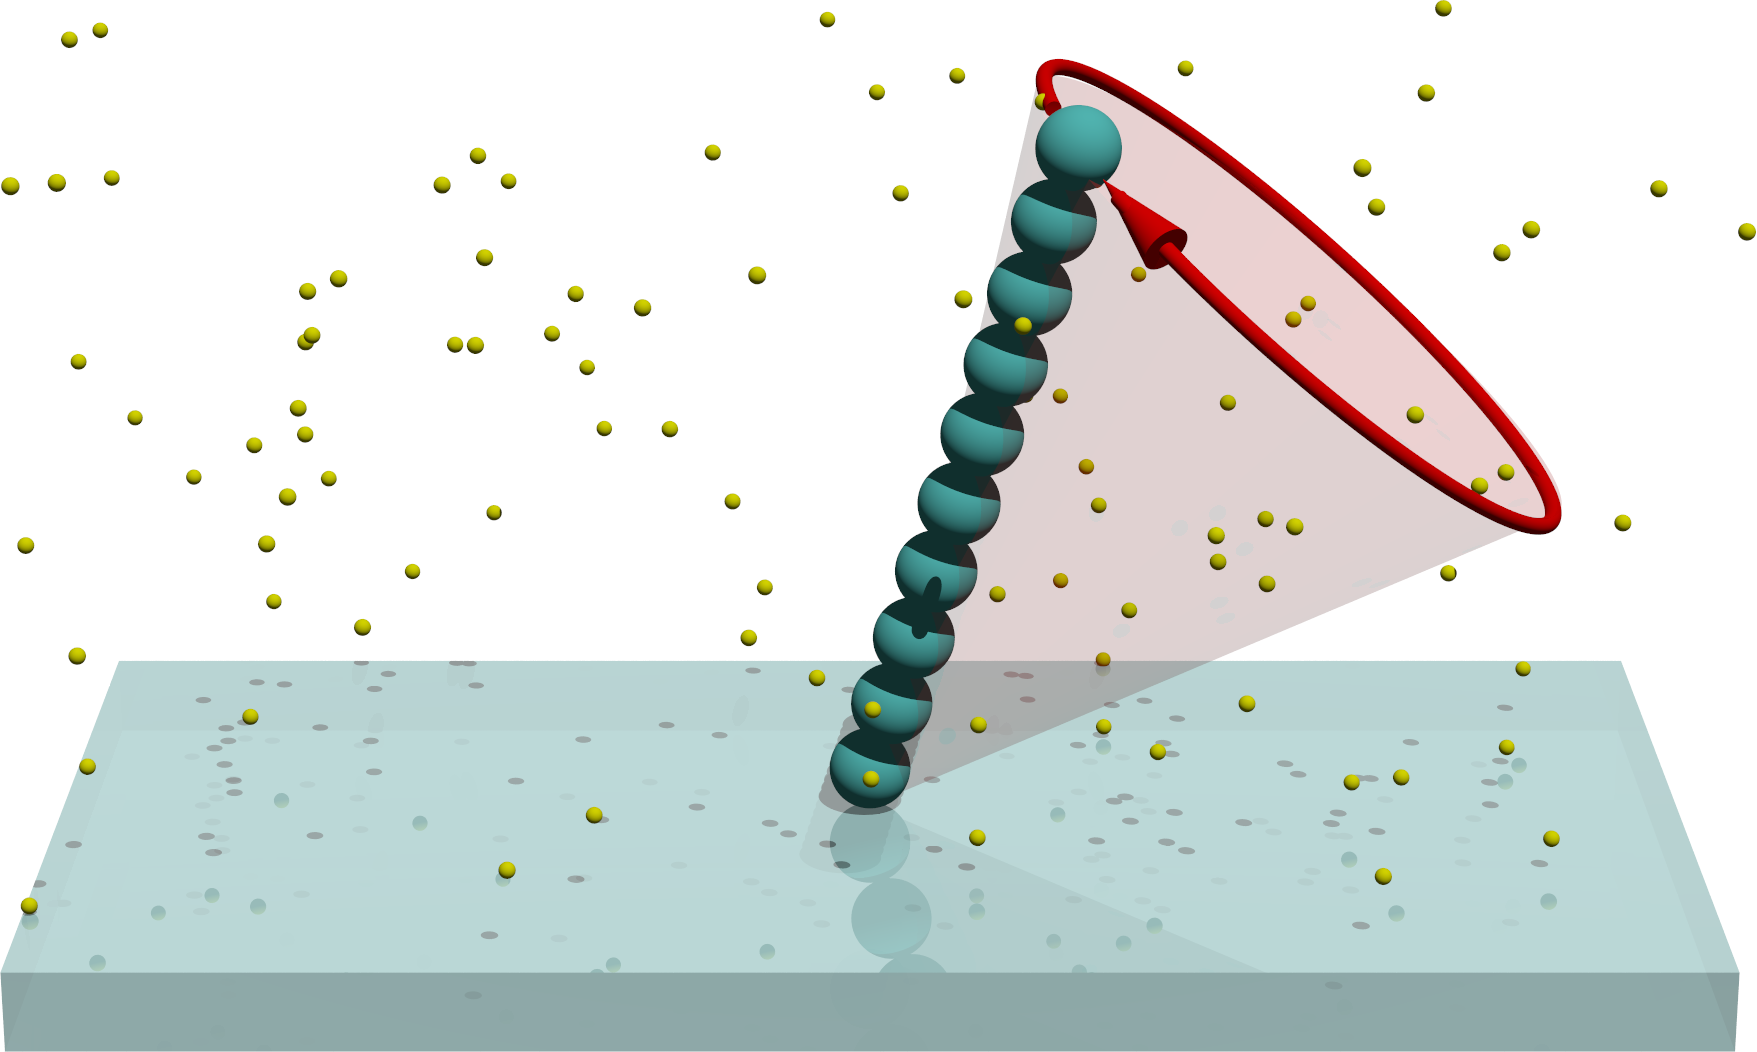
\includegraphics{images_other/absorbing-cilium.png}
    \caption{An illustration of the hydrodynamic simulation. Tracer particles are shown in yellow, and the cilium, simplified to a chain of spheres, is also shown. The trajectory swept out by the cilium is indicated.}
    \label{fig:particle_simulation}
\end{figure}

We then developed a numerical hydrodynamics simulation, wherein individual tracer particles move due to advection and diffusion, and the cilium is approximated by a chain of spheres. The fluid flow due to the motion of these spheres can be computed using superpositions of the Rotne-Prager tensor (Eqs.~(\ref{eq:rp_diag}--\ref{eq:rp_offdiag})), due to the linearity of the Stokes flow. An illustration of the simulation setup is shown in Fig.~\ref{fig:particle_simulation}. 

We used this simulation to understand how much of a gain in chemosensitivity can be achieved by a motile cilium, and found that, provided the cilium beats nonreciprocally in a way that generates a net flow across the cilium, motility can produce a five-fold increase in chemosensitivity compared to a stationary cilium (at realistic cilium Péclet numbers). The increase in chemosensitivity due to cilium motility is even more pronounced than the increase due to cilium geometry, with the chemosensitivity of a motile cilium approaching a factor of $5$ over a stationary cilium at the highest reasonable Péclet numbers a cilium could approach (and hence hugely more sensitive than a chemosensory patch on the cell's surface). At very low Péclet, the cilium barely breaks the diffusion limit, but as the cilium beats faster, the sensitivity rapidly increases. In the high-Péclet regime, the reaction rate scales with $\mathrm{Pe}^{1/3}$, which astoundingly is the same rate that would be found for a sphere in a flow (see box below). The fact that a motile cilium that must pump the fluid itself can reach the same high-Péclet rate scaling as a sphere suspended in a flow is a testament to the efficacy of combining motility with chemosensitivity. This result could go some way to explaining why motile cilia are now known to be chemosensory. The asymmetric beating stroke of the cilium is important, as the net flow it generates is crucial to this increase in chemosensitivity; if a beat is chosen that produces no net flow past the cilium, there is very little increase in chemosensitivity.

\clearpage

\begin{kaobox}[title=Reaction rate for a sphere]
    We can make a scaling argument to derive how the reaction rate $R$ for a sphere in a moving fluid scales with the Péclet number. To begin with, we consider a sphere of radius $a$ in a moving fluid:
    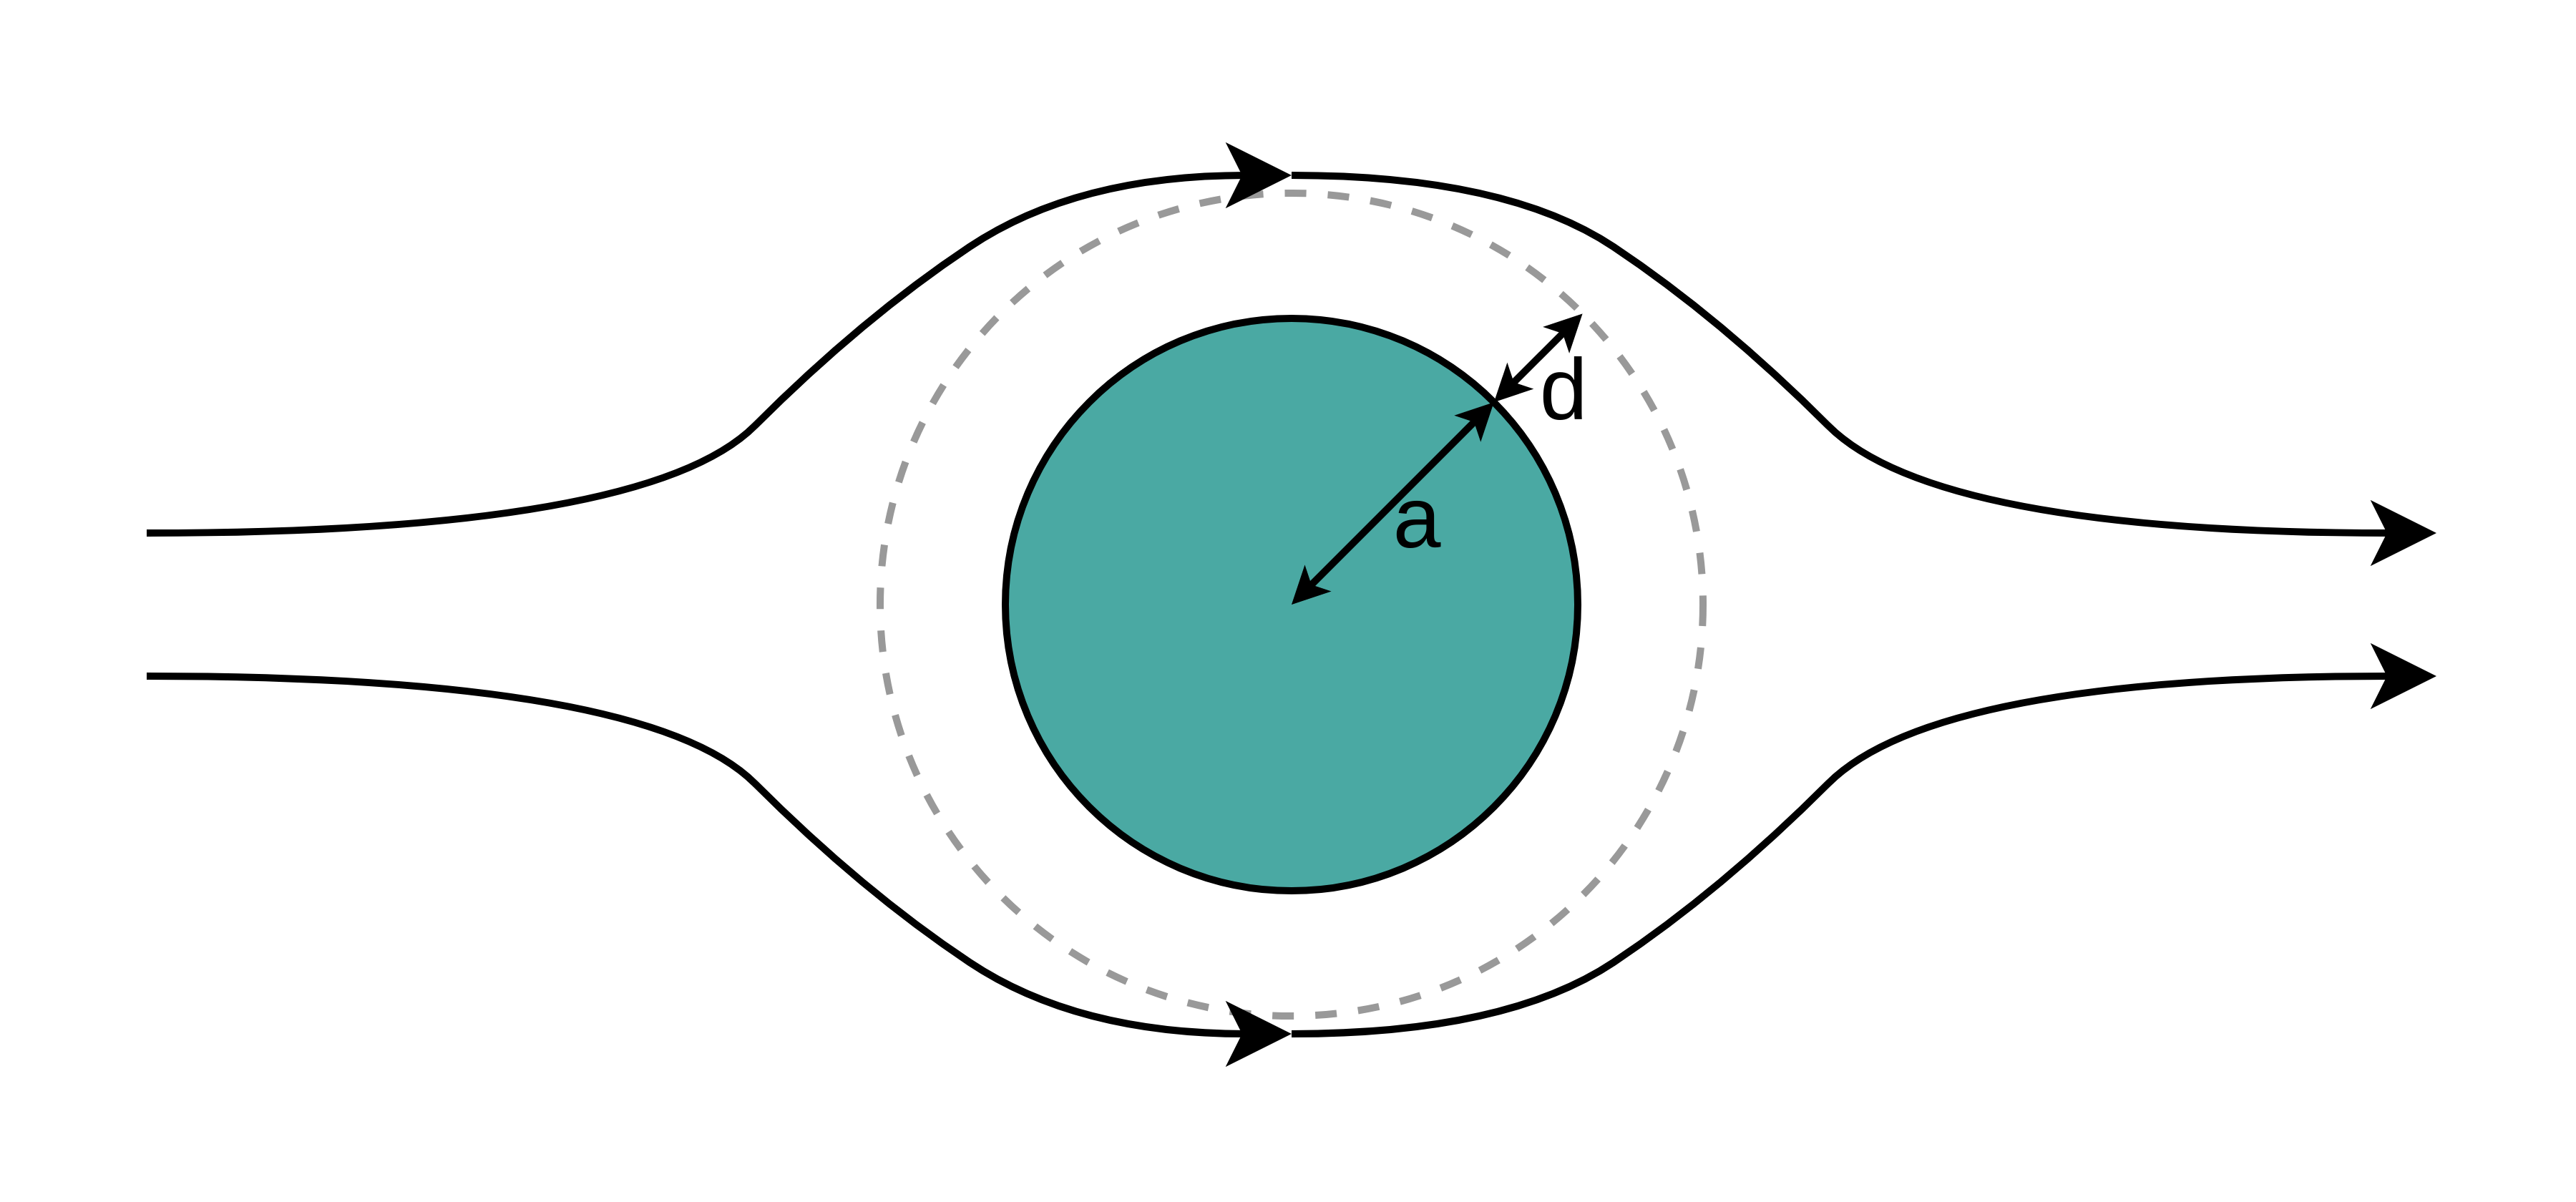
\includegraphics[width=\textwidth]{images_other/sphere_scaling_argument.png}
    We assume that any chemical particles that enter some thin boundary layer of thickness $d$ will make contact with the sphere and be absorbed. Since we know how the diffusion timescale relates to the diffusion length scale (Eq.~\eqref{eq:diffusion_scale}), we know that if the particles take some time $\tau$ to pass the sphere, then
    \begin{equation*}
        d^2 \sim D \tau.
    \end{equation*}
    
    We also know that due to the no-slip condition on the surface of the sphere, the fluid flow very close to the sphere will be well-approximated by a shear flow, and therefore the characteristic flow speed in the boundary layer is $d\dot\gamma$ (where $\dot\gamma$ is the shear rate), which tells us that $\tau \sim 2\pi a/(d\dot\gamma)$.
    
    The reaction rate is then the product of the rate of particle influx ($\sim d\dot\gamma$) with the cross-sectional area of this boundary layer, i.e.
    \begin{equation*}
        R \sim 2\pi a d \cdot d\dot\gamma \sim \left( \frac{a\dot\gamma}{D} \right)^{1/3} = \mathrm{Pe}^{1/3},
    \end{equation*}
    where we have dropped any purely numerical prefactors, as this scaling argument is not nearly precise enough for them to be relevant. Note that we have assumed that $d \ll a$, so that the cross-sectional area of the boundary area can be written as $2\pi ad$; at very high Péclet, this condition is satisfied by definition, so this argument only tells us the scaling behaviour in the high-Péclet limit. Obviously this is an incredibly simplified argument, but much more complicated treatments of the problem give the same result~\cite{bowman_mass_1961}.
    
    It is quite surprising that our results show that a cilium that must pump the fluid itself can reach the same scaling rate as this sphere in a flow, but it is illustrative of just how far motility can increase chemosensitivity.
    
    A similar (albeit more complicated) scaling argument can be made for a cylinder, but due to the Stokes paradox (i.e. there is no well-behaved flow field around a disc in two dimensions at zero Reynolds number) a force density has to be introduced. In this way, a scaling argument can be derived up to a proportionality constant. An approximate value for the proportionality constant had already been found by others~\cite{friedlander_mass_1957}, but we derived an exact value of this constant for the rate per unit length:
    \begin{equation*}
        \frac{dk}{dz} = 3\left(\frac{6}{\pi}\right)^{1/3} \frac{\Gamma(3/4)^{4/3}}{\Gamma(1/3)} D \cdot \mathrm{Pe}^{1/3}.
    \end{equation*}
    The derivation can be found in the appendix of the article below.
\end{kaobox}\nosidecite{bowman_mass_1961, friedlander_mass_1957}

Lastly, we used the same hydrodynamic simulation to investigate the behaviour when placing several chemosensitive motile cilia close together, and found that a bundle motile cilia can be more sensitive together than the same number of individual motile cilia could be apart, i.e. the per-cilium chemosensitivity is higher in a bundle. This result is extremely counter-intuitive, as one would naively expect that many cilia together would all deplete the concentration of signalling molecules and result in a lower per-cilium sensitivity. Instead, every cilium benefits from the fluid flow generated by every other cilium, resulting in the surprising result seen. 



All this shows that by putting chemosensors on cilia, the cell can increase the diffusion limit significantly, and by combining chemosensing with motility, it can break the diffusion limit entirely. This goes some way towards closing some of the open questions introduced in Ch.~\ref{ch:intro}. There are, however, some questions that remain unanswered, which open some possibilities for future work. As previously established, bundles of motile cilia often synchronise, and this work did not examine the impact of metachronal waves on the per-cilium chemosensitivity of a bundle.

There is also potential for a more efficient approach to numerically solving this problem. One consequence of the reciprocal theorem in hydrodynamics is that the particle flux through a surface is invariant under flow reversal, as long as the particle concentration at that surface is uniform~\sidecite{masoud_reciprocal_2019}. If we apply this flow reversal symmetry to the absorption problem, and then apply time-reversal symmetry as well, we have essentially mapped from an absorption problem to an emission problem, where the cilium is now emitting particles but has not changed its trajectory. By inserting and removing particles near the cilium to maintain this concentration, and measuring the flux of particles that escape to infinity, it should be possible to infer the reaction rate. There remain details to be worked out, but it is possible that this approach would increase the efficiency over directly simulating the absorption problem.

% There are some potential applications of this work. For example, very small chemosensors would see an increase in sensitivity if their structure were more cilium-like, or actuated in a way that allows them to move fluid (although progress to date in even making very small chemosensors has been slow~\sidecite{wolfbeis_editorial_2013}, so this application should be considered speculative).

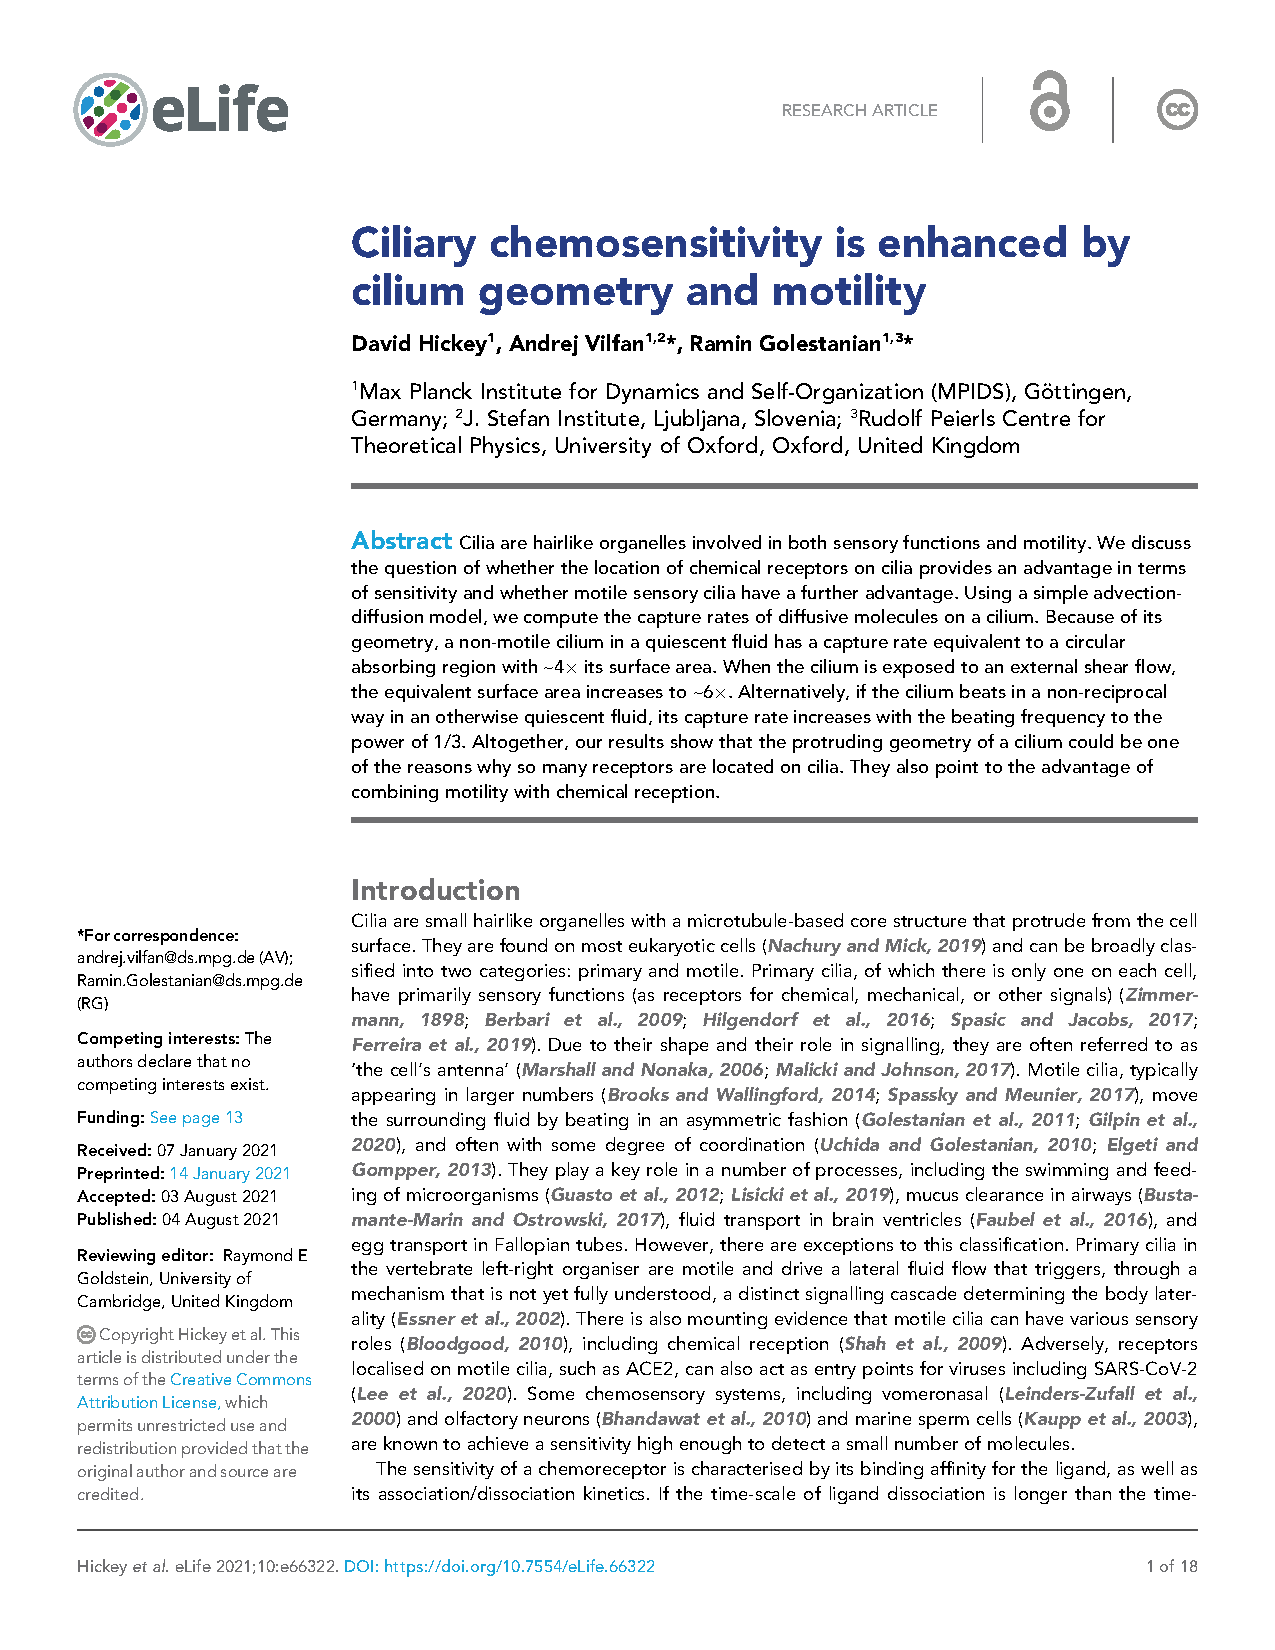
\includepdf[pages=1,pagecommand={ \invisiblesection{Article} \thispagestyle{empty} }]{pdfs/elife-66322-v2.pdf}
\includepdf[pages=2-,pagecommand={ \thispagestyle{empty} }]{pdfs/elife-66322-v2.pdf}

% Now we need a \nocite for every single citation in this paper.
\nocite{nachury_establishing_2019}
\nocite{zimmermann_beitrage_1898, berbari_primary_2009, hilgendorf_primary_2016, spasic_primary_2017, ferreira_cilium_2019}
\nocite{marshall_cilia_2006, malicki_cilium_2017}
\nocite{brooks_multiciliated_2014, spassky_development_2017}
\nocite{golestanian_hydrodynamic_2011, gilpin_multiscale_2020}
\nocite{uchida_generic_2011, elgeti_emergence_2013}
\nocite{guasto_fluid_2012, lisicki_swimming_2019}
\nocite{bustamante-marin_cilia_2017}
\nocite{faubel_cilia-based_2016}
\nocite{essner_conserved_2002}
\nocite{bloodgood_sensory_2010}
\nocite{shah_motile_2009}
\nocite{lee_ace2_2020}
\nocite{leinders-zufall_ultrasensitive_2000}
\nocite{bhandawat_signaling_2010}
\nocite{kaupp_signal_2003}

\nocite{bialek_physical_2005, endres_maximum_2009}
\nocite{berg_physics_1977}
\nocite{adam_reduction_1968}
\nocite{short_flows_2006}

\nocite{marshall_cilia_2006, hilgendorf_primary_2016}
\nocite{marshall_cilia_2006}
\nocite{reiten_motile-cilia-mediated_2017}

\nocite{berg_physics_1977}

\nocite{snow_formulas_1954}

\nocite{challis_olfactory_2015}

\nocite{berg_physics_1977}
\nocite{challis_olfactory_2015, williams_direct_2014}
\nocite{paffuti_results_2018}

\nocite{challis_olfactory_2015}

\nocite{stone_heatmass_1989}

\nocite{bloodgood_sensory_2010}

\nocite{vilfan_generic_2012}

\nocite{smith_fluid_2008}

\nocite{ding_selective_2015, nawroth_motile_2017}

\nocite{berg_physics_1977}

\nocite{frings_single_1990, zhang_ultrasensitive_2013}
\nocite{lai_micro-_2009}

\nocite{ferreira_physical_2017, ferreira_cilium_2019}
\nocite{tanaka_fgf-induced_2005}
\nocite{ding_selective_2015}
\nocite{tripathi_size_2013}
\nocite{nawroth_motile_2017}

\nocite{vilfan_self-assembled_2010, meng_magnetically-actuated_2019, matsunaga_controlling_2019}

\nocite{vilfan_self-assembled_2010}

\nocite{ramirez-piscina_fixed-density_2018}

\nocite{tocino_two-step_2015}

\nocite{berg_physics_1977}

\nocite{masoud_reciprocal_2019}

\nocite{friedlander_mass_1957}
\nocite{vilfan_generic_2012}


\section{Chapter summary}

\begin{itemize}
    \item Chemoreception is an integral part of life, found in all kinds of organisms in all kind of roles, both internal to organisms and externally.
    \item In eukaryotes, a lot of these chemoreceptors are found on cilia. Our work sought to understand some of the reasons why this might be the case.
    \item Our analysis found that all chemoreceptors found on cilia benefit from the geometry of a cilium, which acts to increase their diffusion limit. When a bulk flow is introduced, this geometry-related improvement is even more pronounced.
    \item Motility further increases the chemosensitivity of cilium-bound chemoreceptors. Motile cilia in cilium carpets experience a further increase in per-cilium chemosensitivity over isolated motile cilia, as long as the Péclet number of the beating cilia is high enough.
\end{itemize}

\setchapterpreamble[u]{\optmargintoc}
\chapter{Ciliary synchronisation}
\labch{results_sync}

% 0. Cool hook
Emergent properties, where local rules give rise to widespread global order, are everywhere in biology. The flocking behaviour of birds or sheep can be explained by rules so simple that they can be expressed in a single sentence~\sidecite[75pt]{vicsek_novel_1995, king_selfish-herd_2012} but the resulting motion can look almost impossibly well-coordinated; anyone who has ever seen a thousand-strong flock of starlings knows how complex flocking behaviour can look. But emergent properties are not limited to the scales of entire herds: one very relevant example that can happen even within individual organisms is when motile cilia synchronise with their neighbours to produce globally ordered beating patterns.

% 1. What are metachronal waves? Also I guess I've moved 3 here:
% 3. Where are metachronal waves?
At sufficient density, motile cilia can coordinate their beating with one another, giving rise to collective motion. Sometimes this just means all cilia beating in unison, as in the fallopian tube, where motile cilia beat to move embryos and gametes~\sidecite{lyons_reproductive_2006}. However, one especially interesting coordinated beating mode arises when each cilium beats slightly ahead of its neighbours on one side, but slightly behind its neighbours on the other side. This slight phase difference gives the illusion of a travelling wave, known as a metachronal wave (see Fig.~\ref{fig:metachronal_wave_pov} for an illustration). Metachronal waves are not purely a cilium-related phenomenon: the motion of a millipede's legs~\sidecite[-60pt]{garcia_fundamental_2020}, collective behaviour of worms~\sidecite[-30pt]{peshkov_synchronized_2022}, or the ``Mexican waves'' seen in the stands at sports events are all examples of metachronal waves, though they are less relevant to the work described in this chapter. Ciliary metachronal waves are found in the human trachea, where the waves beat metachronally in order to pump mucus~\sidecite[-100pt]{yaghi_airway_2016, chateau_why_2019}. \textit{Paramecium}~\sidecite[-30pt]{funfak_paramecium_2015} and \textit{Volvox}~\sidecite[0pt]{brumley_hydrodynamic_2012} use metachronally synchronised cilium beating to move fluid around for swimming and feeding. Even shrimp and worms, as well as artificial swimmers like the fantastically named ``krillbot'', have used metachronally synchronised appendages to swim~\sidecite{ford_role_2021, byron_metachronal_2021}. The list of locations where metachronal waves can be found is long, but also surprisingly varied: \textit{Paramecium} is a single multiciliated cell, but \textit{Volvox} is a multicellular colony, and the human trachea is a multicellular part of a larger organism.

\begin{figure}[ht!]
    \centering
    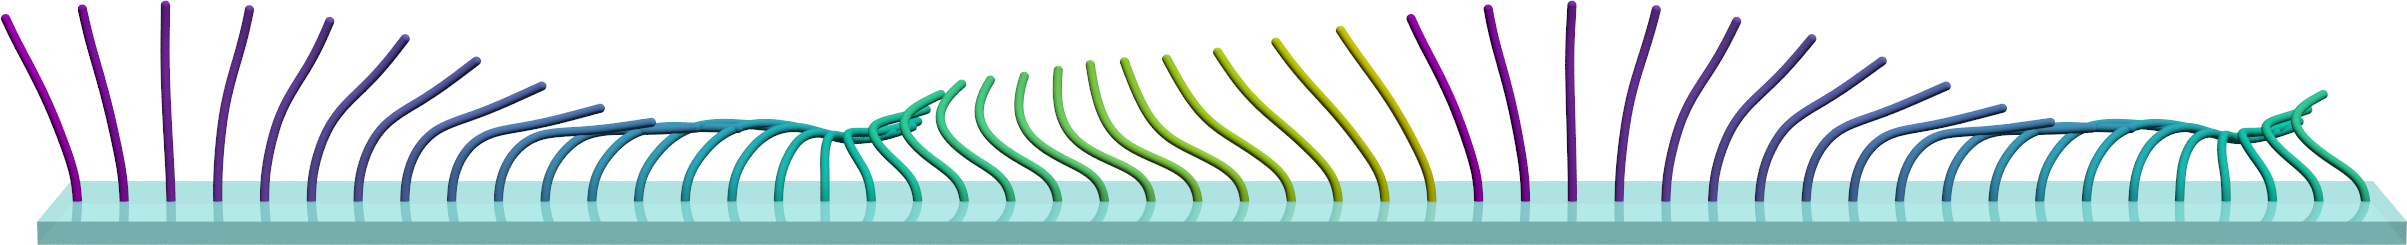
\includegraphics[width=\textwidth]{images_other/enhanced_metachronal1d.png}
    \caption{A metachronal wave in one dimension. Each cilium has a slight phase difference from both of its neighbours. The phase of each cilium is indicated by its colour.}
    \label{fig:metachronal_wave_pov}
\end{figure}

These waves can be categorised into symplectic (meaning that the apparent motion of the wave is in the same direction as the fluid pumping), antiplectic (meaning that the wave direction is opposite the direction of pumping), or if the pumping direction is orthogonal to the wave direction, diaplectic and laeoplectic~\sidecite{zhang_metachronal_2022}.

% 2. Why are metachronal waves?
In cilia, this metachronal coordination is adaptationally advantageous because it increases pumping and swimming speed and energy efficiency~\sidecite{osterman_finding_2011, elgeti_emergence_2013}. One can intuitively see why a metachronal wave might move more fluid than synchronous beating: if a cilium beats in phase with its neighbour, it will experience much lower hydrodynamic drag, and therefore exert lower force on the fluid, hence moving less fluid overall; metachronal waves ensure that no cilium is ever beating exactly in-phase with its neighbour. Under certain circumstances, this gain in efficiency may be much higher for certain types of metachronal waves than others: in the case of pumping of mucus in the human airway, antiplectic waves are more efficient than their symplectic equivalents~\sidecite{chateau_why_2019}. Metachronal waves also reduce energy-wasting collisions between cilia~\sidecite{ringers_novel_2023}, meaning more fluid can be moved with less energy.

% 4. How are metachronal waves? Basal coupling, hydrodynamics, body rocking., peristalsis maybe, etc.
The mechanisms underpinning the emergence of metachronal waves are varied and not completely understood. Cilia on the same cell are connected through coupling between their basal bodies, and it has been shown that in certain cases, basal coupling between cilia on the same cell plays an important role in synchronisation, as hydrodynamically isolated cilia are still capable of synchronising~\sidecite{wan_coordinated_2016, quaranta_hydrodynamics_2015, liu_transitions_2018}. However, in \textit{Volvox}, the cilia are spread across multiple cells in different organisms (which means that basal coupling can be ruled out as a relevant mechanism), and they are still able to synchronise, which suggests that hydrodynamics plays the dominant role under certain circumstances~\sidecite{goldstein_noise_2009}. Steric effects, i.e. direct collisions between cilia, have also been found to play a role~\sidecite{chelakkot_synchronized_2021}. Although small numbers of bacterial flagella can synchronise due to the rocking of the bacterium they are all attached to~\sidecite{geyer_cell-body_2013}, this probably doesn't bear much relevance to metachronal waves in cilia, where there are often hundreds or thousands of cilia beating together.

\section{Models of synchronisation}

The literature contains many models that seek to explain ciliary synchronisation. Though some models account for things like body-rocking~\cite{geyer_cell-body_2013} or basal coupling~\sidecite{liu_transitions_2018, guo_intracellular_2021, klindt_-phase_2017}, in this section we will focus on models of hydrodynamic coupling, as they are more relevant to our work.

One of the simplest models of synchronising oscillators is the Kuramoto model, wherein the oscillators have some (not necessarily identical) intrinsic frequencies $\omega_i$ and are globally coupled to one another by a function that depends upon their phase difference~\sidecite{pikovskij_synchronization_2007}:
\begin{equation}
    \dot{\phi_i} = \omega_i + \frac{\epsilon}{N} \sum_{j=1}^N H(\phi_i - \phi_j).
\end{equation}
This model is very simple, and in the large-$N$ limit, the dynamics can be solved exactly. However, most models of hydrodynamic synchronisation are slightly more complicated than this globally-coupled Kuramoto model, because hydrodynamic interactions are dependent on distance, and the coupling strength is not always purely a function of the phase difference.

Some approaches model the cilia as long filaments with active driving forces~\sidecite{man_multisynchrony_2020, goldstein_elastohydrodynamic_2016, guirao_spontaneous_2007, gueron_energetic_1999, kim_pumping_2006}. Others consider a very detailed treatment of the cilium: \etalcite{solovev_lagrangian_2021}, for example, have developed an approach to simulation of cilia that works for arbitrary cilium shapes and trajectories, though this results in sufficient complexity that a lot of variables must be precomputed in order to be able to solve the equations of cilium motion in reasonable time.

The approach favoured by many, including us, is to model the cilium as a sphere on a fixed trajectory but with a variable speed~\sidecite{vilfan_hydrodynamic_2006, meng_conditions_2021, niedermayer_synchronization_2008, uchida_generic_2011, uchida_hydrodynamic_2012, nasouri_hydrodynamic_2016, kanale_spontaneous_2022, wollin_metachronal_2011, uchida_synchronization_2010}. There are a number of advantages to this: the hydrodynamic force on a sphere in the presence of a boundary can be computed using the Rotne-Prager mobility tensor (Eqs.~(\ref{eq:rp_diag}--\ref{eq:rp_offdiag})) in an efficient manner, and by making simple adjustments to the trajectory, it is possible to recreate the power/recovery stroke behaviour seen in most biological motile cilia.

No matter the approach taken, it must be remembered that the Stokes flow is time-reversible, but synchronisation is by definition an irreversible process. The model must therefore find some way to break this symmetry. Possibilities that have seen success in the literature include additional degrees of freedom per cilium (which can automatically be achieved by modelling the cilia as flexible filaments that can bend in various directions), asymmetric spatial arrangements of cilia~\cite{vilfan_hydrodynamic_2006}, driving forces or trajectories that break the right symmetries~\cite{fruchart_non-reciprocal_2021, kanale_spontaneous_2022}\nosidecite{fruchart_non-reciprocal_2021}, or (for example) nonlinear driving mechanisms that change the driving direction once a certain position is reached~\sidecite{elgeti_emergence_2013}.

Most models of synchronisation make two additional simplifications: firstly, it is common for near-field hydrodynamic interactions to be neglected~\cite{meng_conditions_2021, niedermayer_synchronization_2008}. This is an attractive simulation in many cases because it massively simplifies the computational effort required, as the far-field terms that remain in the limit of large intercilium separation are much simpler to compute than the near-field terms, and can even be treated analytically~\cite{niedermayer_synchronization_2008}. Secondly, many modelling approaches have required the system to have periodic boundary conditions~\cite{niedermayer_synchronization_2008, meng_conditions_2021, wollin_metachronal_2011, uchida_synchronization_2010}, as without these, the cilia near the edges have a lower number of neighbours, which can affect their beating frequency and lead to the breaking up of order~\cite{kavre_hydrodynamic_2015, hamilton_chimera_2017, niedermayer_synchronization_2008}\nosidecite{kavre_hydrodynamic_2015, hamilton_chimera_2017}.

However, these simplifications are often biologically implausible. For example, intercilium spacing in many biological systems is much less than the cilium length~\sidecite{bouhouche_paramecium_2022, sleigh_propulsion_1988}, which is at odds with assumption of a far-field limit. While there do exist periodic one-dimensional arrays of cilia, such as in starfish larvae~\sidecite{strathmann_feeding_1971} or the oral cilia of \textit{Stentor}~\sidecite{wan_reorganization_2020}, they are far from the norm. We will later show that both of these simplifications are inadequate when considering nonreciprocal hydrodynamic coupling of cilia.

% 1. Broad modelling approaches used. Start with Kuramoto and Kuramoto-style models. Filaments (Multisynchrony in..., Gueron&Levit-Gurevich 1999, Guo&et.al 2018), spheres-on-a-stick (Fanlong, Babak&Elfring, Vilfan&Jülicher 2006, Wollin&Stark2011 [though they used point particles], Kanale), extended multiscale treatments (Solovev&Friedrich×several). Bring up some hydrodynamic models that assume far-field limit. Discuss the extent to which models rely on PBCs.

% Talk about symmetry breaking. Multiple DoF, weird arrangements, nonuniform driving forces/trajectories, or nonlinear driving mechanisms.

\section{Nonreciprocity in active systems}
% Do we need a section on background physics? I think the definition of nonreciprocal is pretty important.
% In active systems...
In active systems, the influence exerted by one body on another need not be reciprocal~\sidecite{fruchart_non-reciprocal_2021}. For example, under certain circumstances, the motion of an enzyme can be affected by a chemical gradient, which is itself affected by another enzyme. In this way, one enzyme exerts an influence on another, but the reverse is not true~\sidecite{agudo-canalejo_active_2019}. Similar effects can be observed in flocking behaviour~\sidecite{nagy_hierarchical_2010}, systems of neurons~\sidecite{montbrio_kuramoto_2018}, artificial active particles~\sidecite{lavergne_group_2019}, and countless others.

This nonreciprocal coupling can also happen in systems of hydrodynamic interactions. The Lorentz reciprocal theorem can be expressed in its integral form as
\begin{equation}
    \iint_S \mathbf{u} \cdot (\mathbf{\sigma}' \cdot \hat{\mathbf{n}}) \, \mathrm{d}S = \iint_S \mathbf{u}' \cdot (\mathbf{\sigma} \cdot \hat{\mathbf{n}}) \, \mathrm{d}S,
\end{equation}
where $S$ is the surface of a body, $\mathbf\sigma$ is the hydrodynamic stress on the body's surface, and $\hat{\mathbf{n}}$ is the normal to the body's surface~\sidecite{masoud_reciprocal_2019}. 
This is an incredibly important result in hydrodynamics, as it means that, depending on the velocities of the two bodies, the force on each body can have the same or different signs. This differs from Newton's third law, under which the forces would always have the opposite sign, and is a consequence of hydrodynamic interactions being dissipative rather than conservative. This opens up a lot of possibilities for nonreciprocal coupling in hydrodynamics, where if two identical hydrodynamically coupled particles have very different velocities, they can experience differing forces (and vice versa: two bodies with very different active driving forces can induce differing velocities), which can be an extremely potent effect in inducing synchronisation. Some models of hydrodynamic rotor synchronisation have already included nonreciprocal hydrodynamic coupling~\sidecite{uchida_synchronization_2010} (though it should be stressed that these rotors are quite unlike cilia). % Andrej doesn't think this is a fair summary of this work. Maybe because it makes it sound too similar to ours when it's very different?

In the context of cilia, this means that one cilium can influence its neighbour more than vice versa. Factors such as the driving force that the cilium exerts and the nonuniformity of internal and external drag coefficients over the cilium trajectory can all make the cilium more susceptible to being perturbed by a neighbour in certain parts of its trajectory than in others. This combined with the varying velocity of the cilium relative to its neighbours can give rise to a very asymmetric interaction strength. Indeed, other work has found that asymmetric coupling can be relevant for ciliary synchronisation, such as \etalcite{niedermayer_synchronization_2008}. However, the model used by \citeauthor*{niedermayer_synchronization_2008}~\cite{niedermayer_synchronization_2008} did not consider near-field hydrodynamics, rather solving in the far-field limit, and found that cilia with the same intrinsic beating frequency could only synchronise to a state with identical phases, i.e. they did not find the phase lag characteristic of metachronal waves. Our model of ciliary synchronisation, explained in the following section, relies heavily on nonreciprocal hydrodynamic coupling to synchronise.

% The idea of nonreciprocity enabling oscillators to synchronise is not completely new. Even non-active pendulums can create localised structures such as travelling waves when nonreciprocally coupled to one another, and disturbances in one part of the chain will tend to favour travelling in one direction over another \sidecite{pinto-ramos_nonreciprocal_2021}.

\section{Our work}
% 5. What we done, with emphasis on nonreciprocity
In this work, we developed a simple model of ciliary synchronisation. The cilium is represented as a spherical bead on a titled circular trajectory, which despite its simplicity, still has separate power and recovery strokes. The tilting of the trajectory breaks time-reversal symmetry, meaning that the beat avoids the problem posed by scallop theorem, and is therefore able to generate a net fluid flow.
% Each cilium has a driving force and internal friction coefficient which are purely functions of its phase angle. While the cilia are all confined to their circular trajectories, hydrodynamic interactions between cilia cause some cilia to move faster or slower than others along their trajectories, eventually leading from a random initial state to a metachronally synchronised final state. Some examples of possible simulated lattices are shown in Fig.~\ref{fig:sync_sim}.

\begin{figure*}
    \begin{subfigure}[t]{0.49\linewidth}
        \centering
        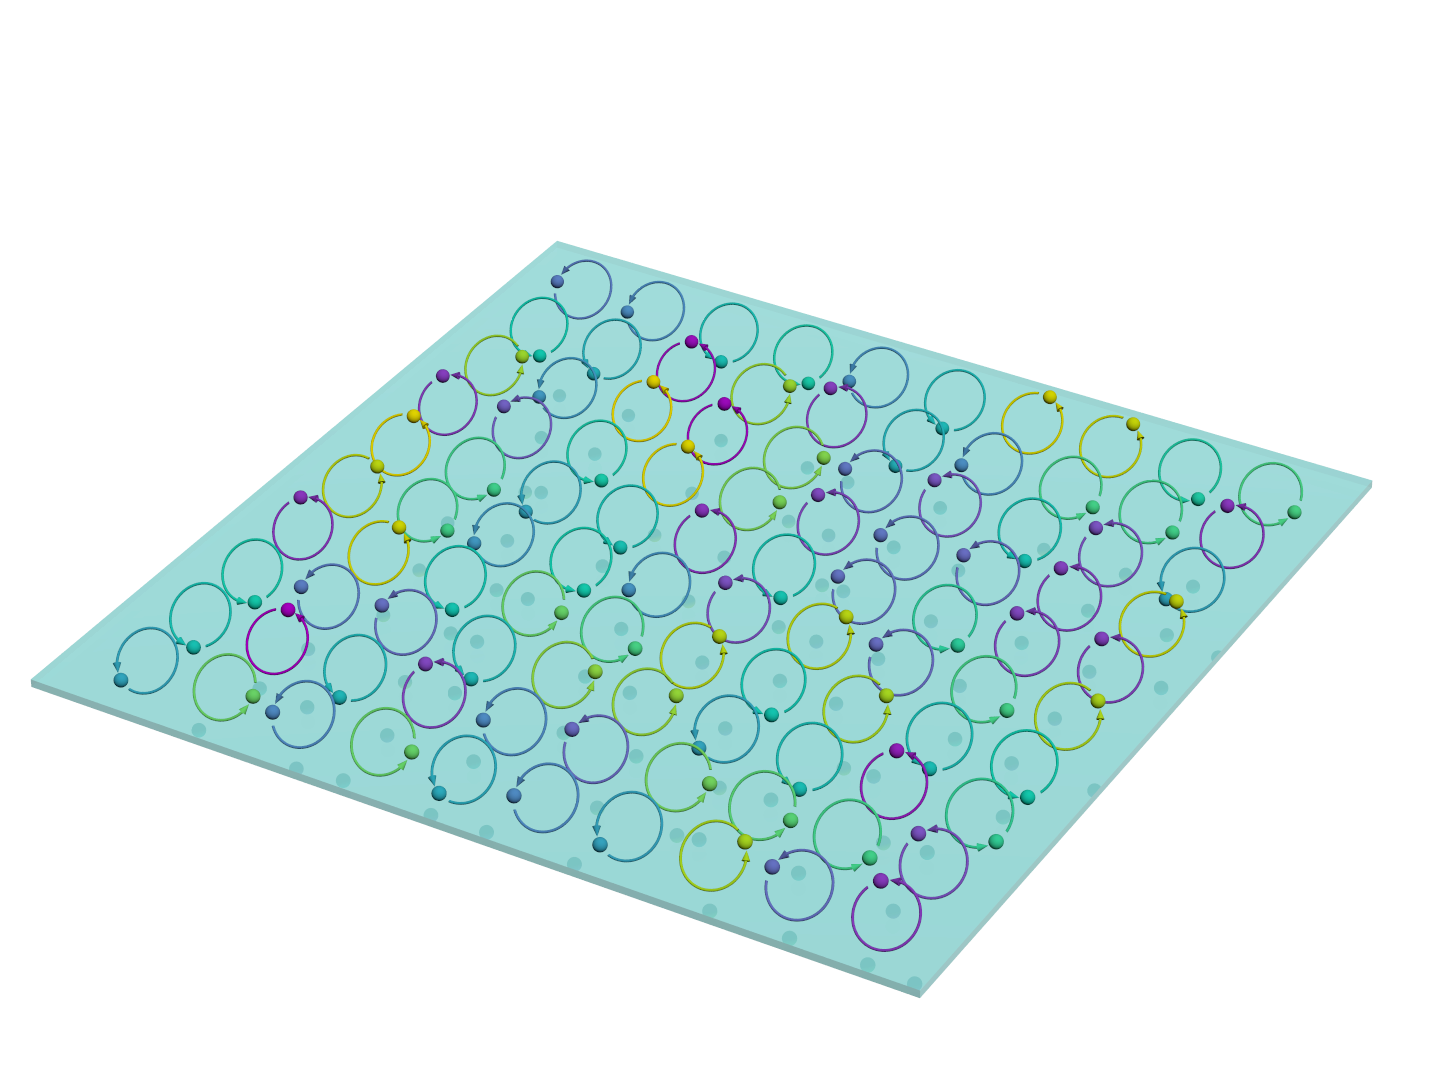
\includegraphics[width=1\textwidth]{images_other/enhanced_2d_unsync.png}
        \caption{Unsynchronised state}
    \end{subfigure}
    ~
    \begin{subfigure}[t]{0.49\linewidth}
        \centering
        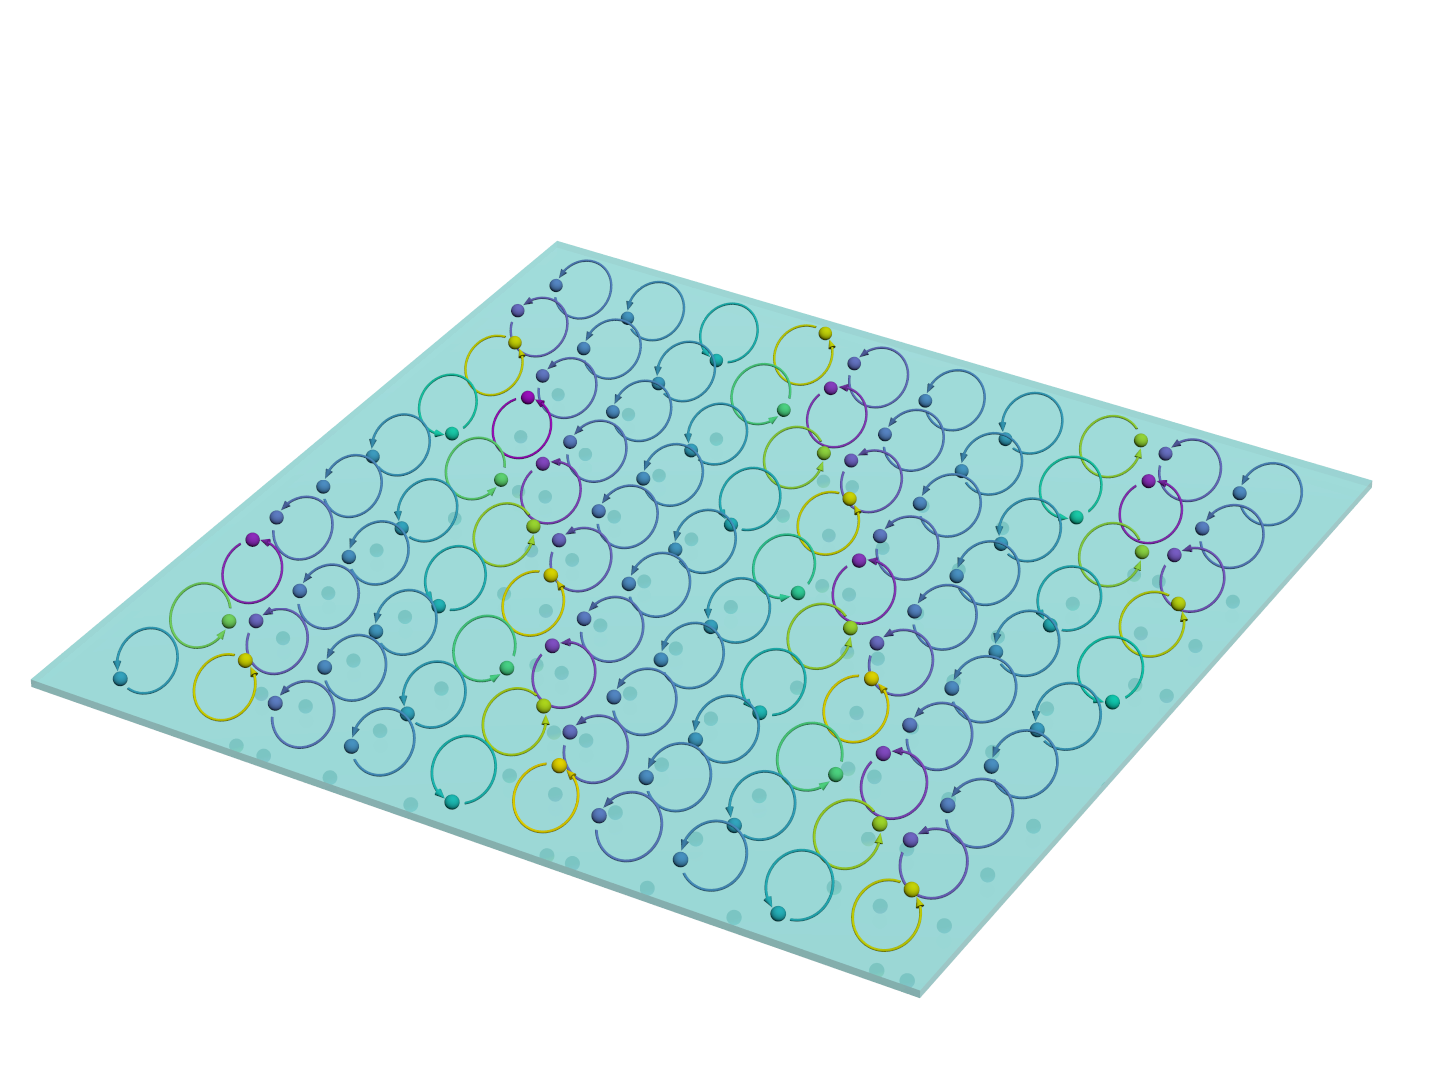
\includegraphics[width=1\textwidth]{images_other/enhanced_2d_sync.png}
        \caption{Metachronally synchronised state}
    \end{subfigure}
       
    \caption{Potential states of the simulation, showing the phase and position of each cilium. Each cilium has an identical intrinsic frequency. Each cilium is confined to a tilted circular trajectory, where the tilt ensures that the cilia have a power and recovery stroke despite the model's simplicity. Each cilium has a driving force and friction coefficient that is a function of its phase. Hydrodynamic interactions between cilia cause some cilia to move around their trajectory slightly faster than others, eventually leading from an unsynchronised initial state (as in (a)) to a stable synchronised state (as in (b)).}
    \label{fig:sync_sim}
\end{figure*}

The cilium has a phase-dependent driving force $\mathbf{F}^\text{dr}(\phi)$ and internal friction coefficient $\Gamma(\phi)$, which were tuned to give sensible cilium motion. We considered a system of many such model cilia on various lattices, where the cilia could interact with one another hydrodynamically. The governing equation for each cilium may be written as
\begin{equation}
    0 = \mathbf{F}^\text{dr}(\phi_i) + \mathbf{F}^\text{c}(\phi_i) - \Gamma(\phi_i)\mathbf{v}_i - \sum_j \mathbf{\Gamma}_{ij} \mathbf{v}_j,
\end{equation}
where $\mathbf{F}^\text{c}$ are the forces that constrain the cilium to its circular trajectory, and are by definition always perpendicular to the trajectory, so that they don't change its speed along the trajectory. $\Gamma_{ij}$ is the friction tensor, which gives the force response at cilium $i$ due to a velocity at $j$ -- essentially, the opposite of the mobility tensor. Each cilium moves around its trajectory with some intrinsic frequency, but the motion of other cilia perturbs the fluid which in turn perturbs the cilia, causing cilia to move along their trajectory with varying speeds.

The entire system was solved numerically to find the time-evolution of the system, starting from a random initial state. We found that under normal circumstances with an open boundary, the system of cilia can quickly synchronise to a deterministic metachronal state, with a relaxation time that scales linearly with the system time -- a good improvement over many other models of this same phenomenon. However, when near-field hydrodynamic effects are suppressed, the synchronisation time increases dramatically, and this linear dependence is lost; this is because of the nonreciprocal coupling that is now suppressed. Additionally, the final synchronised state can now consist of multiple wavevectors, which depends entirely on the random initial configuration. When introducing periodic boundary conditions, we found that the nonreciprocity was now counterproductive, as patches of disorder could now spread in the same way as patches of order, without being extinguished.

These results have huge implications for the importance of nonreciprocal coupling in ciliary synchronisation. Near-field effects, whereby a combination of cilium position, driving force, and hydrodynamic and internal condition make the coupling nonreciprocal, mean that a cilium can entrain its neighbour but not vice versa. This allows the order to spread extremely quickly through the system, starting from one edge and spreading linearly, and means that order is robust even at open boundaries. Without these nonreciprocal near-field effects, ciliary synchronisation takes an order of magnitude longer. The final state would no longer be deterministic, and since antiplectic and symplectic waves pump with different speeds and efficiencies, this could have an impact on the pumping or swimming efficiency.

Secondly, these results show that hydrodynamics is sufficient for swift synchronisation in at least some circumstances, so basal coupling is not an absolute requirement for synchronisation. In real cilia, the intercilium distances can be much lower than what we have simulated, so it is possible that the hydrodynamic interactions, especially the near-field interactions, are even more relevant and can explain the extremely rapid synchronisation seen in ciliates.

% 6. Why we done it
This work shows that hydrodynamic interactions, in particular nonreciprocal near-field interactions, are sufficient to induce and maintain stable order in finite systems. This represents a step forward in our understanding of the emergence of metachronal waves, as most models have hitherto been unable to support stable order in finite systems, and have been forced to rely on periodic boundary conditions in order to prevent boundary effects from disrupting the order of the system. The ability to produce stable metachronal waves in finite systems is highly desirable, as open boundaries are common in experimental systems, whereas there are only a few cases where one can find unbroken lines of cilia that approximate periodic boundaries.

% \invisiblesection{Article}
\includepdf[pages=1,pagecommand={ \invisiblesection{Article} \thispagestyle{empty} }]{pdfs/Nonreciprocal_interactions____without_branding-1.pdf}
\includepdf[pages=2-,pagecommand={ \thispagestyle{empty} }]{pdfs/Nonreciprocal_interactions____without_branding-1.pdf}

% Now we need a \nocite for every single citation in this paper.
\nocite{brennen_fluid_1977}
\nocite{nachury_establishing_2019}
\nocite{faubel_cilia-based_2016}
\nocite{yaghi_airway_2016}
\nocite{bhandawat_signaling_2010}
\nocite{dasgupta_cilia_2016}
\nocite{prandtl_1926_aufgaben}
\nocite{taylor_1951_analysis}
\nocite{golestanian_hydrodynamic_2011}
\nocite{osterman_finding_2011, elgeti_emergence_2013}
\nocite{ringers_novel_2023}
\nocite{hickey_ciliary_2021}
\nocite{funfak_paramecium_2015}
\nocite{funfak_paramecium_2015}
\nocite{osterman_finding_2011}
\nocite{brumley_hydrodynamic_2012}
\nocite{yaghi_airway_2016}
\nocite{chateau_why_2019}
\nocite{byron_metachronal_2021}
\nocite{knight-jones_relations_1954}
\nocite{goldstein_noise_2009}
\nocite{wan_coordinated_2016, quaranta_hydrodynamics_2015, liu_transitions_2018}
\nocite{narematsu_ciliary_2015}
\nocite{golestanian_hydrodynamic_2011}
\nocite{reichert_2005_synchronization,guirao_spontaneous_2007,niedermayer_synchronization_2008,qian_minimal_2009,uchida_hydrodynamic_2012,man_multisynchrony_2020}
\nocite{vilfan_hydrodynamic_2006}
\nocite{uchida_synchronization_2010,uchida_synchronization_2010-1,saha_pairing_2019, meng_conditions_2021, kanale_spontaneous_2022, uchida_generic_2011, uchida_hydrodynamic_2012,maestro_control_2018}
\nocite{wollin_metachronal_2011,elgeti_emergence_2013, guo_bistability_2018, chakrabarti_hydrodynamic_2019, chakrabarti_multiscale_2022}
\nocite{masoud_reciprocal_2019}
\nocite{niedermayer_synchronization_2008}
\nocite{soto_2014_self-assembly,soto_2015_self-assembly,agudo-canalejo_active_2019,saha_pairing_2019, saha_scalar_2020, loos_irreversibility_2020, fruchart_non-reciprocal_2021, osat_non-reciprocal_2023}
\nocite{uchida_synchronization_2010}
\nocite{solovev_synchronization_2022}
\nocite{solovev_synchronization_2022}
\nocite{kavre_hydrodynamic_2015}
\nocite{hamilton_chimera_2017}
\nocite{meng_conditions_2021, elgeti_emergence_2013, uchida_synchronization_2010, uchida_synchronization_2010-1, niedermayer_synchronization_2008, nasouri_hydrodynamic_2016, solovev_synchronization_2022, mannan_minimal_2020, wollin_metachronal_2011}
\nocite{wan_reorganization_2020}
\nocite{strathmann_feeding_1971}
\nocite{brennen_fluid_1977}
\nocite{vilfan_generic_2012}
\nocite{meng_conditions_2021}
\nocite{uchida_generic_2011, uchida_hydrodynamic_2012,kanale_spontaneous_2022}
\nocite{vilfan_hydrodynamic_2006}
\nocite{vilfan_hydrodynamic_2006}
\nocite{elfring_2009_hydrodynamic,golestanian_hydrodynamic_2011}
\nocite{meng_conditions_2021}
\nocite{vilfan_hydrodynamic_2006,elfring_2009_hydrodynamic,golestanian_hydrodynamic_2011,solovev_lagrangian_2021,solovev_synchronization_2022-1}
\nocite{boselli_fluid_2021}
\nocite{meng_conditions_2021, elgeti_emergence_2013, uchida_synchronization_2010, uchida_synchronization_2010-1, niedermayer_synchronization_2008, nasouri_hydrodynamic_2016, solovev_synchronization_2022, mannan_minimal_2020, wollin_metachronal_2011, aref_fluid_2021, ringers_novel_2023}
\nocite{wollin_metachronal_2011}
\nocite{osterman_finding_2011, elgeti_emergence_2013}
\nocite{kanale_spontaneous_2022}
\nocite{meng_conditions_2021}
\nocite{bouhouche_paramecium_2022}
\nocite{sleigh_propulsion_1988}
\nocite{brumley_hydrodynamic_2012}
\nocite{boselli_fluid_2021}
\nocite{solovev_synchronization_2022}
\nocite{kavre_hydrodynamic_2015}
\nocite{chelakkot_synchronized_2021}
\nocite{liu_transitions_2018}
\nocite{brumley_flagellar_2014}
\nocite{soh_intracellular_2022}
\nocite{theers_synchronization_2013,wei_measurements_2021}
\nocite{gilpin_multiscale_2020}
\nocite{solovev_synchronization_2022-1}
\nocite{bottier_how_2019}
\nocite{verra_ciliary_2013}
\nocite{horani_advances_2018}
\nocite{nawroth_stem_2019}
\nocite{toonder_microfluidic_2013}
\nocite{blake_note_1971}
\nocite{vilfan_self-assembled_2010}
\nocite{young_iterative_1971}
\nocite{welch_use_1967}

\section{Chapter summary}

\begin{itemize}
    \item Metachronal waves are relatively common phenomena that lead to increased pumping effectiveness in cilia.
    \item Even in finite systems, hydrodynamic interactions are sufficient to give fast stable metachronal waves.
    \item Nonreciprocity of hydrodynamic interactions is crucial to retain this fast synchronisation. If the nonreciprocity is somehow suppressed, synchronisation is now much slower and the final synchronised state is no longer deterministic, which (given that research has shown that antiplectic waves are more efficient than symplectic ones~\sidecite{chateau_why_2019}) could lead to decreased pumping efficiency even in the steady-state.
\end{itemize}
\setchapterpreamble[u]{\optmargintoc}
\chapter{Conclusion}
\labch{conclusion}

\begin{quote}
    \textit{%
        Treacle nodded. ``I hadn't looked at it like that,'' he said, ``but you're absolutely right. He's really pushed back the boundaries of ignorance. There's so much about the universe we don't know.''%
    }%
    % \textit{Science is not about building a body of known ‘facts’. It is a method for asking awkward questions and subjecting them to a reality-check, thus avoiding the human tendency to believe whatever makes us feel good.}
    
    \hfill Sir Terry Pratchett,~\textit{Equal Rites}
\end{quote}

% Good hook
Given the ubiquity of cilia, and their centrality to so many biological processes, it is partly a shame, but mostly a fantastic opportunity, that we still don't fully understand why they are built the way they are and act the way they do, and they continue to be the source of so many interesting open questions. We have tried to make some progress towards closing some of these open questions, and in the process we have opened a few new ones -- as Pratchett put it, in this work we have pushed the boundaries of ignorance, continuing a process that presumably began when the first organism with eyes looked up at the stars and wondered what they were.

% My cunning plan:
% 1. What have we learned? What are the implications?
% 2. What're the limitations, or things we get wrong?
% 3. Future work, applications, and galaxy-brain ideas

% ========================== %
% === 1. WHAT WE LEARNED === %
% ========================== %
% This bit could be much longer. Komal said more. Mirna/Lorenzo said about the same amount per chapter, but had more chapters.
In Chapter~\ref{ch:results_particle}, by considering the mass transport to a perfectly reactive cilium, we found that the geometry of the cilium confers a chemosensory advantage over a chemosensory patch, and that motility confers a chemosensory advantage over immotility, even when motile cilia are bunched together in groups. These results were robust at a wide range of biologically plausible values of the cilium beating frequency, and would go some way towards explaining why chemoreceptors are often found on cilia (both motile and primary). 

That said, the model considered in this chapter has some limitations. We assumed that particles are absorbed by the cilium immediately upon first touching it, which is only justified if the receptors cover a sufficient fraction of the surface area (though the required fraction is extremely low: in the absence of advection, only 1\% of the surface must be covered by receptors to achieve near-perfect sensitivity~\sidecite{berg_physics_1977}). The Rotne-Prager mobility tensor that we used does not perfectly satisfy the no-slip boundary, especially at high Péclet numbers, which should not change the qualitative story told by the results but could have a quantitative impact. We have also assumed that the signalling molecules being detected are extremely small relative to the cilium, which may not be completely true for large protein complexes or vesicles.

Then, in Chapter~\ref{ch:results_sync}, we considered the interactions of a lattice of cilia, and found that stable order could emerge in linear time even in finite systems with open boundaries, provided the hydrodynamic intercilium coupling was nonreciprocal. Without this nonreciprocal coupling, the order emerged in nonlinear time, and the final state was non-deterministic. This suggests that for cilia, nonreciprocal coupling is incredibly important.

Possibly the primary limitation in the model in this chapter is that it does not consider the role of non-identical cilium forms and noisy behaviour. Thermal noise will play a role in cilium motion simply due to their small size, but additionally the driving process for the motile cilium is itself stochastic, i.e. there are active fluctuations~\sidecite{ma_active_2014}. In biological systems, ciliary synchronisation is highly resistant to noise~\sidecite{gilpin_multiscale_2020} and it would be useful to know if this behaviour is reproduced by our model. Different cilia, even on the same cell, can have differing intrinsic beat frequencies~\sidecite{goldstein_noise_2009}, and there is no reason we would necessarily expect every cilium to be identical in length, especially when they have been subject to damage or disease~\sidecite{leopold_smoking_2009}. The simplification of the entire cilium to a single sphere on a circular trajectory simplified the calculations and simulation to a huge degree, and probably does not qualitatively affect the results, but it does remove certain near-field effects. Given that we found near-field hydrodynamic interactions to be incredibly important to synchronisation, it is possible that the synchronisation would be even faster with a cilium model more akin to the chain of beads used in Ch.~\ref{ch:results_particle}, so this is another avenue worth exploring.

Considering the work as a whole, we see that interactions between motile cilia are extremely beneficial, increasing sensing and pumping efficiency. It should therefore come as no surprise that motile cilia are often found in carpets, as the close proximity ensures that per-cilium chemosensitivity sees an improvement, as well as permitting the cilia to benefit from near-field hydrodynamic interactions so that they can coordinate their beating.


% ======================================= %
% === 3. FUTURE WORK AND APPLICATIONS === %
% ======================================= %
Other than addressing the limitations discussed above, there is plenty of additional research to be done on these and similar models. For example, we showed that motile cilia in close proximity can quickly synchronise to form a metachronal wave, and we also showed that a bundle of motile cilia with random phases can be more chemosensitive per cilium than a single motile cilium on its own. It would be interesting to see whether this increase is retained if the cilium phases are metachronally synchronised rather than randomised, which seems probable given that the high volume flow rates achieved by metachronal waves could draw a large amount of signalling molecules into the cilium carpet.

Coronaviruses in general frequently attack and damage ciliated cells~\sidecite{jonsdottir_coronaviruses_2016}, and patients with SARS-CoV-2 are known to have ciliated cells that have lost their cilia entirely~\sidecite{buqaileh_can_2021}, resulting in a reduced rate of mucus clearance from the lungs and airway by cilia~\sidecite{robinot_sars-cov-2_2021}. Since this mucociliary clearance is one of the first lines of defence against airborne pathogens and particulates, this results in higher susceptibility to disease and damage~\sidecite{tilley_cilia_2015}. It is possible that the lower cilium density results in a loss of metachronal coordination, which in turn causes this decreased pumping efficiency seen in SARS-CoV-2 patients, but it could simply be the case that a lower cilium density results in impeded clearance of mucus from the airways due to fewer cilia moving mucus. Better understanding the mechanisms underlying this reduced pumping efficiency could be of significant value, and could be achieved by using a version of our model to investigate how the loss or damage of cilia affects the ability of ciliary carpets to synchronise, though it would need to be adapted to account for the non-Newtonian nature of the mucus.

% In swimmers like \textit{Paramecium}, some of the cilia are found in doublets~\sidecite{bouhouche_paramecium_2022}, where two cilia are displaced by a distance much smaller than the typical intercilium distance. It's not clear whether this carries some sort of advantage in swimming efficiency, swimming speed, or cilium synchronisation, but with our model of cilium synchronisation, we could potentially simulate this swimmer and thus better understand why these doublets exist. 

It has been mentioned several times in this work that the left-right differentiation in many vertebrates originates with cilia. The exact mechanism isn't known, but it is known that motile cilia can generate asymmetrical fluid flows in structures generally referred to as `left-right organisers'. One hypothesis is that these asymmetric flows create nonuniform distributions of signalling molecules that are then detected by other cilia, but it has also been proposed that mechanosensitive cilia detect these asymmetrical flows directly~\sidecite{dasgupta_cilia_2016}. We could potentially adapt our models to the geometry of the left-right organiser, and thus try to better understand the origins of left-right differentiation.

One recent paper suggested a role for organisms like \textit{Paramecium} in surgery~\sidecite{sarvestani_simulation_2016}. \textit{Paramecium} can sense chemical gradients and swim along them, so if \textit{Paramecium} were inserted into a human body, perhaps it could be guided around by injecting inert calcium salts in the right places in the body. This obviously all remains highly speculative, but perhaps in the future artificial chemosensing microswimmers could see actual clinical use, and in this case it would be helpful if they were able to sense and swim effectively, perhaps by taking advantage of the efficiency afforded by cilium synchronisation and the chemosensitivity afforded by cilium geometry and motility.

% One popular model of cilium synchronisation, \textit{Volvox}, is a colonial algae consisting of two different types of cells.








% 1. SARS-CoV-2 interactions with cilia and resulting immune function change (as hinted at above)
% 2. Surgery! That weird-ass paramecium paper
% 3. Does metachronal synchronisation affect chemosensitivity in the same way randomness does?
% 4. Curved surfaces and swimming behaviour, does this affect syncing?
% 5. LRO stuff
% 6. Cellular differentiation stuff
% 7. 

















% Open questions
% Which questions we did open, that we hadn't thought about before we found the answers we were looking for? As one would expect, these questions far outnumber the questions we (partially) answered:
% \begin{itemize}
%     \item Do metachronally-synchronised cilia also see an increase in per-cilium chemosensitivity? We considered random phases for our motile cilium carpet, and found that the per-cilium sensitivity was increased at sufficiently large Péclet number, but cilia in close proximity often synchronise to form metachronal waves, so this would be worth investigating.
%     \item The real world is full of randomness, so can our nonreciprocally-coupled model cilia still synchronise when their trajectories have some noise added? This noise can come from many sources: the cilia could have slightly different intrinsic beating frequencies, there could be perturbations in the fluid flow around them due to some sort of external influence, or the cilia could have slightly varying orientations. Similarly, in the real world, cilia have some length variation, which can be quite high in the case of disease or other tissue damage; how does this affect their synchronisation?
%     \item Cilia are often found on curved surfaces; \textit{Paramecium}, for example, has an almost ellipsoidal shape. We only modelled cilia on a flat surface, but what happens when the curvature of the surface becomes large?
% \end{itemize}

% General discussion bit - see below


% Outlook? What has this thesis blessed the world with? What do we still need to do?
% There are some exciting implications for this work: micropumping and microsensing devices are seeing a huge uptick in popularity as a result of the increasing capability of lab-on-a-chip devices. Our work on chemosensitivity could inform the geometry of very small-scale chemosensors, and our work on synchronisation could result in increased pumping efficiency in microscopic pumping devices -- indeed, there has already been some work on artificial cilia that pump fluid, but they had to be externally forced to synchronise, limiting their use cases.

% It is known that Sars-Cov-2 (and similar diseases) attacks and kills ciliated cells in the human lungs and airway, thus inhibiting the removal of mucus and allowing pathogens to remain in places where the immune system would normally be able to clear them out. It would be of exceptional interest to understand how the removal of motile cilia can inhibit the pumping of a non-Newtonian mucus-like fluid, in order to better understand the role of cilia in this disease. Smokers can also have misshapen or damaged cilia that no longer pump effectively, which would be a related interesting inquiry.

% The left-right organisation in vertebrates originates with cilia. The exact mechanism isn't known, but some hypotheses implicate chemosensing by motile nodal cilia~\sidecite{dasgupta_cilia_2016}. However, the shape of the left-right-organiser is not a simple flat lattice, and it's possible that its geometry is somehow important. It would be interesting to see exactly how ciliary dysfunction can affect the dynamics here, in order to better understand diseases like situs inversus.

% Anything REALLY out there?
% There has been some work relating to the problem of guiding the ciliated swimmer \textit{Paramecium} by enforcing chemical gradients, with a view towards one day being able to guide them inside a human body via the injection of harmless calcium salts~\sidecite{sarvestani_simulation_2016}. While the potential for applications of artificial cilia in this area are incredibly speculative at present, there is already some use of nanotechnology in medicine~\sidecite{freitas_nanotechnology_2005}, so one day there might be a role for artificial swimmers that can swim around inside a human, guided by chemical gradients. This conveniently combines both halves of this thesis, as under this proposed application, chemosensing (which is enhanced by placing chemosensors on cilia-like structures) guides swimming (which is most efficiently achieved by using synchronised structures, that could potentially be cilia-inspired).

% Okay, so some implications: micropumping devices and microsensing devices can become way more effective, find some examples of micropumping and sensing devices to cite; maybe you could also talk about anything cool downstream from those devices (drug delivery lol). There's definitely space here to talk about LRO stuff, provided you find that paper which talked about 3 hypotheses for how it works one of which includes chemosensing! Do other systems synchronise hydrodynamically, and if so could we extend the model to cover them? Smokers have shitty variable cilia, covid attacks ciliated cells - is any of this workable? The latter actually is, we could examine what happens to mucus pumping with dead ciliated cells and how that affects ability to clear pathogens. What else? Bone cells have cilia that act as mechanosensors that can detect flow, which can trigger biochemical responses, so maybe I can say something about that? Paramecium is chemosensitive and can be used in surgery? Lmao there's actually a paper on that,~\cite{sarvestani_simulation_2016}

% The last sentence should link back to the start. 
This thesis began by imagining the surprise that our predecessors experienced when they came across something as shocking and inexplicable as \textit{situs inversus}, something that was completely contrary to their experiences and expectations. While we were carrying out the work we have described, we were often surprised by what we found out. Even with centuries of scientific progress, the bizarre behaviour of cilia and the wonderful world they inhabit have clearly still not run out of surprises waiting for the interested researcher.












% Everyone now has a shitton of discussion, here but I don't actually know what it actually \textit{is}. 
% Komal's bit:
% - What we done (2 pages)
% - What our results were (2 pages)
% - There's some talk of limitations of the model (what does our hydrodynamic approach get wrong? It doesn't exactly satisfy the near field, sure, but that shouldn't be a problem for metachronal stuff). Also our cilia are all identical, which is maybe bad. (<~1 page)
% - Then she has a bunch more about what the model gets wrong, then more limitations of the model, and limitations of the results, i.e. where they disagree with reality. (~1 page).
% - She brings up some future work, but this can basically be summarised as "Fix limitations in the model" and is about (1 page)
% Then a sentence that summarises the thesis in one sentence. The end.
% - Points out that their model is very generic, which means it can also explain other kinds of learning systems like adjustable resistor networks. Then she compares a specific phenomenon in her work to a specific phenomenon in another type of learning networks. I don't know that there's an obvious analogue for me - maybe if I wanted to do a deeper analysis of artificial cilia and micropumps and microsensors and stuff?

% Mirna's bit:
% - What we done
% - Common threads. We don't have much of that, except that ciliary hydrodynamics is great and cilia synergiser really well with one another. She talks about network hierarchy, which apparently emerged as an important thing multiple times, and also about signal processing. She touches gently on how the results differ from reality in the same paragraph and makes some guesses as to why. She gets ~2 pages out of this
% - Comparison to neural networks, for another ~2 pages.
% - Other systems that this thing can be helpful to study? She talks about the multinuculearity of the slime mould, and how it could be a good model organism for understanding some things like the emergence of multicellular life. Wow, that's a big claim! I could say something about LRO? This nets her around a page.
% - Link back to the start, for just under half a page.

% Stronzo's bit:
% - What we done, and what we didn't done but could've (4 pages!)
% - What we want to do in the future. Smarter swimmers, multiple swimmers, swimmers with memory, information theory-related costs, etc. (~1 page)
% - "We answered some questions and opened some others. The end." (literally one sentence)

% Me, so far:
% - Cool hook: <1 page. That's probably fine. Just got to rewrite it a little bit.
% - Open questions that we answered, i.e. what we did and what our results were: <1 page. This needs to be significantly enlarged.
% - Applications, new open questions, that kind of thing: 2.5 pages. Needs to be reorganised but it's a good size. I wouldn't want it much bigger, since this is around the amount that Mirna wrote.
% - Concluding statement: decent-sized paragraph. That's fine, I think this can stay the same.


\appendix % From here onwards, chapters are numbered with letters, as is the appendix convention

\pagelayout{wide} % No margins
\addtocontents{toc}{\protect\setcounter{tocdepth}{-2}}
\addpart{Appendices}
\addtocontents{toc}{\protect\setcounter{tocdepth}{\sectiontocdepth}}
\pagelayout{margin} % Restore margins

% Prevent this chapter being added to the TOC, then add it manually. 
% Otherwise the TOC is weirdly formatted.
\addtocontents{toc}{\protect\setcounter{tocdepth}{-1}}
\chapter[Appendix A]{\phantom{X}}
\addtocontents{toc}{\protect\setcounter{tocdepth}{\sectiontocdepth}}
\addcontentsline{toc}{chapter}{Appendix A}
\labch{appendixA}

% \renewcommand*{\thesubsection}{\Alph{subsection}}
\hspace{0pt}
\vfill
\begin{fullwidth}
    \section{Supplementary figures: Ciliary chemosensitivity is enhanced by cilium geometry and motility}
\end{fullwidth}
\vfill
\hspace{0pt}



\includepdf[pages={4,6}]{pdfs/elife-66322-figures-v2.pdf}


% As with the previous appendix
\addtocontents{toc}{\protect\setcounter{tocdepth}{-1}}
\chapter[Appendix B]{\phantom{X}}
\addtocontents{toc}{\protect\setcounter{tocdepth}{\sectiontocdepth}}
\addcontentsline{toc}{chapter}{Appendix B}
\labch{appendixB}

\hspace{0pt}
\vfill
\begin{fullwidth}
    \section{Supplementary information: Nonreciprocal interactions give rise to fast cilium synchronisation in finite systems}
\end{fullwidth}
\vfill
\hspace{0pt}

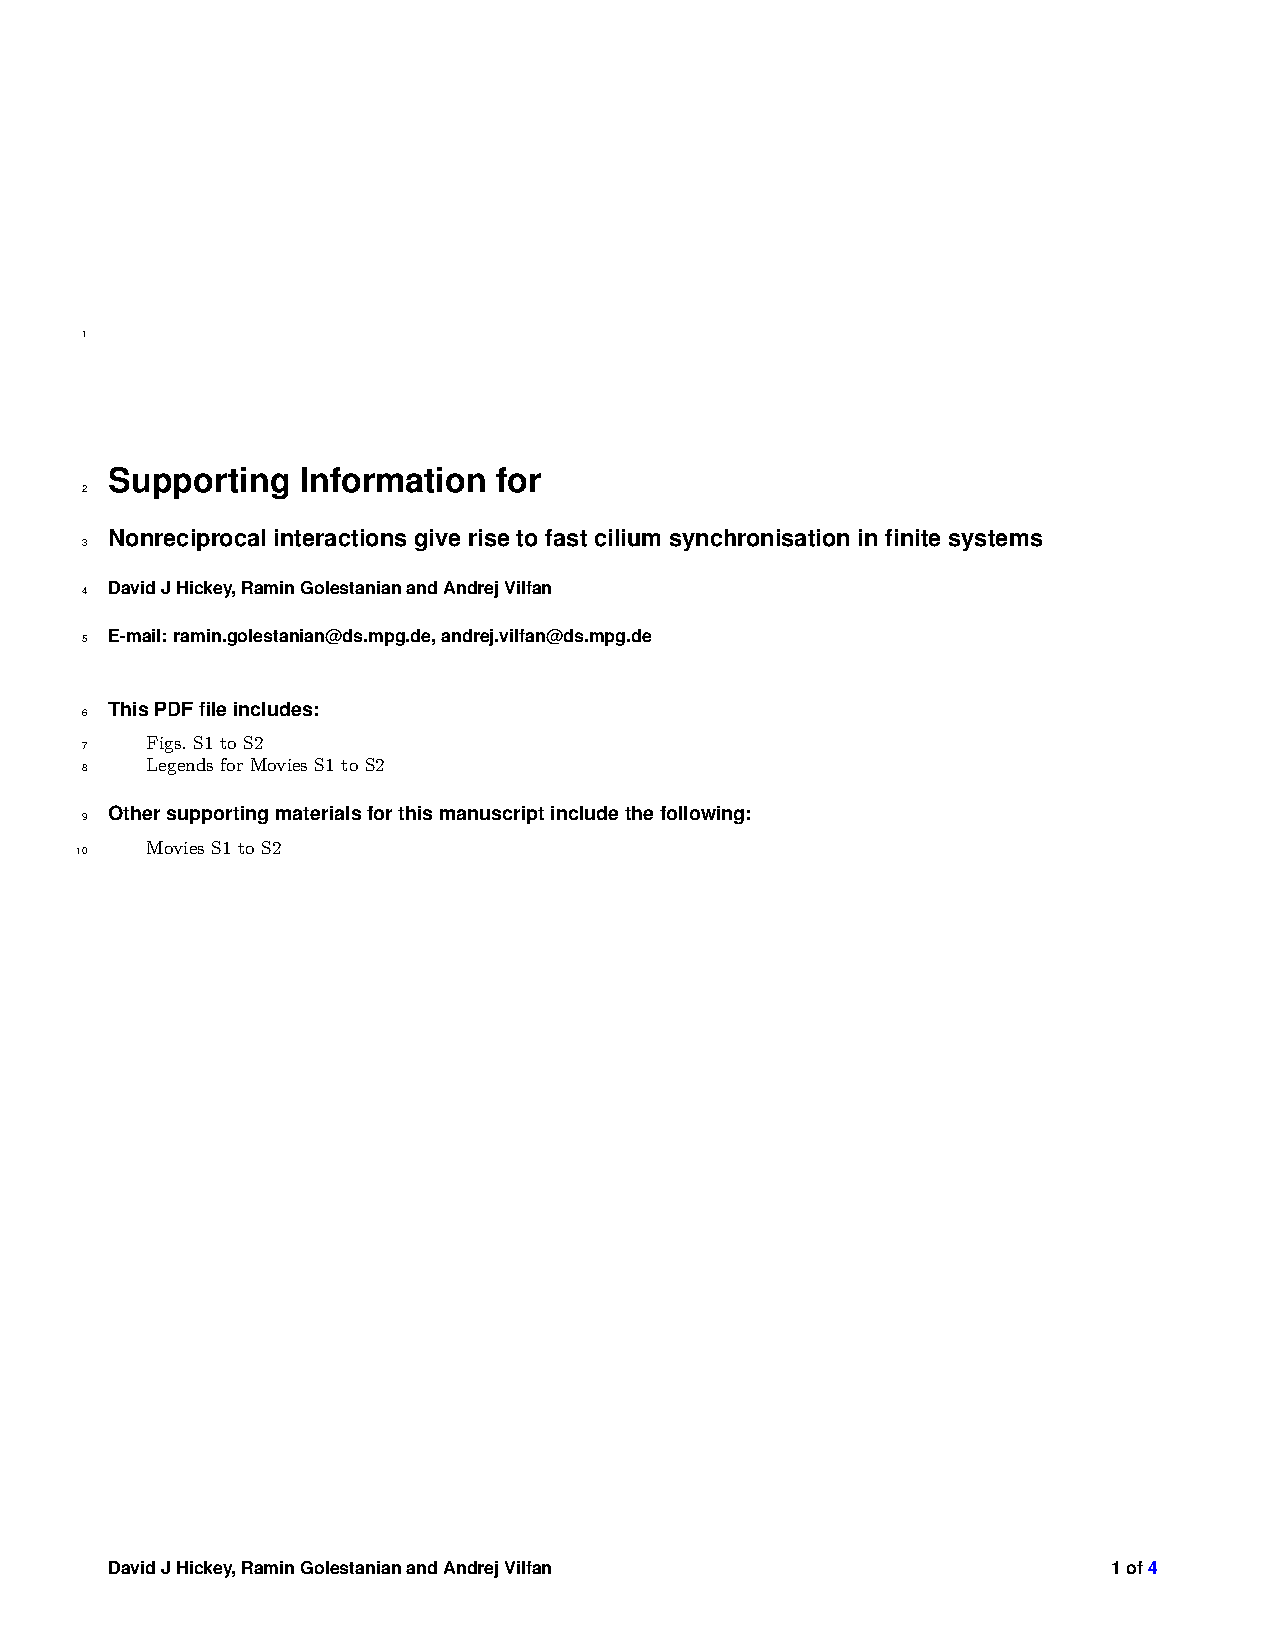
\includepdf[pages=-]{pdfs/Supplement___Nonreciprocal_Interactions____without_branding.pdf}

% As with the previous appendix
% \addtocontents{toc}{\protect\setcounter{tocdepth}{-1}}
% \chapter[Appendix C]{\phantom{X}}
% \addtocontents{toc}{\protect\setcounter{tocdepth}{\sectiontocdepth}}
% \addcontentsline{toc}{chapter}{Appendix C}
% \labch{appendixC}

% \hspace{0pt}
% \vfill
% \begin{fullwidth}
%     \section{List of figures}
% \end{fullwidth}
% \vfill
% \hspace{0pt}

% \listoffigures

%----------------------------------------------------------------------------------------

\backmatter % Denotes the end of the main document content
\setchapterstyle{plain} % Output plain chapters from this point onwards

%----------------------------------------------------------------------------------------
%	BIBLIOGRAPHY
%----------------------------------------------------------------------------------------

% The bibliography needs to be compiled with biber using your LaTeX editor, or on the command line with 'biber main' from the template directory

\printbibliography[heading=bibintoc, title=Bibliography] % Add the bibliography heading to the ToC, set the title of the bibliography and output the bibliography note

% The index needs to be compiled on the command line with 'makeindex main' from the template directory

\printindex % Output the index

%----------------------------------------------------------------------------------------
%	BACK COVER
%----------------------------------------------------------------------------------------

% If you have a PDF/image file that you want to use as a back cover, uncomment the following lines

%\clearpage
%\thispagestyle{empty}
%\null%
%\clearpage
%\includepdf{cover-back.pdf}

%----------------------------------------------------------------------------------------

\clearpage
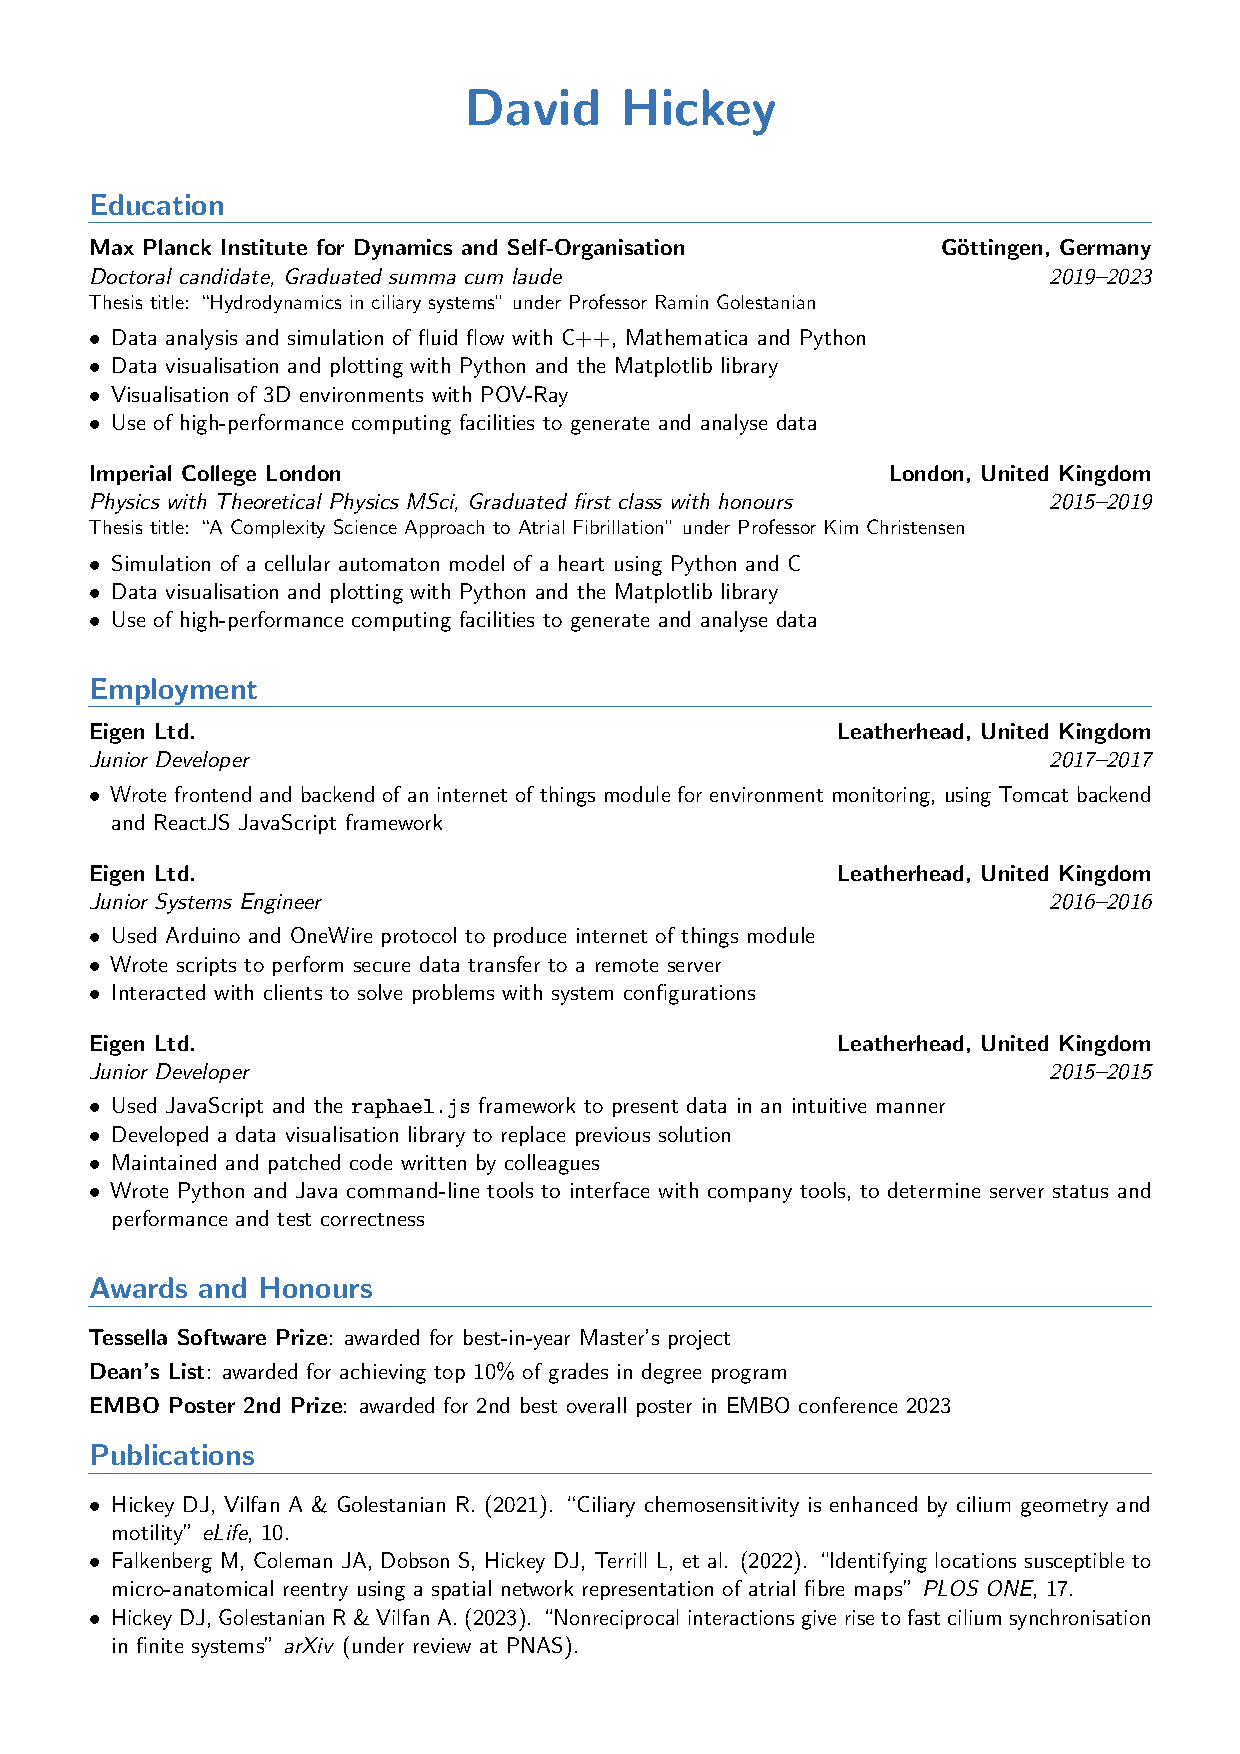
\includepdf[pages=-]{pdfs/Academic_CV.pdf}

\end{document}
